% =====================================================================
%  CD2 drone - complete documentation (single PDF)
%  Build:  pdflatex CD2_Drone_Documentation.tex   (run it twice for the contents)
%  Figures come from the toy model in ../../toy_model3, the Python snippets
%  are read directly from ../../drones_controller.
% =====================================================================
\documentclass[11pt,a4paper]{article}

\usepackage[a4paper, margin=2.3cm, headheight=14pt]{geometry}
\usepackage[T1]{fontenc}
\usepackage{lmodern}
\usepackage{microtype}
\usepackage{amsmath,amssymb,bm,mathtools}
\usepackage{graphicx}
\usepackage{booktabs,array,tabularx}
\usepackage{xcolor}
\usepackage[most]{tcolorbox}
\usepackage{enumitem}
\usepackage{fancyhdr}
\usepackage{titlesec}
\usepackage{caption}
\usepackage{listings}
\usepackage{float}
\usepackage{pdflscape}
\usepackage{needspace}
\usepackage{tikz}
\usetikzlibrary{arrows.meta, positioning}
\usepackage[hidelinks]{hyperref}
\usepackage[nameinlink]{cleveref}

\graphicspath{{figures/}}

% ---------------------------------------------------------------- colours
\definecolor{cHead}{HTML}{B5451B}     % orange-brown, like the MATLAB live script titles
\definecolor{cText}{HTML}{263238}
\definecolor{cToy}{HTML}{A0620F}
\definecolor{cIdea}{HTML}{1565C0}
\definecolor{cReal}{HTML}{2E7D32}
\definecolor{cWarn}{HTML}{B23A48}
\definecolor{cCodeBg}{HTML}{F4F4F4}
\definecolor{cKey}{HTML}{0000FF}
\definecolor{cCom}{HTML}{228B22}
\definecolor{cStr}{HTML}{A020F0}

\hypersetup{colorlinks=true, linkcolor=cHead, urlcolor=cIdea}

\titleformat{\section}{\LARGE\sffamily\color{cHead}}{\thesection}{0.7em}{}
\titleformat{\subsection}{\Large\sffamily\bfseries\color{cText}}{\thesubsection}{0.6em}{}
\titleformat{\subsubsection}{\large\sffamily\bfseries\color{cText}}{\thesubsubsection}{0.5em}{}
\titlespacing*{\section}{0pt}{3ex plus 1ex}{1.5ex}
\titlespacing*{\subsection}{0pt}{2.5ex plus 1ex}{1.0ex}

\pagestyle{fancy}
\fancyhf{}
\fancyhead[L]{\small\sffamily\color{cText!70}CD2 drone \,|\, complete documentation}
\fancyhead[R]{\small\sffamily\color{cText!70}\nouppercase{\leftmark}}
\fancyfoot[C]{\small\sffamily\thepage}
\renewcommand{\headrulewidth}{0.4pt}

\setlength{\parindent}{0pt}
\setlength{\parskip}{6pt}
\setlist{itemsep=2pt, topsep=3pt}
\captionsetup{font=small, labelfont={bf,sf}}
\renewcommand{\arraystretch}{1.15}

% ---------------------------------------------------------------- maths shortcuts
\newcommand{\vp}{\bm{p}}  \newcommand{\vv}{\bm{v}}  \newcommand{\vw}{\bm{\omega}}
\newcommand{\vx}{\bm{x}}  \newcommand{\vu}{\bm{u}}  \newcommand{\vz}{\bm{z}}
\newcommand{\vg}{\bm{g}}  \newcommand{\va}{\bm{a}}  \newcommand{\vF}{\bm{F}}
\newcommand{\vb}{\bm{b}}  \newcommand{\ve}{\bm{e}}  \newcommand{\vtau}{\bm{\tau}}
\newcommand{\vf}{\bm{f}}  \newcommand{\vth}{\bm{\theta}} \newcommand{\vr}{\bm{r}}
\newcommand{\hp}{\hat{\bm p}} \newcommand{\hv}{\hat{\bm v}} \newcommand{\hw}{\hat{\bm\omega}}
\newcommand{\hR}{\hat{R}}     \newcommand{\hx}{\hat{\bm x}}  \newcommand{\vOmega}{\bm{\Omega}}
\newcommand{\skw}[1]{[#1]_{\times}}
\newcommand{\R}{\mathbb{R}}
\newcommand{\SO}{\mathrm{SO}(3)}
\newcommand{\Exp}{\mathrm{Exp}}
\newcommand{\Log}{\mathrm{Log}}
\newcommand{\tr}{\operatorname{tr}}
\newcommand{\diag}{\operatorname{diag}}
\newcommand{\code}[1]{\texttt{\small #1}}

% ---------------------------------------------------------------- boxes
\tcbset{base/.style={enhanced, breakable, boxrule=0.6pt, arc=2pt, left=7pt, right=7pt,
  top=5pt, bottom=5pt, fonttitle=\sffamily\bfseries\small, before skip=8pt, after skip=8pt,
  before upper={\setlength{\parskip}{5pt}}}}
\newtcolorbox{eqbox}[1]{base, colback=cHead!3, colframe=cHead!80, colbacktitle=cHead!80,
  coltitle=white, title={#1}}
\newtcolorbox{toy}[1][]{base, colback=cToy!5, colframe=cToy!70, colbacktitle=cToy!14,
  coltitle=cToy!80!black, title={Toy example\ifx&#1&\else\ --- #1\fi}}
\newtcolorbox{idea}[1][]{base, colback=cIdea!4, colframe=cIdea!60, colbacktitle=cIdea!12,
  coltitle=cIdea!80!black, title={\ifx&#1&The idea in plain words\else #1\fi}}
\newtcolorbox{real}[1][]{base, colback=cReal!5, colframe=cReal!70, colbacktitle=cReal!14,
  coltitle=cReal!70!black, title={How this controls the real drone\ifx&#1&\else\ --- #1\fi}}
\newtcolorbox{warn}[1][]{base, colback=cWarn!5, colframe=cWarn!80, colbacktitle=cWarn!15,
  coltitle=cWarn!80!black, title={\ifx&#1&Be careful\else #1\fi}}

% ---------------------------------------------------------------- code listings
\lstdefinestyle{common}{basicstyle=\ttfamily\small, backgroundcolor=\color{cCodeBg},
  frame=single, rulecolor=\color{black!20}, framesep=4pt, xleftmargin=6pt, xrightmargin=2pt,
  keywordstyle=\color{cKey}, commentstyle=\color{cCom}, stringstyle=\color{cStr},
  showstringspaces=false, breaklines=true, columns=fullflexible, keepspaces=true,
  numberstyle=\tiny\color{black!50}, aboveskip=6pt, belowskip=6pt, upquote=true}
\lstdefinestyle{mat}{style=common, language=Matlab, morekeywords={DroneLib}}
\lstdefinestyle{py}{style=common, language=Python, numbers=left, numbersep=6pt, emptylines=0}
% \pyfile{first line}{last line}{file}{caption}
\newcommand{\pyfile}[4]{\lstinputlisting[style=py, firstline=#1, lastline=#2, firstnumber=#1,
  title={\small\sffamily #4}]{#3}}
\newcommand{\so}{../../drones_controller/drones_controller/so3_controller.py}
\newcommand{\node}{../../drones_controller/drones_controller/controller_node.py}
\newcommand{\sad}{../../drones_controller/drones_controller/state_adapter.py}
\newcommand{\yaml}{../../drones_controller/config/controller.yaml}
\newcommand{\traj}{../../drones_controller/drones_controller/trajectory_generator.py}
% \toycode{file}{section} ... MATLAB code from the toy model
\lstnewenvironment{toycode}[2]{\lstset{style=mat, title={\small\sffamily Toy model: \texttt{toy\_model3/#1.mlx}, section ``#2''}}}{}

% =====================================================================
\begin{document}

\begin{titlepage}
  \centering
  \vspace*{1.2cm}
  {\Huge\sffamily\color{cHead} How Our Drone Knows Where It Is\\[4pt] and How It Is Controlled\\[14pt]}
  {\Large\sffamily\color{cText} The complete mathematics of the CD2 drone,\\ explained step by step with toy examples\\[24pt]}
  {\large\sffamily 3D Mapping of an Environment using a Normal Monocular Camera\\
   and Controlling the Drone by Visual-Inertial Odometry (VIO)\\[6pt]
   Introduction to Drones -- 22AIE448\\[26pt]}
  {\large\sffamily\bfseries Group CD2}\\[6pt]
  {\sffamily Ravishanmugam K \;\textbullet\; Ishwarya Murugesan \;\textbullet\; Aparna Bharani \;\textbullet\; Cibikumar B \;\textbullet\; Akhilan S}\\[4pt]
  {\sffamily School of Artificial Intelligence, Amrita Vishwa Vidyapeetham}
  \vfill
  \begin{minipage}{0.88\linewidth}\small\color{cText}
  \textbf{What this document is.} One place that explains everything in our project: the maths
  of how a drone moves, how it estimates where it is from a camera and an IMU, how it is controlled, and how
  each equation appears in our MATLAB toy model (\code{toy\_model3}) and in our ROS~2 controller
  (\code{drones\_controller}). Nothing is assumed except school algebra and a little calculus. Every new idea
  gets a small example with numbers that you can check with a calculator.
  \end{minipage}
\end{titlepage}

\tableofcontents
\newpage

% =====================================================================
\section{Read This First: the Big Picture}
\label{sec:bigpicture}
% =====================================================================

\subsection{What our project does, in one paragraph}

Our drone carries an ordinary camera (one lens, a \emph{monocular} camera) and an IMU (an Inertial Measurement
Unit: a gyroscope that measures how fast the drone is turning, and an accelerometer). From the camera images we
work out how the drone has moved; this is called \emph{visual odometry}. Mixing that with the IMU is called
\emph{Visual-Inertial Odometry} (VIO). VIO tells the drone where it is, and the same camera poses are used to build
a 3D map of the room. A controller then uses ``where am I'' to decide how to move to ``where I should be''.
In our setup the drone is the Iris quadrotor flying in the Gazebo simulator, ArduPilot (running as SITL,
\emph{Software In The Loop}) is the flight computer, and our own ROS~2 node \code{drones\_controller} is the
controller.

\subsection{The four questions a drone must answer, 25 times every second}

\begin{center}\small
\begin{tabularx}{\linewidth}{@{}>{\raggedright\arraybackslash}p{4.4cm} X >{\raggedright\arraybackslash}p{3.0cm}@{}}
\toprule
\textbf{Question} & \textbf{What answers it in this document} & \textbf{Where}\\
\midrule
1.\ \emph{How does a drone move at all?} & Physics: Newton's law for moving and Euler's law for turning & \Cref{sec:m1b1}--\ref{sec:m1b3}\\
2.\ \emph{Where am I right now?} & The error-state Kalman filter that mixes camera and IMU: our VIO & \Cref{sec:m1b4}\\
3.\ \emph{Where should I go, and how hard should I push?} & A controller: geometric SO(3) control (Model 1) or optimal LQR / MPC (Model 2) & \Cref{sec:m1b5}--\ref{sec:m1b7}, \ref{sec:model2}\\
4.\ \emph{How do I make four motors do that?} & Control allocation: splitting thrust and turning force between the four rotors & \Cref{sec:m1b8}\\
\bottomrule
\end{tabularx}
\end{center}

\subsection{The whole loop in one picture}

\begin{figure}[H]
\centering
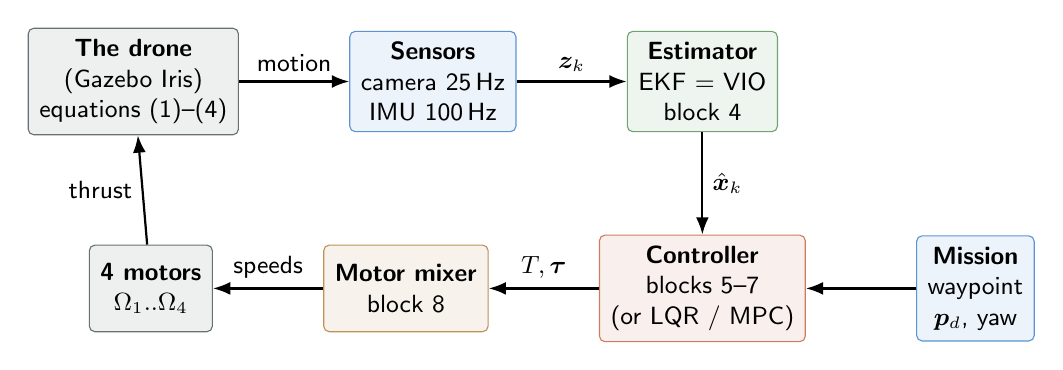
\begin{tikzpicture}[node distance=6mm and 14mm, every node/.style={font=\sffamily\small},
  box/.style={draw, rounded corners=2pt, align=center, minimum height=11mm, inner sep=4pt, fill=#1!8, draw=#1!70},
  arr/.style={-{Latex[length=2.2mm]}, thick}]
  \node[box=cText] (drone) {\textbf{The drone}\\(Gazebo Iris)\\equations (1)--(4)};
  \node[box=cIdea, right=of drone] (sens) {\textbf{Sensors}\\camera 25\,Hz\\IMU 100\,Hz};
  \node[box=cReal, right=of sens] (ekf) {\textbf{Estimator}\\EKF = VIO\\block 4};
  \node[box=cHead, below=13mm of ekf] (ctrl) {\textbf{Controller}\\blocks 5--7\\(or LQR / MPC)};
  \node[box=cToy, left=of ctrl] (mix) {\textbf{Motor mixer}\\block 8};
  \node[box=cText, left=of mix] (mot) {\textbf{4 motors}\\$\Omega_1..\Omega_4$};
  \node[box=cIdea, right=of ctrl] (ref) {\textbf{Mission}\\waypoint\\$\vp_d$, yaw};
  \draw[arr] (drone) -- node[above]{motion} (sens);
  \draw[arr] (sens) -- node[above]{$\vz_k$} (ekf);
  \draw[arr] (ekf) -- node[right]{$\hx_k$} (ctrl);
  \draw[arr] (ref) -- (ctrl);
  \draw[arr] (ctrl) -- node[above]{$T,\vtau$} (mix);
  \draw[arr] (mix) -- node[above]{speeds} (mot);
  \draw[arr] (mot) -- node[left]{thrust} (drone);
\end{tikzpicture}
\caption{The closed loop. The drone moves, the sensors measure it, the estimator works out the state $\hx$,
the controller compares it with the mission and decides thrust $T$ and torque $\vtau$, the mixer turns that into
four motor speeds, and the drone moves again. This repeats every 40\,ms (25\,Hz).}
\label{fig:loop}
\end{figure}

\subsection{Two ways of building the controller: Model 1 and Model 2}

We studied the problem in two ways. Both end with the same four motor speeds.

\begin{itemize}
  \item \textbf{Model 1, the physics way} (\cref{sec:model1}). Write down Newton's and Euler's laws for the drone,
        use them to estimate the state (the EKF) and control the drone with a controller that works directly with
        rotation matrices. This is the structure of our ROS~2 node.
  \item \textbf{Model 2, the data way} (\cref{sec:model2}). Fly, record, let the computer find a simple linear model
        that explains the recording (DMDc), and then compute the best possible controller for that model (LQR), or
        the best plan that also respects limits such as ``never faster than 1\,m/s'' (MPC).
\end{itemize}

The two flow diagrams (\cref{fig:flow1,fig:flow2}) show every block with its equations. Every block number in
those diagrams is a subsection number in this document.



\subsection{How every block is explained}

Every block follows the same pattern, with the same coloured boxes:

\begin{center}\small
\begin{tabularx}{\linewidth}{@{}l X@{}}
\toprule
\textbf{Part} & \textbf{What it gives you}\\
\midrule
\textcolor{cIdea}{\textbf{The idea in plain words}} (blue) & What the block does, with no maths\\
\textcolor{cHead}{\textbf{Equation box}} (orange) & The equations, numbered as in the flow diagram\\
Derivation & Where each equation comes from, one small step at a time\\
\textcolor{cToy}{\textbf{Toy example}} (brown) & Small numbers that you can check with a calculator\\
Toy model code (grey) & The lines of the MATLAB live script in \code{toy\_model3} that compute the equation\\
\textcolor{cReal}{\textbf{How this controls the real drone}} (green) & The lines of our Python controller (with line numbers) and what they do on the drone\\
\bottomrule
\end{tabularx}
\end{center}

\textbf{The toy model.} \code{toy\_model3} contains six MATLAB live scripts (\code{.mlx}) and one helper file
\code{DroneLib.m}. Each live script mixes explanation, equations and code, like the course notes. The
numbers printed in this document are the numbers those scripts print. \Cref{sec:toyguide} explains how to run them.

\begin{landscape}
\begin{figure}[p]
  \centering
  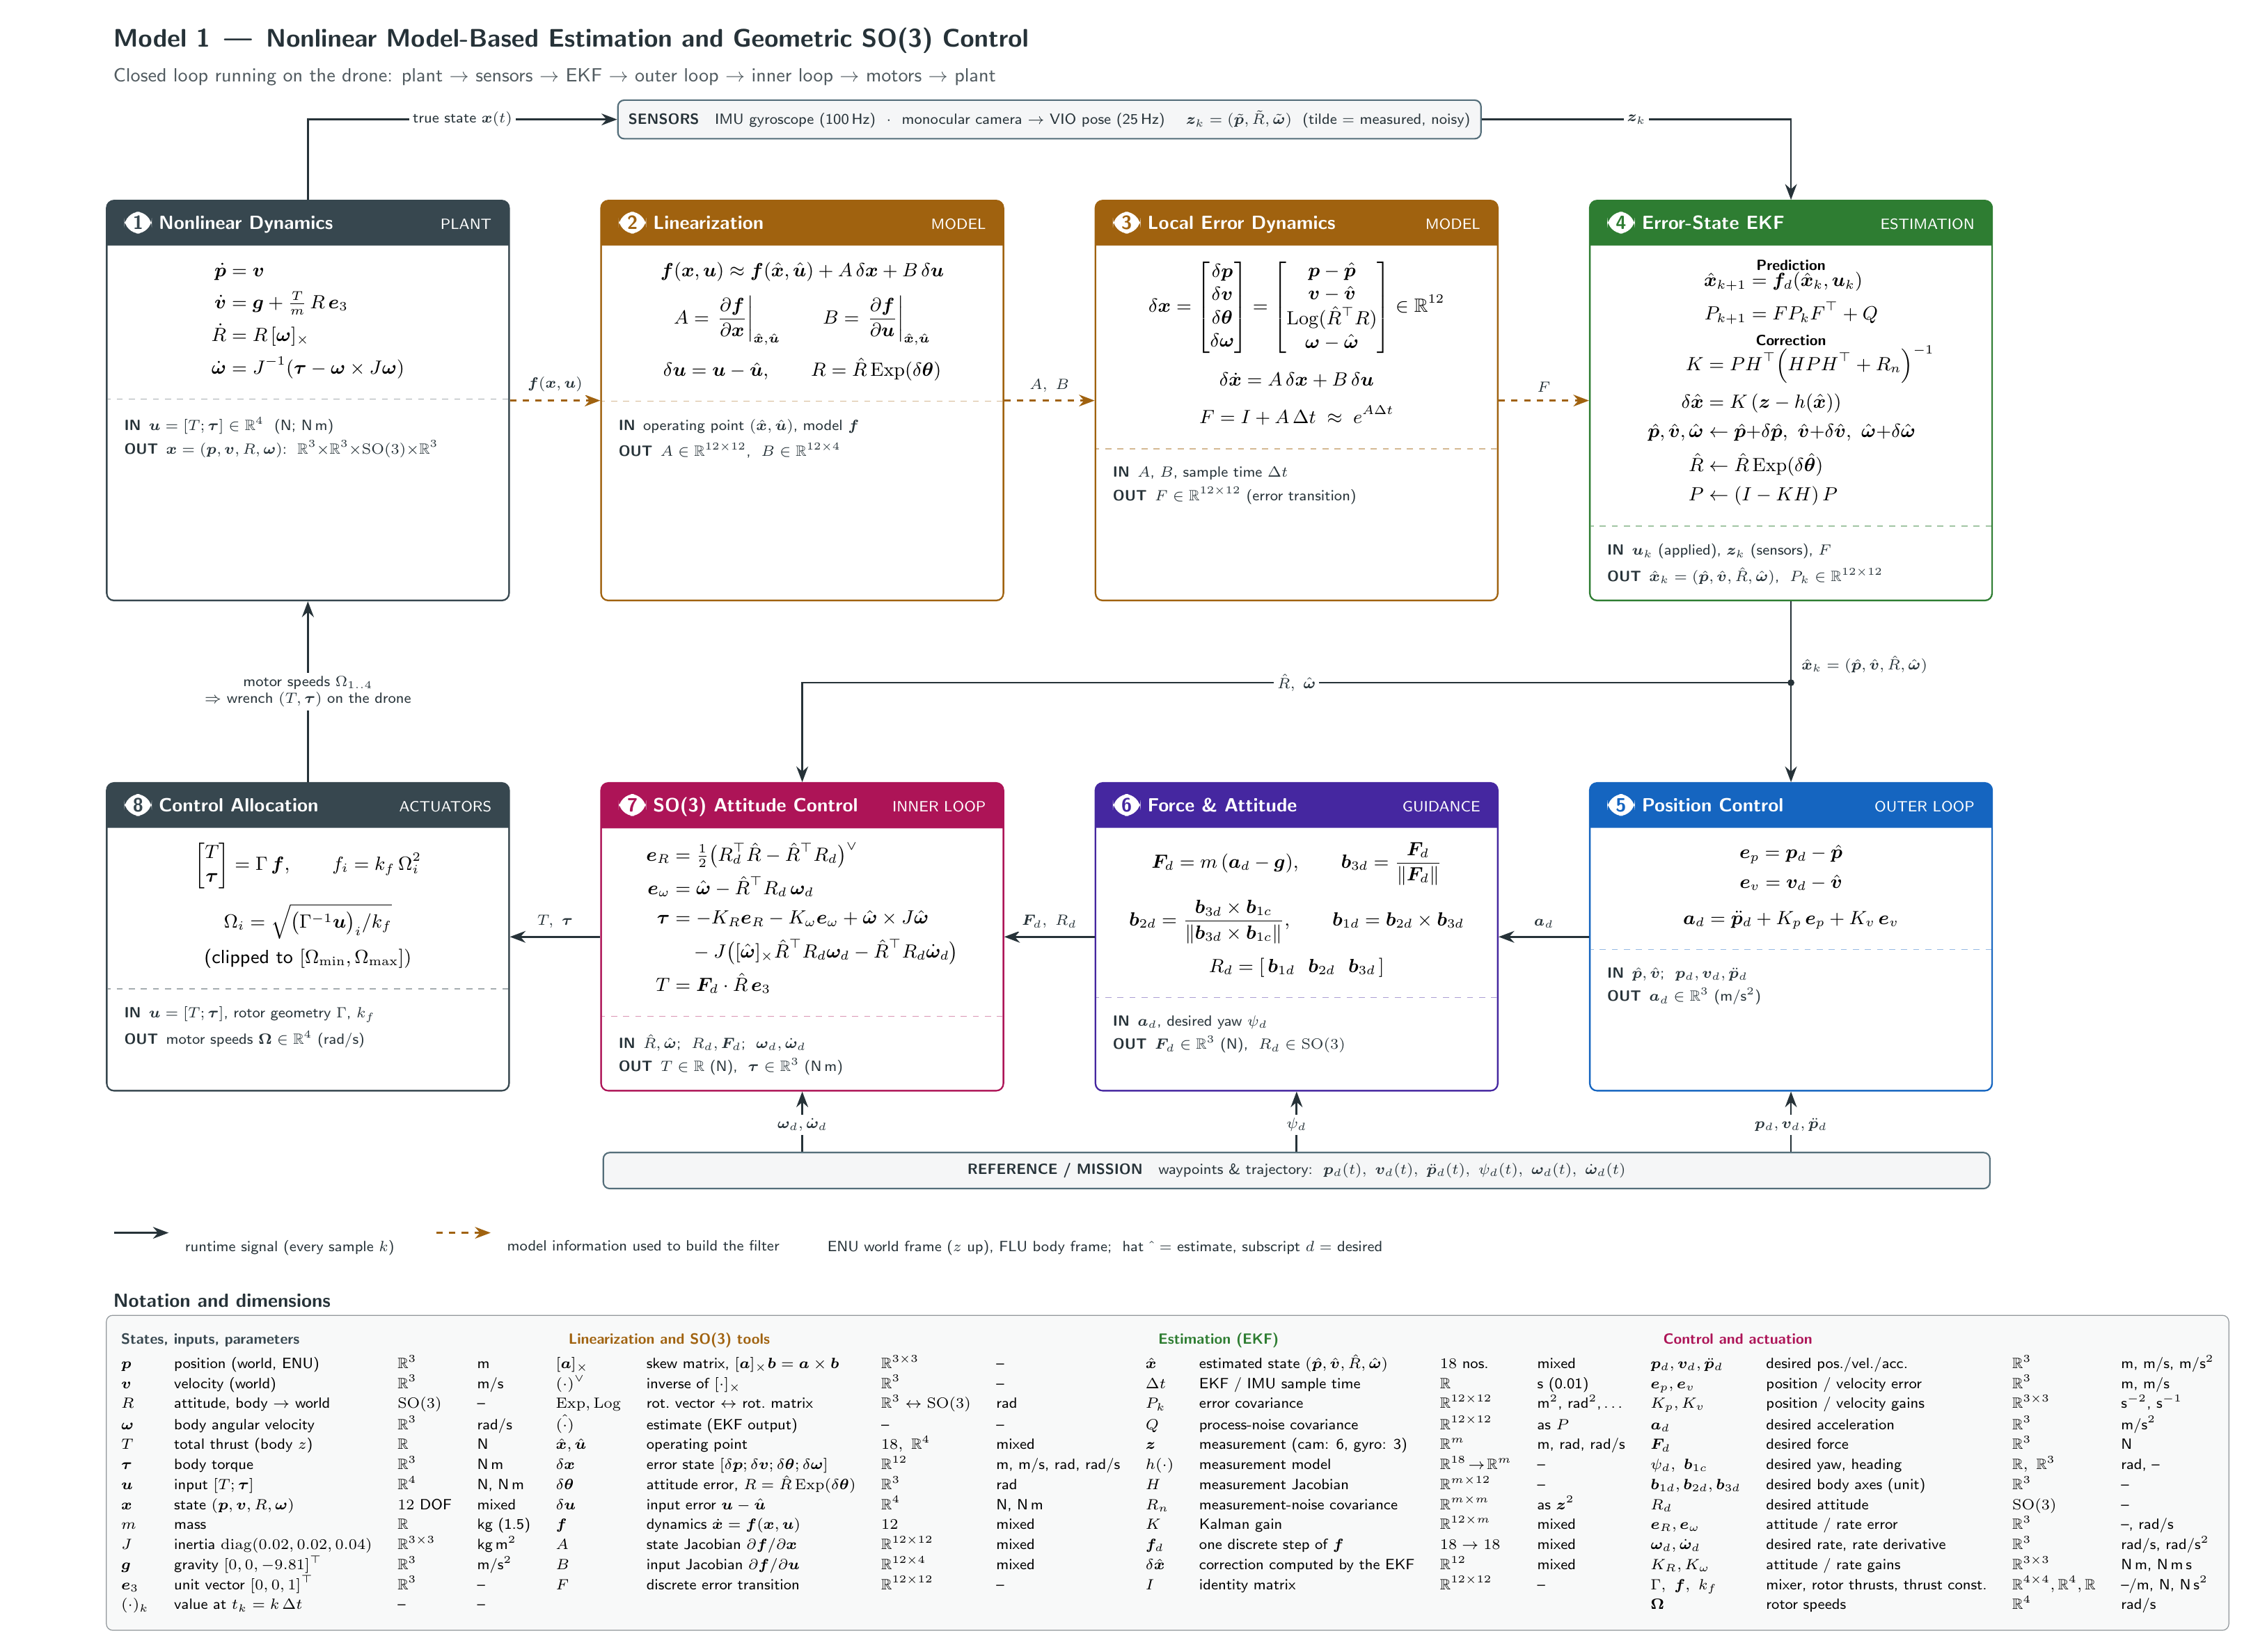
\includegraphics[width=\linewidth,height=0.92\textheight,keepaspectratio]{flow_model1.png}
  \caption{Model 1: nonlinear physics, error-state EKF (our VIO) and geometric SO(3) control.}
  \label{fig:flow1}
\end{figure}
\end{landscape}

\begin{figure}[p]
  \centering
  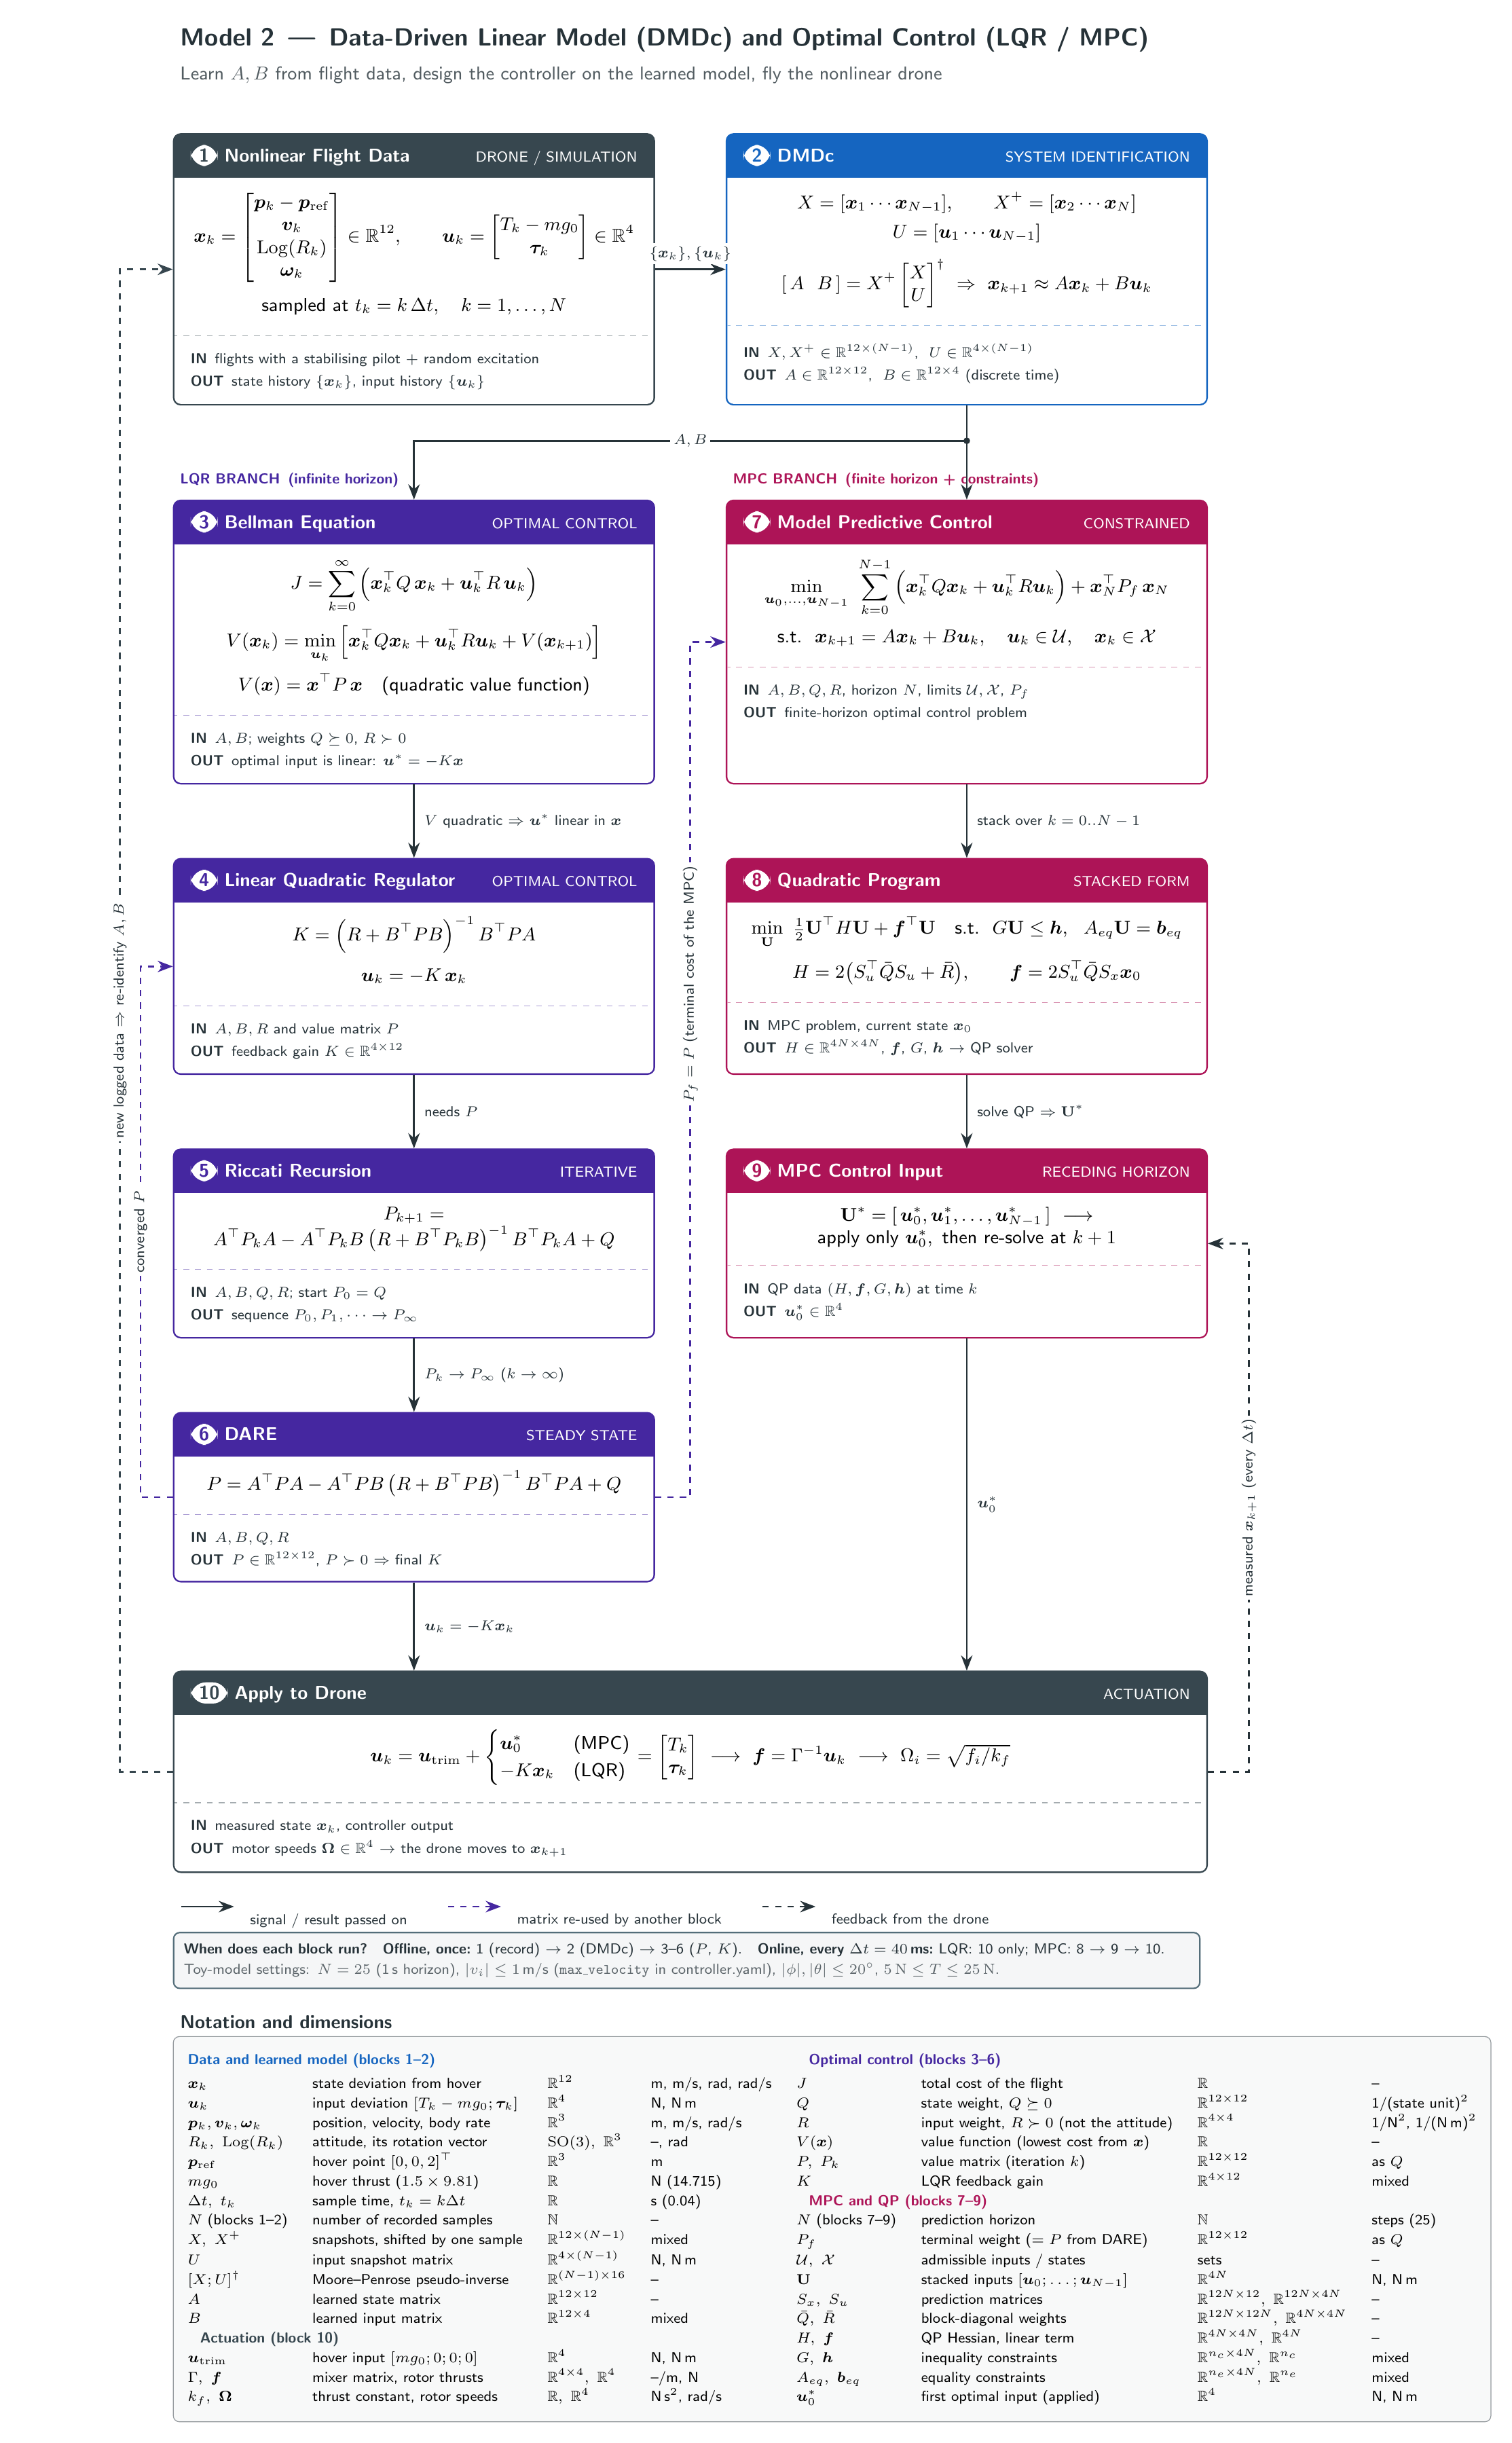
\includegraphics[width=0.86\linewidth]{flow_model2.png}
  \caption{Model 2: a linear model learned from flight data (DMDc), then optimal control by LQR (left branch) or MPC (right branch).}
  \label{fig:flow2}
\end{figure}
\clearpage

% =====================================================================
\section{The Maths Toolbox (everything we need, with tiny examples)}
\label{sec:maths}
% =====================================================================

This section collects every mathematical tool used later. If a later page uses a word you do not know, it is
explained here. Each tool comes with the smallest example that shows how it works.

% ---------------------------------------------------------------------
\subsection{Vectors and matrices}

A \textbf{vector} is a list of numbers written as a column. The position of the drone is a vector with three numbers:
\[
\vp=\begin{bmatrix}p_x\\p_y\\p_z\end{bmatrix}=\begin{bmatrix}0.1\\-0.2\\1.5\end{bmatrix}\ \text{m}
\quad\text{means: 10\,cm east, 20\,cm south, 1.5\,m up.}
\]
We write $\vp\in\R^3$ (``$\vp$ is a list of 3 real numbers''). A \textbf{matrix} is a table of numbers. $M\in\R^{m\times n}$ has
$m$ rows and $n$ columns. Multiplying a matrix by a vector takes each row, multiplies it entry by entry with the vector
and adds up:
\begin{toy}[matrix times vector]
\[
\begin{bmatrix}1&2\\3&4\end{bmatrix}\begin{bmatrix}5\\6\end{bmatrix}=\begin{bmatrix}1\cdot5+2\cdot6\\3\cdot5+4\cdot6\end{bmatrix}=\begin{bmatrix}17\\39\end{bmatrix}.
\]
Sizes must fit: a $4\times12$ matrix times a 12-vector gives a 4-vector. This is exactly what the LQR controller does:
12 errors in, 4 commands out.
\end{toy}

The \textbf{transpose} $M^\top$ swaps rows and columns. For vectors, $\bm a^\top\bm b=a_1b_1+a_2b_2+a_3b_3$ is the
\textbf{dot product}; it measures how much two vectors point the same way. $\|\bm a\|=\sqrt{\bm a^\top\bm a}$ is the length.
The \textbf{cross product} $\bm a\times\bm b$ is a vector at right angles to both:
\begin{toy}[dot and cross product]
$\bm a=[1,0,0]$ (east), $\bm b=[0,1,0]$ (north): $\bm a^\top\bm b=0$ (they are at right angles),
$\bm a\times\bm b=[0,0,1]$ (up). Rule: $\bm a\times\bm b=[a_2b_3-a_3b_2,\ a_3b_1-a_1b_3,\ a_1b_2-a_2b_1]$.
\end{toy}

The \textbf{identity matrix} $I$ has ones on the diagonal and zeros elsewhere; $I\bm a=\bm a$. The \textbf{inverse}
$M^{-1}$ undoes $M$: $M^{-1}M=I$. $\diag(a,b,c)$ is a matrix with $a,b,c$ on the diagonal and zeros elsewhere.

% ---------------------------------------------------------------------
\subsection{Rates of change and differential equations}

A dot on top means ``rate of change with time'': $\dot{\vp}=d\vp/dt$ is velocity and $\ddot{\vp}$ is acceleration.
An equation of the form
\[
\dot{\vx}=\vf(\vx,\vu)
\]
is a \textbf{differential equation}. It does not tell you where the system is; it tells you \emph{how fast it is
changing}, given where it is ($\vx$, the \textbf{state}) and what you are doing to it ($\vu$, the \textbf{input}).
A computer finds the motion by taking small time steps $\Delta t$.
\begin{toy}[Euler's method for a falling ball]
State $x=[\text{height};\ \text{velocity}]$, $\dot x=[\text{velocity};\ -9.81]$. Start at height 10\,m, at rest,
$\Delta t=0.1$\,s. One step: $\text{height}=10+0.1\cdot0=10$, $\text{velocity}=0+0.1\cdot(-9.81)=-0.981$.
Next step: $\text{height}=10+0.1\cdot(-0.981)=9.902$\,m, and so on. Each step is ``new = old + $\Delta t\,\times$ rate''.
The course notes do exactly this for the Lotka--Volterra and Lorenz systems.
\end{toy}

Euler's method is simple but not very accurate. The toy model uses \textbf{RK4} (Runge--Kutta of order 4), which
looks at the rate four times inside the step (start, two in the middle, end) and averages them. MATLAB's \code{ode45}
uses the same idea with automatic step sizes.

\textbf{Discrete time.} A computer works in ticks $t_k=k\,\Delta t$. A subscript $k$ means ``at tick $k$''. So
$\vx_{k+1}=A\vx_k+B\vu_k$ reads: next state $=$ (matrix) $\times$ current state $+$ (matrix) $\times$ current input.
Model 2 works entirely in this form.

% ---------------------------------------------------------------------
\subsection{Taylor series and linearization}
\label{sec:taylor}

From the course notes: if we know a smooth function $f$ and its derivatives at a point $a$, we can predict it nearby:
\[
f(x)=f(a)+f'(a)(x-a)+\frac{f''(a)}{2!}(x-a)^2+\dots
\]
Keeping only the first two terms gives the \textbf{first order (linear) approximation}: near $a$ the curve looks like
its tangent line.
\begin{toy}[$\sin$ near 0]
$f(\theta)=\sin\theta$, $a=0$: $f(0)=0$, $f'(0)=\cos0=1$, so $\sin\theta\approx\theta$.
For $\theta=0.1$\,rad: true $0.0998$, linear $0.1$ (0.17\% off). For $\theta=0.5$\,rad: true $0.479$, linear $0.5$
(4.3\% off). The approximation is excellent close to $a$ and gets worse further away. This exact example decides how
well the linear drone models work: $\theta$ is the tilt of the drone.
\end{toy}

For a function of \emph{many} variables that also gives \emph{many} outputs, the slopes form a matrix, the
\textbf{Jacobian}. Entry $(i,j)$ is $\partial f_i/\partial x_j$: ``how much output $i$ changes when only input $j$ is
nudged''. Then
\[
\vf(\vx)\approx\vf(\bm a)+J\,(\vx-\bm a),\qquad J=\left.\frac{\partial\vf}{\partial\vx}\right|_{\bm a}.
\]
\begin{toy}[a Jacobian by hand]
$\vf(x,y)=\begin{bmatrix}x\,y\\ x+y^2\end{bmatrix}$ at $(x,y)=(2,1)$:\quad
$J=\begin{bmatrix}\partial f_1/\partial x&\partial f_1/\partial y\\ \partial f_2/\partial x&\partial f_2/\partial y\end{bmatrix}=
\begin{bmatrix}y&x\\1&2y\end{bmatrix}=\begin{bmatrix}1&2\\1&2\end{bmatrix}$.

Move to $(2.1,\,1)$: the linear prediction is $\vf(2,1)+J[0.1,0]^\top=[2,3]+[0.1,0.1]=[2.1,3.1]$. The true value is
$[2.1\cdot1,\ 2.1+1]=[2.1,3.1]$. Here they agree exactly because $\vf$ is linear in $x$.
\end{toy}

\textbf{Linear versus nonlinear.} A model is \emph{linear} if doubling the input doubles the effect, like
$\vx_{k+1}=A\vx_k+B\vu_k$. A drone is \emph{nonlinear} because of $\sin$, $\cos$ and products like $\vw\times J\vw$.
Linear models are much easier to work with, so we \textbf{linearize}: replace the nonlinear model by its Jacobian
near an \textbf{operating point} such as hover.

% ---------------------------------------------------------------------
\subsection{Rotations: the rotation matrix $R$}
\label{sec:rotations}

The \textbf{attitude} (orientation) of the drone is stored as a $3\times3$ \textbf{rotation matrix} $R$. Its three
columns are the drone's own three axes (forward, left, up), written in world coordinates:
\[
R=\big[\ \vb_1\ \ \vb_2\ \ \vb_3\ \big],\qquad \vb_1=\text{drone's nose},\ \vb_2=\text{drone's left},\ \vb_3=\text{drone's top}.
\]
Multiplying $R$ by a vector written in the drone's frame gives the same vector in the world frame.
\begin{toy}[the drone turned 90 degrees to the left (yaw)]
Its nose now points north, its left points west, its top still points up:
$R=\begin{bmatrix}0&-1&0\\1&0&0\\0&0&1\end{bmatrix}$.
A camera that looks along the nose, $[1,0,0]$ in the drone frame, looks along $R[1,0,0]^\top=[0,1,0]^\top$: north. Correct.
\end{toy}

Every rotation matrix has two properties: the columns are unit length and at right angles, which is written
$R^\top R=I$ (so $R^{-1}=R^\top$), and $\det R=+1$ (it is not a mirror). The set of all such matrices is called
$\SO$ (``special orthogonal group in 3D''). When you see $\SO$, read ``rotation matrices''.

\textbf{Why not roll, pitch, yaw angles?} Three angles are easier to imagine, but they break down: at a pitch of
$90^\circ$ the roll and yaw axes line up and one direction of motion is lost (\textbf{gimbal lock}). Rotation matrices
never break down. That is why our controller is called \emph{geometric} or \emph{SO(3)} control: it works with $R$
directly.

% ---------------------------------------------------------------------
\subsection{The hat and vee maps}

A cross product can be written as a matrix times a vector. For $\bm a=[a_1,a_2,a_3]$:
\[
\skw{\bm a}=\begin{bmatrix}0&-a_3&a_2\\a_3&0&-a_1\\-a_2&a_1&0\end{bmatrix},\qquad \skw{\bm a}\,\bm b=\bm a\times\bm b .
\]
$\skw{\cdot}$ is called \textbf{hat}. The matrix is \emph{skew-symmetric}: $\skw{\bm a}^\top=-\skw{\bm a}$. The reverse
operation, which reads the three numbers back out of such a matrix, is called \textbf{vee}: $\skw{\bm a}^\vee=\bm a$.
\begin{toy}[hat and vee]
$\bm a=[1,2,3]$: $\skw{\bm a}=\begin{bmatrix}0&-3&2\\3&0&-1\\-2&1&0\end{bmatrix}$. Then vee takes entries (3,2), (1,3), (2,1):
$[1,\,2,\,3]$. In our Python code these are \code{hat()} and \code{vee()} in \code{state\_adapter.py}.
\end{toy}

% ---------------------------------------------------------------------
\subsection{Exp and Log: rotation vector $\leftrightarrow$ rotation matrix}

A rotation can also be described by a \textbf{rotation vector} $\bm\phi=\theta\,\bm n$: turn by the angle $\theta$
about the unit axis $\bm n$. The two descriptions are linked by
\[
\Exp(\bm\phi)=I+\sin\theta\,\skw{\bm n}+(1-\cos\theta)\skw{\bm n}^2\quad\text{(Rodrigues' formula)},\qquad \Log(R)=\bm\phi .
\]
For a \emph{small} rotation, $\Exp(\bm\phi)\approx I+\skw{\bm\phi}$. This is used everywhere to describe a small
attitude error with 3 numbers instead of 9.
\begin{toy}[90 degrees about the vertical axis]
$\bm n=[0,0,1]$, $\theta=\pi/2$: $\sin\theta=1$, $1-\cos\theta=1$, $\skw{\bm n}^2=\diag(-1,-1,0)$, so
$\Exp=I+\skw{\bm n}+\diag(-1,-1,0)=\begin{bmatrix}0&-1&0\\1&0&0\\0&0&1\end{bmatrix}$, which is the yaw matrix of the earlier example.
And $\Log$ of that matrix gives back $[0,0,1.5708]$.
\end{toy}

% ---------------------------------------------------------------------
\subsection{Uncertainty: mean, variance, covariance}

Sensors are noisy, so we need words for ``how unsure''. The \textbf{mean} is the average. The \textbf{variance}
$\sigma^2$ is the average squared distance from the mean, and the \textbf{standard deviation} $\sigma$ is the typical
size of the error. For a vector of errors, the \textbf{covariance matrix} $P=\mathbb E[\bm e\bm e^\top]$ holds the
variance of each component on its diagonal and ``how two components move together'' off the diagonal.
A \textbf{Gaussian} (bell curve) $\mathcal N(\mu,\sigma^2)$ puts about 68\% of samples within $\pm\sigma$ and 99.7\%
within $\pm3\sigma$.
\begin{toy}[three altitude readings]
Readings $9.8,\ 10.1,\ 10.1$\,m: mean $10.0$, deviations $-0.2,\ 0.1,\ 0.1$,
variance $(0.04+0.01+0.01)/3=0.02$\,m$^2$, $\sigma=0.14$\,m.
\end{toy}

\textbf{The one rule we use again and again.} If an error vector is multiplied by a matrix, $\bm e'=F\bm e$, its
covariance becomes
\[
P'=\mathbb E[F\bm e\bm e^\top F^\top]=F\,P\,F^\top .
\]
\begin{toy}[uncertainty grows when you integrate]
Position and velocity errors $[\delta p,\delta v]$ with $P=\diag(0.01,\ 0.04)$ (10\,cm and 20\,cm/s). After 1\,s,
$\delta p'=\delta p+1\cdot\delta v$, $\delta v'=\delta v$, so $F=\begin{bmatrix}1&1\\0&1\end{bmatrix}$ and
$P'=FPF^\top=\begin{bmatrix}0.05&0.04\\0.04&0.04\end{bmatrix}$. The position variance grew from 0.01 to 0.05
($\sigma$ from 10 to 22\,cm), because an unknown velocity turns into an unknown position.
\end{toy}

% ---------------------------------------------------------------------
\subsection{Finding the lowest point of a bowl}
\label{sec:minquad}

At the bottom of a smooth curve the slope is zero. For $g(u)=au^2+bu+c$ with $a>0$ (a bowl):
\[
g'(u)=2au+b=0\quad\Longrightarrow\quad u^*=-\frac{b}{2a}.
\]
The many-variable version: for $g(\vu)=\vu^\top M\vu+\bm b^\top\vu$ with $M$ ``positive definite'' (a bowl in every
direction, meaning $\vu^\top M\vu>0$ for every $\vu\neq0$), the gradient is $2M\vu+\bm b=\bm0$, so
$\vu^*=-\tfrac12M^{-1}\bm b$. Both the Kalman gain and the LQR gain are found exactly like this.
\begin{toy}[a one-dimensional bowl]
$g(u)=u^2-4u+1$: $g'(u)=2u-4=0\Rightarrow u^*=2$, and $g(2)=-3$ is the lowest value.
\end{toy}

% ---------------------------------------------------------------------
\subsection{Eigenvalues: will it blow up or die out?}
\label{sec:eig}

If $M\bm v=\lambda\bm v$, the direction $\bm v$ is only stretched by $M$, by the factor $\lambda$ (an
\textbf{eigenvalue}). For $\vx_{k+1}=M\vx_k$, every such direction is multiplied by $\lambda$ at every tick, so
\[
\text{all }|\lambda|<1\ \Rightarrow\ \text{the state dies out (stable)};\qquad
\text{some }|\lambda|>1\ \Rightarrow\ \text{it blows up (unstable)}.
\]
The largest $|\lambda|$ is called the \textbf{spectral radius} $\rho(M)$.
\begin{toy}[two scalar systems]
$x_{k+1}=1.1\,x_k$: $1,\ 1.1,\ 1.21,\ 1.33,\dots$ grows for ever.\quad
$x_{k+1}=0.62\,x_k$: $1,\ 0.62,\ 0.38,\ 0.24,\dots$ dies out. \Cref{sec:m2b4} shows that LQR turns the first system into the second.
\end{toy}
For continuous-time systems $\dot\vx=M\vx$ the rule is about the real part instead: all eigenvalues with negative
real part means stable.

% ---------------------------------------------------------------------
\subsection{Least squares and the pseudo-inverse}
\label{sec:lsq}

Given many noisy examples, find the one rule that fits them best. If the rule is $y\approx g\,x$ and we have samples
$(x_i,y_i)$, the \textbf{least-squares} choice minimises $\sum_i(y_i-g\,x_i)^2$. Setting the derivative to zero gives
$g=\sum x_iy_i/\sum x_i^2$. For many rows at once, with all inputs as columns of $\Omega$ and all outputs as
columns of $Y$:
\[
G=Y\,\Omega^\top(\Omega\Omega^\top)^{-1}=Y\,\Omega^\dagger .
\]
$\Omega^\dagger$ is the \textbf{pseudo-inverse} (MATLAB: \code{pinv}). It is the EDMD formula
\code{K = Psi2*pinv(Psi1)} from the course notes, and DMDc in \cref{sec:m2b2}.
\begin{toy}[fitting a slope]
Samples $(1,2.1),\ (2,3.9),\ (3,6.0)$: $\sum xy=2.1+7.8+18=27.9$, $\sum x^2=14$, so $g=1.993$, close to the
true slope 2.
\end{toy}

% =====================================================================
\section{Our Drone and Our Software}
\label{sec:setup}
% =====================================================================

\subsection{The pieces of the system}

\begin{center}\small
\begin{tabularx}{\linewidth}{@{}l X@{}}
\toprule
\textbf{Piece} & \textbf{What it does for us}\\
\midrule
Gazebo + Iris model & The ``real'' drone: a 3D physics simulator that solves the equations of motion of a 1.5\,kg quadrotor\\
ArduPilot SITL & The flight computer software, running on the PC. It reads the simulated IMU, runs its own
  estimator (EKF3) and its own low-level controllers, and drives the four motors\\
ROS~2 & The ``post office'' between programs. Programs publish and subscribe to named \emph{topics}\\
Monocular camera + VIO & Images $\rightarrow$ visual odometry pose; fused with the IMU it gives the state; the same poses build the 3D map\\
\code{drones\_controller} & Our ROS~2 package: reads the state, runs the SO(3) controller, sends commands\\
\code{toy\_model3} & Our MATLAB toy model: every equation of this document, runnable, with small examples\\
\bottomrule
\end{tabularx}
\end{center}

The ROS~2 topics that matter:

\begin{center}\small
\begin{tabularx}{\linewidth}{@{}l l X@{}}
\toprule
\textbf{Topic} & \textbf{Direction} & \textbf{Content}\\
\midrule
\code{/ap/v1/pose/filtered} & ArduPilot $\rightarrow$ us & position $\vp$ and orientation (quaternion $\rightarrow R$), from ArduPilot's EKF\\
\code{/ap/v1/twist/filtered} & ArduPilot $\rightarrow$ us & velocity $\vv$ and angular velocity $\vw$\\
\code{/ap/v1/cmd\_vel} & us $\rightarrow$ ArduPilot & the velocity command we want the drone to fly\\
\code{/drones\_controller/*} & us $\rightarrow$ anyone & our diagnostics: $\ve_p,\ve_v,\vF_d,\vtau,\ve_R,\ve_\omega,R_d$\\
\bottomrule
\end{tabularx}
\end{center}

\subsection{Frames: which way is up?}

\begin{itemize}
  \item \textbf{World frame, ENU}: $x$ = East, $y$ = North, $z$ = Up. ArduPilot's ROS~2 topics use this. Gravity
        is therefore $\vg=[0,\ 0,\ -9.81]^\top$\,m/s$^2$ (it pulls towards $-z$).
  \item \textbf{Body frame, FLU}: fixed to the drone, $x$ = Forward (nose), $y$ = Left, $z$ = Up (through the
        propellers). The thrust always points along body $+z$.
  \item The rotation matrix $R$ turns body-frame vectors into world-frame vectors (\cref{sec:rotations}).
\end{itemize}

\subsection{The state of the drone}

Everything we need to know about the drone at one moment is its \textbf{state}:
\begin{center}\small
\begin{tabular}{@{}l l l l@{}}
\toprule
\textbf{Symbol} & \textbf{Meaning} & \textbf{Size} & \textbf{Unit}\\
\midrule
$\vp$ & position (world) & 3 numbers & m\\
$\vv$ & velocity (world) & 3 numbers & m/s\\
$R$ & attitude: rotation body $\rightarrow$ world & $3\times3$ matrix & --\\
$\vw$ & angular velocity, measured in the body (what a gyro reads) & 3 numbers & rad/s\\
\bottomrule
\end{tabular}
\end{center}
That is 18 stored numbers but only 12 ``degrees of freedom'', because $R$ has 9 entries but only 3 independent
directions of rotation. The \textbf{input} is $\vu=[T;\ \vtau]$: total thrust $T$ (newtons) and the three body
torques $\vtau$ (newton-metres).

A hat on a symbol means \emph{estimated} ($\hp$ = the position the estimator believes). A subscript $d$ means
\emph{desired} ($\vp_d$ = where we want to be). A tilde means \emph{measured by a sensor} ($\tilde{\vp}$).

\subsection{The parameters: \texttt{controller.yaml}}

All numbers used in this document and in the toy model come from the configuration file of our controller:

\lstinputlisting[style=py, language={}, title={\small\sffamily drones\_controller/config/controller.yaml}]{\yaml}

\begin{center}\small
\begin{tabular}{@{}l l l@{}}
\toprule
\textbf{YAML key} & \textbf{Symbol in this document} & \textbf{Value}\\
\midrule
\code{mass}, \code{gravity} & $m$, $g_0$ & 1.5\,kg, 9.81\,m/s$^2$\\
\code{inertia} & $J=\diag(J_x,J_y,J_z)$ & $\diag(0.02,\ 0.02,\ 0.04)$\,kg\,m$^2$\\
\code{kp}, \code{kv} & $K_p$, $K_v$ (position loop) & $\diag(1.5,1.5,2.0)$, $\diag(1.2,1.2,1.5)$\\
\code{kR}, \code{kOmega} & $K_R$, $K_\omega$ (attitude loop) & $\diag(4,4,2)$, $\diag(0.8,0.8,0.5)$\\
\code{desired\_x/y/z}, \code{desired\_yaw} & $\vp_d$, $\psi_d$ & $[0,0,2]$\,m, 0\,rad\\
\code{control\_rate} & $1/\Delta t$ & 25\,Hz ($\Delta t=0.04$\,s)\\
\code{max\_velocity} & speed limit & 1.0\,m/s\\
\code{state\_timeout} & how old the state may be & 0.5\,s\\
\code{enable\_command} & actually send commands? & \code{false} by default (safety)\\
\bottomrule
\end{tabular}
\end{center}

The rotor numbers (arm positions, thrust constant $k_f=8.549\times10^{-6}$\,N\,s$^2$, yaw constant $c_m=0.016$\,m)
are those of the ArduPilot Gazebo Iris. They are only needed in the motor mixer (\cref{sec:m1b8}).

% =====================================================================
\section{Model 1: Physics, Estimation and Geometric Control}
\label{sec:model1}
% =====================================================================

Model~1 is the loop that flies the drone (\cref{fig:flow1}). Blocks 1--3 describe how the drone moves and how a small
error grows. Block 4 estimates the state from the sensors. Blocks 5--7 decide thrust and torque. Block 8 turns them
into motor speeds. Toy model files: \code{M1\_1\_Dynamics\_Linearization.mlx} (blocks 1--3),
\code{M1\_2\_Error\_State\_EKF.mlx} (block 4) and\\ \code{M1\_3\_SO3\_Control\_Closed\_Loop.mlx} (blocks 5--8).

% ---------------------------------------------------------------------
\subsection{Block 1 --- How the drone moves (nonlinear dynamics)}
\label{sec:m1b1}
% ---------------------------------------------------------------------

\begin{idea}
A quadrotor is one solid body. Its four propellers can only push in one direction: straight out of the top of
the drone. Gravity pulls it down. To move sideways it must first \emph{tilt}, so that part of its push points
sideways. To tilt, the rotors push unevenly, which creates a twisting force (torque). So there are two
connected stories: how the body \emph{moves} (Newton) and how it \emph{turns} (Euler).
\end{idea}

\begin{eqbox}{Equations (1)--(4): rigid-body dynamics of the quadrotor}
\begin{align}
  \dot{\vp} &= \vv \tag{1}\label{eq:1}\\
  \dot{\vv} &= \vg + \frac{T}{m}\,R\,\ve_3 \tag{2}\label{eq:2}\\
  \dot{R}   &= R\,\skw{\vw} \tag{3}\label{eq:3}\\
  \dot{\vw} &= J^{-1}\big(\vtau - \vw\times J\vw\big) \tag{4}\label{eq:4}
\end{align}
State $\vx=(\vp,\vv,R,\vw)$, input $\vu=[T;\ \vtau]$, $\ve_3=[0,0,1]^\top$. In short: $\dot\vx=\vf(\vx,\vu)$.
\end{eqbox}

\subsubsection*{Where each equation comes from}

\textbf{(1) Position.} Velocity is, by definition, how fast position changes: $\vv=d\vp/dt$. Nothing more.

\textbf{(2) Newton's second law, $m\,\dot{\vv}=$ sum of forces.} Two forces act on the drone.
\begin{enumerate}
  \item Gravity: $m\vg=m[0,0,-9.81]^\top$, always straight down.
  \item Thrust: the four rotors together push with $T$ newtons along the drone's own up-axis. In the body frame this
        is $T\ve_3=[0,0,T]^\top$. To write it in the world frame we multiply by $R$ (\cref{sec:rotations}):
        $R\,T\ve_3=T\,\vb_3$, where $\vb_3$ is the third column of $R$, the direction the top of the drone points.
\end{enumerate}
So $m\dot\vv=m\vg+T R\ve_3$. Dividing by $m$ gives (2). Air drag and wind are left out of the model. In the toy
simulation they are added as unknown ``gusts'', which is exactly what the controller has to cope with.

\textbf{(3) How the attitude changes.} Take a point fixed on the drone, at $\bm r$ in body coordinates. In the world
it is at $R\bm r$, so its velocity is $\dot R\,\bm r$. A body spinning with angular velocity $\vw$ (measured in the body)
moves that point with velocity $\vw\times\bm r$ in body coordinates, which is $R(\vw\times\bm r)=R\skw{\vw}\bm r$ in
the world. Since this holds for every $\bm r$: $\dot R=R\skw{\vw}$. This is how the gyroscope reading $\vw$ turns the
attitude.

\textbf{(4) Euler's law for rotation.} The ``spin momentum'' (angular momentum) is $J\vw$, where $J$ is the
inertia matrix (how hard the body is to spin about each axis). Torque changes angular momentum. Because the body
frame itself is turning, an extra term appears:
\[
J\dot{\vw}+\vw\times J\vw=\vtau\quad\Longrightarrow\quad \dot\vw=J^{-1}(\vtau-\vw\times J\vw).
\]
The term $\vw\times J\vw$ is the \textbf{gyroscopic coupling}: spinning about two axes at once starts a spin about the
third axis, even with no torque. (Derivation: the world-frame momentum is $\bm h=RJ\vw$; Newton for rotation says
$\dot{\bm h}=R\vtau$; differentiating with (3) gives $R(\skw{\vw}J\vw+J\dot\vw)=R\vtau$, which is the equation above.)

\begin{toy}[hover, a 10 degree tilt, and gyroscopic coupling ($m=1.5$\,kg, $J=\diag(0.02,0.02,0.04)$)]
\textbf{1. Hover.} Level ($R=I$), not spinning, thrust equal to the weight $T=mg_0=1.5\times9.81=14.715$\,N:
\[
\dot\vv=\begin{bmatrix}0\\0\\-9.81\end{bmatrix}+\frac{14.715}{1.5}\begin{bmatrix}0\\0\\1\end{bmatrix}=\begin{bmatrix}0\\0\\0\end{bmatrix}.
\]
No acceleration: the drone hangs still. This balance point is called the \textbf{hover equilibrium}.

\textbf{2. Rolled by 10$^\circ$, same thrust.} The top of the drone now points along
$R\ve_3=[0,\ -\sin10^\circ,\ \cos10^\circ]=[0,\ -0.1736,\ 0.9848]$:
\[
\dot\vv=\begin{bmatrix}0\\0\\-9.81\end{bmatrix}+9.81\begin{bmatrix}0\\-0.1736\\0.9848\end{bmatrix}=\begin{bmatrix}0\\-1.7035\\-0.1490\end{bmatrix}\text{ m/s}^2 .
\]
It accelerates sideways (this is how a drone moves sideways!) and also sinks a little, because only 98.5\% of the
thrust still holds it up.

\textbf{3. Gyroscopic coupling.} Spinning at $\vw=[1,0,1]$\,rad/s with no torque:
$J\vw=[0.02,\,0,\,0.04]$, $\vw\times J\vw=[0\cdot0.04-1\cdot0,\ 1\cdot0.02-1\cdot0.04,\ 0]=[0,\,-0.02,\,0]$, so
$\dot\vw=-J^{-1}[0,-0.02,0]=[0,\ 1,\ 0]$\,rad/s$^2$. A spin about $y$ appears on its own.
\end{toy}

\begin{toycode}{M1\_1\_Dynamics\_Linearization}{Block 1}
x_hover = DroneLib.pack([0;0;2], [0;0;0], eye(3), [0;0;0]);
u_hover = [m*P.g0; 0; 0; 0]          % [T; tau_x; tau_y; tau_z]
xdot  = DroneLib.f(x_hover, u_hover, P);
v_dot = xdot(4:6)'                   % zero : the drone hangs still
\end{toycode}
The function \code{DroneLib.f} is equations (1)--(4) written in MATLAB, line by line:
\begin{lstlisting}[style=mat, title={\small\sffamily toy\_model3/DroneLib.m, function f}]
v_dot = P.g + u(1)/P.m*R*P.e3 + d(1:3)/P.m;          % (2) + wind force d
R_dot = R*DroneLib.hat(w);                            % (3)
w_dot = P.J \ (u(2:4) - cross(w, P.J*w) + d(4:6));    % (4) + disturbance torque
xdot  = [v; v_dot; R_dot(:); w_dot];                  % (1): p_dot = v
\end{lstlisting}

\textbf{A drone cannot fly by itself.} The toy model gives the hovering drone a tiny roll torque of 0.01\,N\,m for
just 0.1\,s and then lets it go with hover thrust (solved with \code{ode45}, as in the course notes). Nobody corrects
it, and after 4\,s it is \textbf{4.93\,m} away from where it started (\cref{fig:openloop}). A quadrotor is
\emph{unstable}: it needs to know its state (block 4) and it needs feedback (blocks 5--8).

\begin{figure}[H]
  \centering
  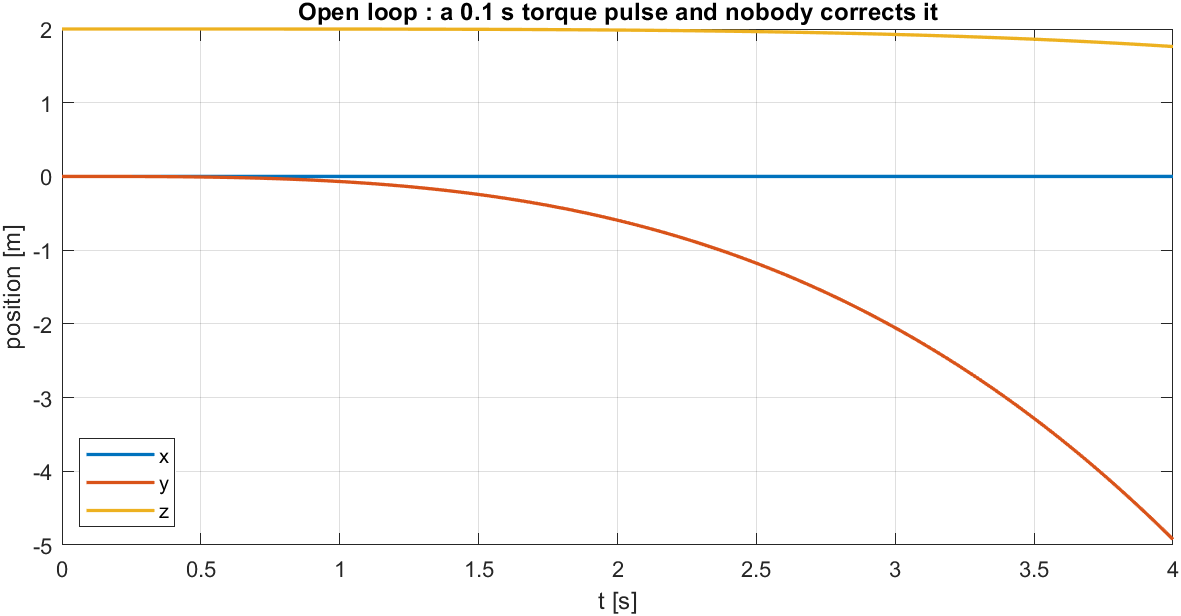
\includegraphics[width=0.62\linewidth]{M1_1_Dynamics_Linearization_1.png}
  \caption{Open loop: a 0.1\,s torque pulse and no correction. The drone slides further and further away.}
  \label{fig:openloop}
\end{figure}

\begin{real}
Equations (1)--(4) are ``the real drone''. In our setup Gazebo solves them for the Iris quadrotor; we never solve them
in the controller. Our node only \emph{reads} their result. The position and the attitude arrive on
\code{/ap/v1/pose/filtered}; the attitude comes as a quaternion and is turned into the rotation matrix $R$:
\pyfile{371}{386}{\node}{drones\_controller/controller\_node.py --- pose\_callback()}
\pyfile{24}{40}{\sad}{drones\_controller/state\_adapter.py --- quaternion\_to\_rotation\_matrix(): the matrix $R$}
The node also checks that this really is a rotation matrix ($R^\top R=I$, $\det R=1$), the two properties of
\cref{sec:rotations}:
\pyfile{127}{138}{\sad}{drones\_controller/state\_adapter.py --- validate\_rotation\_matrix()}
\end{real}

% ---------------------------------------------------------------------
\subsection{Block 2 --- Linearization: zooming in on the dynamics}
\label{sec:m1b2}
% ---------------------------------------------------------------------

\begin{idea}
Equations (1)--(4) are curved (nonlinear): they contain $R$, products and sines. But if we zoom in close to one
flight condition, any smooth curve looks like a straight line (\cref{sec:taylor}). Near that condition the drone
behaves like a simple \emph{linear} system, and linear systems are easy to predict and to control. The ``slopes'' of
this straight-line model are two matrices, $A$ and $B$.
\end{idea}

\begin{eqbox}{Equations (5)--(6): first order Taylor expansion and the Jacobians}
\begin{align}
  \vf(\vx,\vu) &\approx \vf(\hx,\hat\vu) + A\,\delta\vx + B\,\delta\vu \tag{5}\label{eq:5}\\
  A &= \left.\frac{\partial\vf}{\partial\vx}\right|_{\hx,\hat\vu}\in\R^{12\times12},\qquad
  B = \left.\frac{\partial\vf}{\partial\vu}\right|_{\hx,\hat\vu}\in\R^{12\times4} \tag{6}\label{eq:6}
\end{align}
with the 12-number error $\delta\vx=[\delta\vp;\ \delta\vv;\ \delta\vth;\ \delta\vw]$, where $R=\hR\,\Exp(\delta\vth)$, and $\delta\vu=\vu-\hat\vu$.
\end{eqbox}

\subsubsection*{What is $\delta\vx$?}
$\delta\vx$ is ``the difference between the true state and a reference state'' (later: the estimate).
For position, velocity and angular velocity this is a simple subtraction: $\delta\vp=\vp-\hp$ and so on. For the
attitude we cannot subtract matrices (the result would not be a rotation). Instead we ask: ``which small rotation
$\delta\vth$ takes $\hR$ to $R$?'', i.e.\ $R=\hR\,\Exp(\delta\vth)$, so $\delta\vth=\Log(\hR^\top R)$. That is 3
numbers. So $\delta\vx$ has $3+3+3+3=12$ numbers.

\subsubsection*{Deriving $A$ and $B$, one row at a time}
Put $\vp=\hp+\delta\vp$, $\vv=\hv+\delta\vv$, $R\approx\hR(I+\skw{\delta\vth})$, $\vw=\hw+\delta\vw$,
$T=\hat T+\delta T$, $\vtau=\hat\vtau+\delta\vtau$ into (1)--(4). Keep every term that contains \emph{one} small
quantity and throw away products of two small quantities (they are tiny squared).

\textbf{Position row.} $\dot\vp=\vv$ gives $\delta\dot{\vp}=\delta\vv$ directly.

\textbf{Velocity row.}
$\dot{\vv}\approx\vg+\frac{\hat T+\delta T}{m}\hR(I+\skw{\delta\vth})\ve_3$. Multiply out and subtract the reference
part $\vg+\frac{\hat T}{m}\hR\ve_3$:
\[
\delta\dot\vv=\frac{\hat T}{m}\hR\skw{\delta\vth}\ve_3+\frac{\delta T}{m}\hR\ve_3+\underbrace{\tfrac{\delta T}{m}\hR\skw{\delta\vth}\ve_3}_{\text{two small terms: drop}} .
\]
Using $\skw{\delta\vth}\ve_3=\delta\vth\times\ve_3=-\ve_3\times\delta\vth=-\skw{\ve_3}\delta\vth$:
\[
\delta\dot{\vv}=-\frac{\hat T}{m}\hR\skw{\ve_3}\,\delta\vth+\frac{1}{m}\hR\ve_3\,\delta T .
\]

\textbf{Attitude row.} Both $R$ and $\hR$ follow (3). Differentiating $R=\hR\Exp(\delta\vth)$ and keeping first order
terms gives
\[
\delta\dot{\vth}=-\skw{\hw}\,\delta\vth+\delta\vw .
\]
In words: an angular-velocity error makes the attitude error grow; the first term just accounts for the reference
frame itself spinning.

\textbf{Angular-velocity row.} The only nonlinear part of (4) is $\vw\times J\vw$. Its derivative with respect to $\vw$
is $\skw{\vw}J-\skw{J\vw}$ (product rule for the cross product), so
\[
\delta\dot{\vw}=J^{-1}\big(\skw{J\hw}-\skw{\hw}J\big)\delta\vw+J^{-1}\delta\vtau .
\]

Stacking the four rows (each block is $3\times3$; the columns follow $\delta\vp,\delta\vv,\delta\vth,\delta\vw$ for $A$
and $\delta T,\delta\vtau$ for $B$):
\begin{equation}
\label{eq:AB}\tag{6a}
A=\begin{bmatrix}
0&I&0&0\\
0&0&-\frac{\hat T}{m}\hR\skw{\ve_3}&0\\
0&0&-\skw{\hw}&I\\
0&0&0&J^{-1}\big(\skw{J\hw}-\skw{\hw}J\big)
\end{bmatrix},\qquad
B=\begin{bmatrix}0&0\\ \frac1m\hR\ve_3&0\\ 0&0\\ 0&J^{-1}\end{bmatrix}.
\end{equation}

\begin{toy}[the Jacobians at hover, and how good ``first order'' is]
At hover ($\hR=I$, $\hw=0$, $\hat T=mg_0$) the important blocks are
\[
-g_0\skw{\ve_3}=\begin{bmatrix}0&9.81&0\\-9.81&0&0\\0&0&0\end{bmatrix},\qquad
\tfrac1m\ve_3=\begin{bmatrix}0\\0\\0.667\end{bmatrix},\qquad
J^{-1}=\diag(50,\,50,\,25).
\]
Read them as sentences:
\begin{itemize}
  \item a pitch error of $\delta\theta_y$ radians accelerates the drone along $+x$ at $9.81\,\delta\theta_y$\,m/s$^2$
        (row 1 of the first matrix); a roll error accelerates it along $-y$ (row 2);
  \item 1\,N of extra thrust gives 0.667\,m/s$^2$ of extra \emph{vertical} acceleration and nothing else;
  \item 1\,N\,m of roll torque gives 50\,rad/s$^2$ of roll acceleration.
\end{itemize}
\textbf{Check by numbers.} The toy model also computes the derivatives numerically, $(\vf(\vx+h)-\vf(\vx-h))/2h$,
at a tilted, spinning, climbing state. The largest difference from the formulas is $4.9\times10^{-10}$ for $A$ and
$6.8\times10^{-10}$ for $B$: the derivation is right.

\textbf{How far can we trust the straight line?} Pitch the hovering drone by $\theta$. The linear model says
$\dot v_x=g_0\theta$, the truth is $g_0\sin\theta$ (the $\sin$ example of \cref{sec:taylor}):
\begin{center}\small
\begin{tabular}{rrrr}
\toprule
$\theta$ [deg] & linear $g_0\theta$ [m/s$^2$] & true $g_0\sin\theta$ [m/s$^2$] & error\\
\midrule
1 & 0.1712 & 0.1712 & 0.005\%\\
2.87 & 0.4914 & 0.4912 & 0.04\%\\
10 & 1.7122 & 1.7035 & 0.51\%\\
20 & 3.4243 & 3.3552 & 2.06\%\\
28.65 & 4.9054 & 4.7035 & 4.29\%\\
\bottomrule
\end{tabular}
\end{center}
In normal flight the tilt stays below 10$^\circ$, where the linear model is better than 0.5\%.
\end{toy}

\begin{toycode}{M1\_1\_Dynamics\_Linearization}{Block 2}
[A, B] = DroneLib.jacobians(x_hover, u_hover, P);
A_v_theta = A(4:6, 7:9)      % a pitch error pushes along +x, a roll error along -y
B_v_T     = B(4:6, 1)'       % extra thrust only changes vertical acceleration (1/m)
B_w_tau   = B(10:12, 2:4)    % torque -> angular acceleration (J^-1)
\end{toycode}

\begin{real}
Our Python node does not compute $A$ and $B$; they are used \emph{inside the estimator} (block 4), which in our
SITL setup is ArduPilot's EKF3. They are also the reason Model~2 can use a linear model at all: the table above shows
that near hover the drone really is almost linear. And they are what Model~2 learns from data
(\cref{sec:m2b2}): DMDc recovers these same numbers without knowing $m$ or $J$.
\end{real}

% ---------------------------------------------------------------------
\subsection{Block 3 --- How a small error grows (local error dynamics)}
\label{sec:m1b3}
% ---------------------------------------------------------------------

\begin{idea}
Suppose our belief about the drone is slightly wrong. How does that mistake change over time if we only trust the
physics? Block 3 answers this with the linear model of block 2. This is exactly what the estimator needs to know to
decide how much it can still trust its own prediction.
\end{idea}

\begin{eqbox}{Equations (7)--(9): linear dynamics of the error}
\begin{align}
  \delta\vx &= \big[\vp-\hp;\ \vv-\hv;\ \Log(\hR^\top R);\ \vw-\hw\big] \tag{7}\label{eq:7}\\
  \delta\dot{\vx} &= A\,\delta\vx + B\,\delta\vu \tag{8}\label{eq:8}\\
  \delta\vx_{k+1} &= F\,\delta\vx_k + G\,\delta\vu_k,\qquad F=e^{A\Delta t}\approx I+A\Delta t,\quad G\approx B\Delta t \tag{9}\label{eq:9}
\end{align}
\end{eqbox}

\subsubsection*{Derivation}
The truth follows $\dot\vx=\vf(\vx,\vu)$ and the estimate follows the same model, $\dot\hx=\vf(\hx,\hat\vu)$.
Subtract the two and use (5):
\[
\delta\dot\vx=\vf(\vx,\vu)-\vf(\hx,\hat\vu)\approx\big[\vf(\hx,\hat\vu)+A\delta\vx+B\delta\vu\big]-\vf(\hx,\hat\vu)=A\delta\vx+B\delta\vu .
\]
The big nonlinear parts cancel; only the small linear error is left. That is (8).

For a computer we need one time step $\Delta t$. The exact solution of $\delta\dot\vx=A\delta\vx$ over one step is
$\delta\vx_{k+1}=e^{A\Delta t}\delta\vx_k$, where the matrix exponential is the series
$e^{A\Delta t}=I+A\Delta t+\frac12(A\Delta t)^2+\dots$ (Taylor again). Keeping the first two terms gives
$F\approx I+A\Delta t$, which is the same as one Euler step.

\textbf{Why a drone drifts away.} At hover every eigenvalue of $A$ is 0. Look at the chain inside $A$:
angular-velocity error $\to$ attitude error $\to$ velocity error $\to$ position error. Each arrow is an
integration. A constant roll-rate error $\delta\omega_x$ therefore becomes
$\delta\theta_x=\delta\omega_x t$, then $\delta v_y=-g_0\delta\omega_x t^2/2$, then
\[
\delta y(t)=-\frac{g_0\,\delta\omega_x\,t^3}{6}.
\]
\begin{toy}[a tiny gyro error becomes a big position error]
$\delta\omega_x=0.01$\,rad/s (about half a degree per second, a typical gyro bias). After 2\,s:
$\delta y=-9.81\times0.01\times8/6=-0.131$\,m. After 5\,s: $-2.04$\,m. After 10\,s: $-16.4$\,m. This $t^3$ growth is why an
IMU on its own is useless for position after a few seconds, and why the camera is needed.

\textbf{Linear prediction versus truth.} The toy model starts the drone with an initial error (10\,cm, 0.2\,rad/s of
yaw rate, and a roll error) and compares the linear prediction $e^{At}\delta\vx_0$ with the true nonlinear motion over
2\,s. With a 2$^\circ$ roll error they differ by only 0.02\%; with a 30$^\circ$ roll error the linear model is off
by 4.7\% (\cref{fig:errgrow}). The linear model is \emph{local}: perfect for small errors, worse for large ones.

\textbf{One-step check.} With $\Delta t=0.01$\,s, the biggest entry of $F-e^{A\Delta t}$ is $4.9\times10^{-4}$,
the size of the dropped $\tfrac12(A\Delta t)^2$ term. So $F=I+A\Delta t$ is good enough.
\end{toy}

\begin{figure}[H]
  \centering
  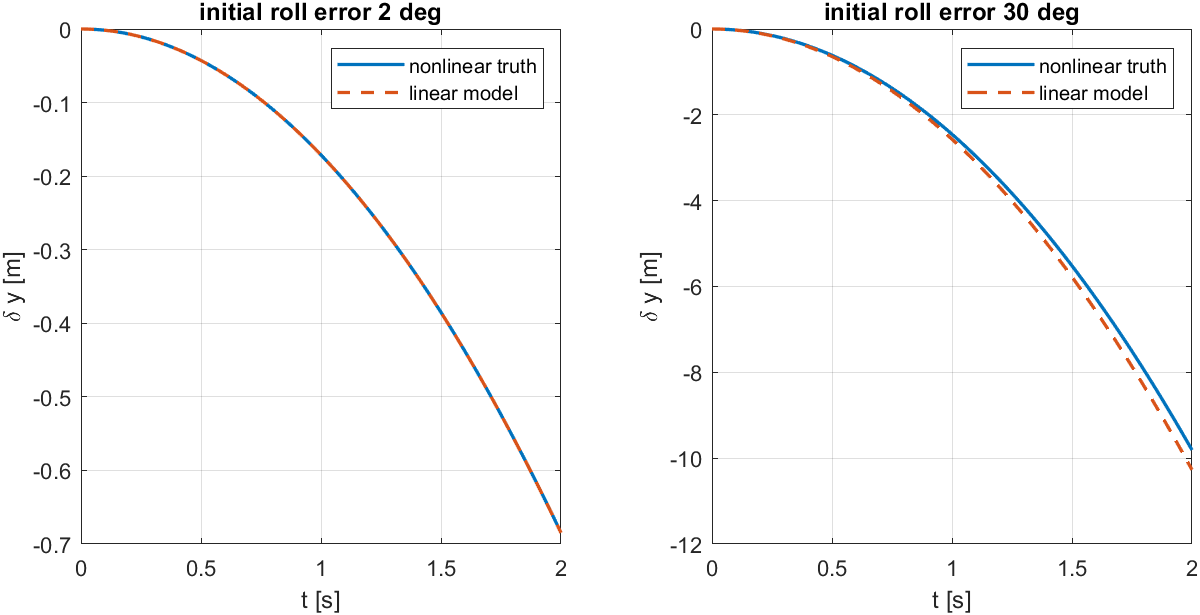
\includegraphics[width=0.85\linewidth]{M1_1_Dynamics_Linearization_2.png}
  \caption{Sideways error $\delta y$ after an initial roll error: nonlinear truth (solid) and linear model (dashed).}
  \label{fig:errgrow}
\end{figure}

\begin{toycode}{M1\_1\_Dynamics\_Linearization}{Block 3}
dt = 0.01;                          % EKF / IMU sample time [s]
F  = eye(12) + A*dt;
max_F_error = max(abs(F - expm(A*dt)), [], 'all')   % size of the dropped (A dt)^2/2
eig_A = eig(A)'                                       % all zero at hover
\end{toycode}

\begin{real}
The estimator never tries to describe the whole flight with a linear model. It only describes the \emph{small
difference} between what it believes and what is true, and that difference stays small because the camera and the
IMU keep correcting it. That is why the filter of block~4 is called an \emph{error-state} filter, and why $F$ is all
it needs.
\end{real}

% ---------------------------------------------------------------------
\subsection{Block 4 --- Where am I? The error-state Kalman filter (our VIO)}
\label{sec:m1b4}
% ---------------------------------------------------------------------

\begin{idea}
We have two imperfect sources of information. The \emph{physics} (blocks 1--3) predicts where the drone should be,
but small mistakes grow quickly. The \emph{sensors} tell us where it is, but every reading is noisy, and the camera
only gives a new reading 25 times a second. The Kalman filter combines them in the best possible way. It repeats
two steps for ever:
\begin{enumerate}
  \item \textbf{Predict.} ``I know how I pushed the drone, so physics tells me where it should be now.'' The guess
        moves forward, and because physics is never perfect, the uncertainty \emph{grows}.
  \item \textbf{Correct.} ``A sensor reading arrived. How surprised am I?'' The guess moves towards the reading. How
        far depends on whom we trust more. The uncertainty \emph{shrinks}.
\end{enumerate}
The filter remembers two things: the \textbf{estimate} $\hx_k$ (its best guess) and the \textbf{covariance} $P_k$
(a $12\times12$ matrix that says how unsure it is in each of the 12 error directions).
\end{idea}

\begin{eqbox}{Equations (10)--(14): error-state extended Kalman filter}
\textbf{Prediction (every IMU sample, 100\,Hz)}
\begin{align}
  \hx_{k+1} &= \vf_d(\hx_k,\vu_k) \tag{10}\label{eq:10}\\
  P_{k+1}   &= F P_k F^\top + Q \tag{11}\label{eq:11}
\end{align}
\textbf{Correction (whenever a measurement $\vz$ arrives)}
\begin{align}
  K   &= P H^\top\big(HPH^\top+R_n\big)^{-1} \tag{12}\label{eq:12}\\
  \delta\hat{\vx} &= K\big(\vz-h(\hx)\big),\quad
  \hp\leftarrow\hp+\delta\hat{\vp},\ \hv\leftarrow\hv+\delta\hat{\vv},\ \hR\leftarrow\hR\,\Exp(\delta\hat{\vth}),\ \hw\leftarrow\hw+\delta\hat{\vw} \tag{13}\label{eq:13}\\
  P   &\leftarrow (I-KH)\,P \tag{14}\label{eq:14}
\end{align}
$\vf_d$ = one simulation step of (1)--(4); $Q$ = how much the physics may be wrong per step (wind, model errors);
$\vz$ = measurement; $h(\hx)$ = what we expect to measure if our estimate were right; $H$ = Jacobian of $h$;
$R_n$ = covariance of the sensor noise; $K$ = Kalman gain.
\end{eqbox}

\subsubsection*{First understand it with one number}
Before matrices, take a single quantity, the altitude $z$, with a guess $\hat z$ and variance $P$.

\textbf{Predict.} If we command a climb of $c$\,m/s for $\Delta t$ seconds, the guess becomes $\hat z+c\Delta t$. The old
uncertainty is still there, and the physics adds a bit more ($Q$): $P^-=P+Q$.

\textbf{Correct.} A sensor reads $z_m$ with noise variance $R_n$. The surprise (the \textbf{innovation}) is
$r=z_m-\hat z^-$. We move a fraction $K$ of the surprise: $\hat z^+=\hat z^-+K\,r$. Which fraction is best? The new
error is $(1-K)\times$(old error) $-K\times$(sensor noise), whose variance is
\[
P^+=(1-K)^2P^-+K^2R_n .
\]
This is a bowl in $K$ (\cref{sec:minquad}). Set the slope to zero:
$-2(1-K)P^-+2KR_n=0\Rightarrow K=\dfrac{P^-}{P^-+R_n}$. Putting it back gives $P^+=(1-K)P^-$.

So $K$ is simply ``my uncertainty divided by (my uncertainty + the sensor's uncertainty)''. If I am very unsure
($P^-$ large), $K\to1$ and I believe the sensor. If the sensor is very noisy ($R_n$ large), $K\to0$ and I ignore it.

\begin{toy}[one predict and one correct, altitude only]
Prior: $\hat z_k=10$\,m with $P_k=3.5$\,m$^2$. We command a climb of 0.5\,m/s for 1\,s, $F=1$, $Q=0.5$:
\[
\hat z^-=10+0.5=10.5\ \text{m},\qquad P^-=1\cdot3.5\cdot1+0.5=4.0\ \text{m}^2 .
\]
A sensor reads $z=12.5$\,m with $R_n=1$\,m$^2$ and $H=1$:
\[
K=\frac{4.0}{4.0+1}=0.8,\qquad \hat z^+=10.5+0.8\,(12.5-10.5)=12.1\ \text{m},\qquad P^+=(1-0.8)\cdot4.0=0.8\ \text{m}^2 .
\]
The sensor is four times more trustworthy than the prediction ($4.0$ versus $1$), so the estimate moves 80\% of the
way towards it, and the variance drops from 4.0 to 0.8. Both sources together are better than either alone.
\end{toy}

\begin{toycode}{M1\_2\_Error\_State\_EKF}{Toy example - altitude only}
z_hat = 10;  Pk = 3.5;  F = 1;  Q = 0.5;  climb = 0.5;  dt = 1;
z_hat = z_hat + climb*dt          % predict the guess
Pk    = F*Pk*F' + Q               % uncertainty grows
z = 12.5;  H = 1;  Rn = 1;
K     = Pk*H'/(H*Pk*H' + Rn)      % how much to trust the sensor
z_hat = z_hat + K*(z - H*z_hat)   % corrected guess
Pk    = (1 - K*H)*Pk              % uncertainty shrinks
\end{toycode}

\subsubsection*{The same thing with matrices}
Now the error is the 12-vector $\delta\vx$ and the uncertainty is the matrix $P$.

\textbf{(10) Predict the guess.} The best guess of the next state is to run the full nonlinear physics one step
forward from the current guess with the input we applied. The error we do not know averages to zero, so it does not
move the guess.

\textbf{(11) Predict the uncertainty.} From block 3, the error moves as $\delta\vx_{k+1}=F\delta\vx_k+\bm w_k$, where
$\bm w_k$ is the new random error added by the wind and by model mistakes, with covariance $Q$. Using the rule
$P'=FPF^\top$ of \cref{sec:maths} and the fact that $\bm w_k$ is independent of the old error:
\[
P_{k+1}=\mathbb E[\delta\vx_{k+1}\delta\vx_{k+1}^\top]=F\,P_k\,F^\top+Q .
\]
Uncertainty is stretched by the physics ($FPF^\top$) and inflated by the noise ($+Q$).

\textbf{(12) The Kalman gain.} A sensor does not see the whole state. A camera sees position and attitude; a gyro
sees angular velocity. $H$ picks out what the sensor sees: the innovation is $\vr=\vz-h(\hx)\approx H\delta\vx+\bm v$
(``what I see minus what I expected = my error seen through the sensor + sensor noise''). Correcting by
$\delta\hat\vx=K\vr$ leaves the error $(I-KH)\delta\vx-K\bm v$ with covariance
\[
P^+=(I-KH)P(I-KH)^\top+KR_nK^\top .
\]
Exactly as in the one-number case, we choose $K$ to make the total uncertainty (the sum of the diagonal, the trace)
as small as possible. Setting the derivative with respect to $K$ to zero:
\[
-2PH^\top+2K\big(HPH^\top+R_n\big)=0\quad\Longrightarrow\quad K=PH^\top\big(HPH^\top+R_n\big)^{-1}.
\]
Compare with $K=P^-/(P^-+R_n)$: it is the same formula, with matrices.

\textbf{(13) Correct the guess.} $\delta\hat\vx=K\vr$ is our best estimate of the error, so we add it to the guess.
Position, velocity and angular velocity are added normally. The attitude is \emph{rotated}: $\hR\leftarrow\hR\Exp(\delta\hat\vth)$,
so $\hR$ stays a true rotation matrix. This is the ``error-state'' trick: the filter works with a small 3-number
attitude error and never adds matrices that should be rotations.

\textbf{(14) Shrink the uncertainty.} Putting the best $K$ into the expression for $P^+$ simplifies it to
$P^+=(I-KH)P$.

\subsubsection*{Our sensors}
\begin{center}\small
\begin{tabular}{@{}llll@{}}
\toprule
Sensor (rate) & innovation $\vr$ & $H$ & noise $\sigma$\\
\midrule
Gyroscope (100\,Hz) & $\tilde{\vw}-\hw$ & $[\,0\ \ 0\ \ 0\ \ I\,]$ & 0.01\,rad/s\\
Camera / VIO (25\,Hz) & $\begin{bmatrix}\tilde{\vp}-\hp\\ \Log(\hR^\top\tilde R)\end{bmatrix}$ &
  $\begin{bmatrix}I&0&0&0\\0&0&I&0\end{bmatrix}$ & 5\,cm, 0.02\,rad\\
\bottomrule
\end{tabular}
\end{center}
Each block of $H$ is $3\times3$, in the order $[\delta\vp,\delta\vv,\delta\vth,\delta\vw]$. The \textbf{velocity is never
measured}. The filter works it out from how the measured position changes, through the physics in $F$.

\begin{toy}[the full 12-state filter on the drone (\code{M1\_2})]
The drone flies a climbing helix in gusty wind for 20\,s. The filter starts with a wrong guess (30\,cm, 0.2\,m/s and
about 7$^\circ$ off) and sees only the commands and the noisy sensors. After the first 2\,s:
\begin{center}\small
\begin{tabular}{lrl}
\toprule
quantity & estimation error (RMS) & for comparison\\
\midrule
position & 2.55\,cm & the camera alone: 8.55\,cm\\
velocity (never measured!) & 3.85\,cm/s & --\\
attitude & 0.20$^\circ$ & camera noise: 1.15$^\circ$\\
\bottomrule
\end{tabular}
\end{center}
The fused estimate is more than three times better than the camera alone. In 99\% of the samples all 12 errors lie
inside the $\pm3\sigma$ band that the filter itself predicts from $P_k$: the filter knows how unsure it is.
\end{toy}

\begin{figure}[H]
  \centering
  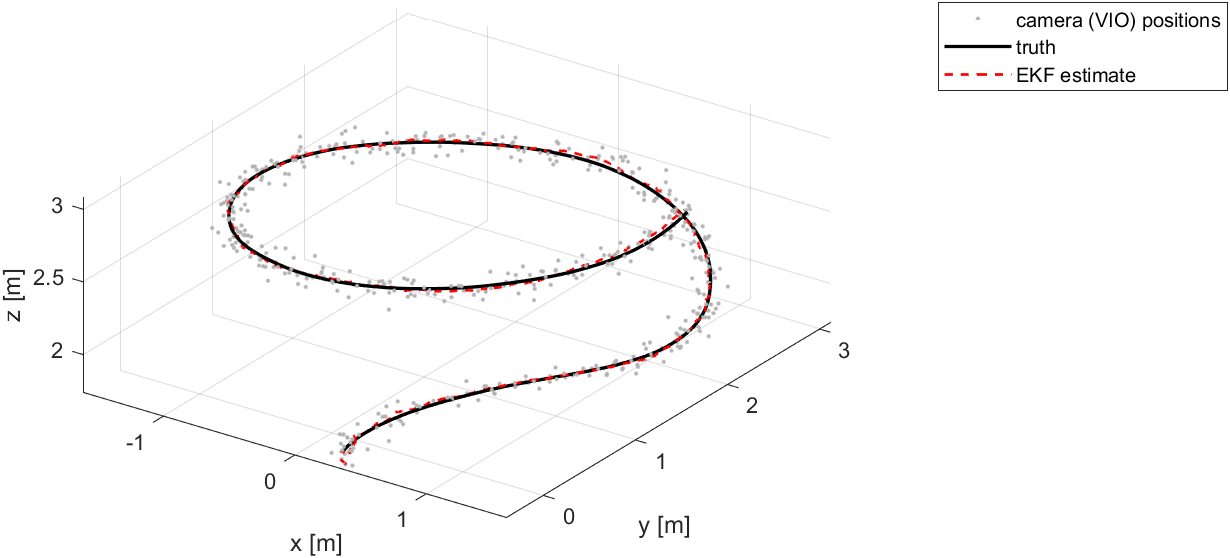
\includegraphics[width=0.8\linewidth]{M1_2_Error_State_EKF_1.png}\\[4pt]
  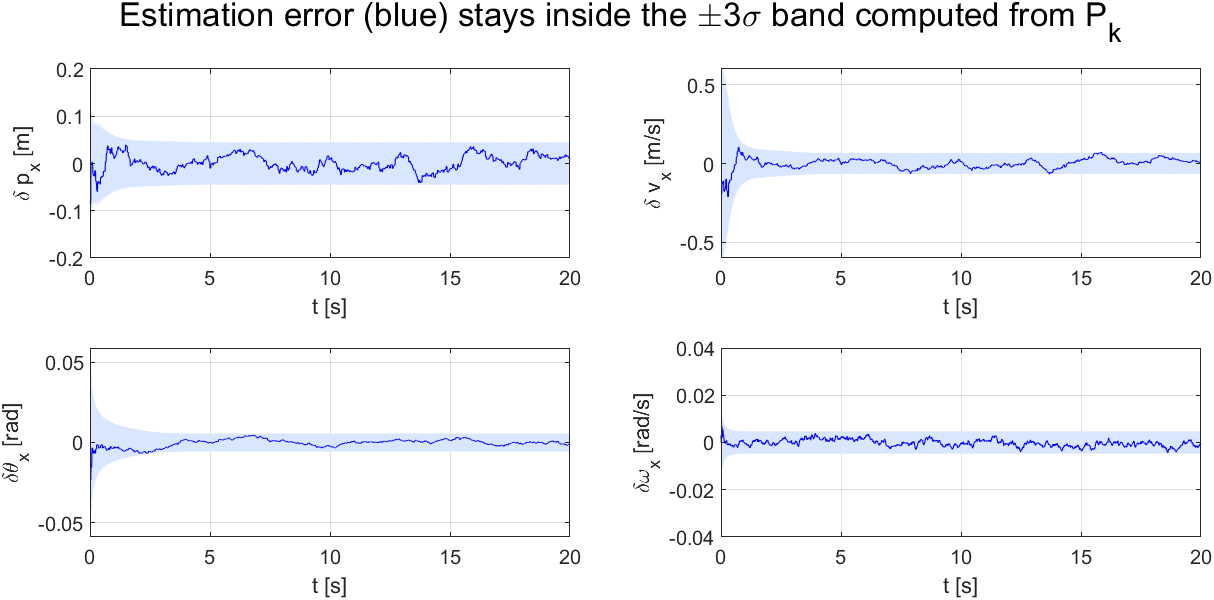
\includegraphics[width=0.9\linewidth]{M1_2_Error_State_EKF_2.png}
  \caption{Top: noisy camera positions (grey dots), truth (black) and EKF estimate (red, dashed). Bottom: estimation
  errors (blue) stay inside the $\pm3\sigma$ band computed from $P_k$.}
\end{figure}

\begin{toycode}{M1\_2\_Error\_State\_EKF}{Run the filter}
for k = 1:N
    [~, ~, ~, wh] = DroneLib.unpack(xh);                       % gyro correction
    [xh, Pk] = DroneLib.ekf_update(xh, Pk, Zg(:,k) - wh, Hg, Rg);
    if mod(k-1, 4) == 0                                % camera (25 Hz)
        [ph, ~, Rh] = DroneLib.unpack(xh);
        r = [Zp(:,k) - ph; DroneLib.logSO3(Rh'*DroneLib.expSO3(Zth(:,k)))];
        [xh, Pk] = DroneLib.ekf_update(xh, Pk, r, Hc, Rc);
    end
    ...
    [xh, Pk] = DroneLib.ekf_predict(xh, Pk, U(:,k), dt, P, Q);  % prediction
end
\end{toycode}
\begin{lstlisting}[style=mat, title={\small\sffamily toy\_model3/DroneLib.m --- ekf\_predict and ekf\_update, equations (9)--(14)}]
A  = DroneLib.jacobians(xh, u, P);
F  = eye(12) + A*dt;                                 % (9)
xh = DroneLib.rk4(xh, u, dt, P);                     % (10)
Pk = F*Pk*F' + Q;                                    % (11)

K  = Pk*H' / (H*Pk*H' + Rn);                         % (12)
xh = DroneLib.boxplus(xh, K*r);                      % (13)  R <- R*Exp(dtheta)
Pk = (eye(12) - K*H)*Pk;                             % (14)
\end{lstlisting}

\begin{real}[this is the ``VIO'' of our title]
A monocular camera alone cannot tell scale (a small room close up looks like a big room far away) and an IMU alone
drifts within seconds ($t^3$, block 3). The Kalman filter is the referee that fuses them. Between camera frames it
predicts with the physics and the gyro; when a frame arrives, the visual-odometry pose corrects the prediction, and
$K$ decides how much to trust each source.

In our SITL setup this filter runs \emph{inside ArduPilot} (its EKF3 has exactly this predict / correct structure,
with more states such as sensor biases). Its output arrives on \code{/ap/v1/pose/filtered} and
\code{/ap/v1/twist/filtered}. Our node stores it, and before every control step checks that the estimate is complete,
recent and finite:
\pyfile{447}{480}{\node}{drones\_controller/controller\_node.py --- state\_is\_valid() (first part)}
If the estimate is older than \code{state\_timeout} = 0.5\,s, the controller does nothing at all. This is a safety rule:
never fly on stale information.
\end{real}

% ---------------------------------------------------------------------
\subsection{Block 5 --- Position control (outer loop)}
\label{sec:m1b5}
% ---------------------------------------------------------------------

\begin{idea}
Compare where we are with where we should be, and ask for an acceleration that pulls us there: the further away,
the harder we pull (a spring), and the faster we are already moving towards the target, the less we pull (a damper).
\end{idea}

\begin{eqbox}{Equations (15)--(16): tracking errors and desired acceleration}
\begin{align}
  \ve_p=\vp_d-\hp,\qquad \ve_v&=\vv_d-\hv \tag{15}\label{eq:15}\\
  \va_d&=\ddot{\vp}_d+K_p\,\ve_p+K_v\,\ve_v \tag{16}\label{eq:16}
\end{align}
$\vp_d,\vv_d,\ddot\vp_d$: desired position, velocity, acceleration. $K_p,K_v$: diagonal gain matrices.
\end{eqbox}

\subsubsection*{Why this works: a spring and a damper}
Suppose the inner loops deliver exactly the acceleration we ask for, $\ddot{\vp}=\va_d$. Then the position error
$\ve_p=\vp_d-\vp$ changes as
\[
\ddot{\ve}_p=\ddot{\vp}_d-\ddot{\vp}=\ddot{\vp}_d-\va_d=-K_p\ve_p-K_v\dot{\ve}_p
\quad\Longrightarrow\quad \ddot{\ve}_p+K_v\dot{\ve}_p+K_p\ve_p=\bm0 .
\]
This is the equation of a mass on a spring (stiffness $k_p$) with a damper (friction $k_v$), one per axis. Its
solutions behave like $e^{st}$ with $s^2+k_vs+k_p=0$. If $k_p>0$ and $k_v>0$, both roots have negative real part, so the
error always dies out. Comparing with the standard form $s^2+2\zeta\omega_ns+\omega_n^2$:
\[
\omega_n=\sqrt{k_p}\ \text{(how fast)},\qquad \zeta=\frac{k_v}{2\sqrt{k_p}}\ \text{(how damped)},\qquad t_{\text{settle}}\approx\frac{4}{\zeta\omega_n}.
\]
\begin{center}\small
\begin{tabular}{@{}lrrrrr@{}}
\toprule
axis & $k_p$ & $k_v$ & $\omega_n$ [rad/s] & $\zeta$ & $t_{\text{settle}}$ [s]\\
\midrule
$x,\ y$ & 1.5 & 1.2 & 1.225 & 0.490 & 6.7\\
$z$ & 2.0 & 1.5 & 1.414 & 0.530 & 5.3\\
\bottomrule
\end{tabular}
\end{center}
Our \code{controller.yaml} gains are gentle: $\zeta\approx0.5$ means a small overshoot, and the error settles in
about 6\,s. That suits a camera drone that should move smoothly. The term $\ddot{\vp}_d$ (``feed-forward'') supplies the
acceleration a perfect pilot would need to follow a moving target; the feedback terms only fix what is left over.

\begin{toy}[50 cm too low and already climbing]
Setpoint $\vp_d=[0,0,2]$\,m (the \code{controller.yaml} hover point), $\vv_d=\ddot{\vp}_d=\bm0$. The estimator says
$\hp=[0.1,\,-0.2,\,1.5]$\,m and $\hv=[0,0,0.3]$\,m/s.
\[
\ve_p=\begin{bmatrix}0-0.1\\0-(-0.2)\\2-1.5\end{bmatrix}=\begin{bmatrix}-0.1\\0.2\\0.5\end{bmatrix},\quad
\ve_v=\begin{bmatrix}0\\0\\-0.3\end{bmatrix},\quad
\va_d=\begin{bmatrix}1.5(-0.1)\\1.5(0.2)\\2(0.5)+1.5(-0.3)\end{bmatrix}=\begin{bmatrix}-0.15\\0.30\\0.55\end{bmatrix}\text{ m/s}^2 .
\]
It is 50\,cm low, so it wants to accelerate up. Because it is already climbing at 0.3\,m/s, it asks for less: 0.55
instead of 1.0. That is the damper at work, preventing overshoot.
\end{toy}

\begin{toycode}{M1\_3\_SO3\_Control\_Closed\_Loop}{Block 5}
p_hat = [0.1; -0.2; 1.5];   v_hat = [0; 0; 0.3];
p_d   = [0; 0; 2];          v_d = [0; 0; 0];     a_ff = [0; 0; 0];
e_p = p_d - p_hat
e_v = v_d - v_hat
a_d = a_ff + P.Kp*e_p + P.Kv*e_v
\end{toycode}

\begin{real}
Equation (15) is \code{compute\_position\_errors()} and equation (16) is the first part of
\code{compute\_desired\_force()} in our controller (\code{a\_cmd} is $\va_d$):
\pyfile{32}{40}{\so}{drones\_controller/so3\_controller.py --- equation (15)}
\pyfile{64}{68}{\so}{drones\_controller/so3\_controller.py --- equation (16)}
The desired state comes from \code{WaypointGenerator}: a fixed point $[0,0,2]$ with $\vv_d=\va_d=\bm0$, read from the YAML.
\end{real}

% ---------------------------------------------------------------------
\subsection{Block 6 --- Force and attitude: which way to lean}
\label{sec:m1b6}
% ---------------------------------------------------------------------

\begin{idea}
A quadrotor can only push along its own up-axis. To get the acceleration $\va_d$ it must (1) work out the total force
needed, including holding up its own weight, and (2) tilt so that its up-axis points along that force. Like a person
pushing a heavy cart: to push forward, you lean forward.
\end{idea}

\begin{eqbox}{Equations (17)--(19): desired force, thrust direction and attitude}
\begin{align}
  \vF_d &= m\,(\va_d-\vg) \tag{17}\label{eq:17}\\
  \vb_{3d} &= \frac{\vF_d}{\|\vF_d\|} \tag{18}\label{eq:18}\\
  \vb_{1c}=[\cos\psi_d,\ \sin\psi_d,\ 0]^\top,\quad
  \vb_{2d}&=\frac{\vb_{3d}\times\vb_{1c}}{\|\vb_{3d}\times\vb_{1c}\|},\quad
  \vb_{1d}=\vb_{2d}\times\vb_{3d},\quad
  R_d=\big[\vb_{1d}\ \ \vb_{2d}\ \ \vb_{3d}\big] \tag{19}\label{eq:19}
\end{align}
\end{eqbox}

\subsubsection*{Derivation}
\textbf{(17)} We want $\dot\vv=\va_d$. Equation (2) says $\dot\vv=\vg+\frac{T}{m}R\ve_3$, so the thrust vector must be
$T\,R\ve_3=m(\va_d-\vg)$. Call this $\vF_d$. Because $\vg$ points down, $-\vg$ points up: even for $\va_d=0$ the drone
must push up with $mg_0=14.7$\,N.

\textbf{(18)} $T R\ve_3=T\vb_3$ is a vector of length $T$ along the drone's up-axis. For it to equal $\vF_d$, the up-axis
must point along $\vF_d$, so $\vb_{3d}=\vF_d/\|\vF_d\|$, and the thrust must be $T=\|\vF_d\|$.
This is the key fact of quadrotor flight: \emph{position is controlled through the attitude}.

\textbf{(19)} $\vb_{3d}$ fixes the tilt (two of the three rotation directions). The third, yaw (where the nose points),
is our free choice $\psi_d$. We build the remaining two axes so that they are unit length and at right angles:
\begin{itemize}
  \item $\vb_{1c}$ is the heading we would like, flat on the ground.
  \item $\vb_{2d}=\vb_{3d}\times\vb_{1c}$ (normalised) is at right angles to both the up-axis and the heading: the drone's ``left''.
  \item $\vb_{1d}=\vb_{2d}\times\vb_{3d}$ is at right angles to both: the nose, as close to the wanted heading as the tilt allows.
\end{itemize}
The three columns are orthonormal and right-handed, so $R_d^\top R_d=I$ and $\det R_d=1$: $R_d$ is a true rotation.
The construction only fails if $\vb_{3d}$ is parallel to $\vb_{1c}$ (a 90$^\circ$ tilt); the code then nudges the yaw.

\begin{toy}[continuing the example of block 5]
$\va_d=[-0.15,\,0.30,\,0.55]$, $m=1.5$, $\vg=[0,0,-9.81]$, $\psi_d=0$:
\[
\vF_d=1.5\,[-0.15,\ 0.30,\ 0.55+9.81]=[-0.225,\ 0.450,\ 15.540]\ \text{N},\qquad \|\vF_d\|=15.548\ \text{N},
\]
\[
\vb_{3d}=[-0.0145,\ 0.0289,\ 0.9995],\qquad
R_d=\begin{bmatrix}0.9999&0.0000&-0.0145\\0.0004&0.9996&0.0289\\0.0145&-0.0289&0.9995\end{bmatrix}.
\]
Tilt $=\arccos(0.9995)=1.85^\circ$: lean very slightly towards $-x$ and $+y$ (where the target is) and push 15.5\,N,
more than the 14.7\,N weight because the drone must also climb. Check: $\|R_d^\top R_d-I\|=1.1\times10^{-16}$.
\end{toy}

\begin{toycode}{M1\_3\_SO3\_Control\_Closed\_Loop}{Block 6}
F_d = P.m*(a_d - P.g)                 % N
b3d = F_d/norm(F_d);
b1c = [cos(psi_d); sin(psi_d); 0];
b2d = cross(b3d, b1c)/norm(cross(b3d, b1c));
b1d = cross(b2d, b3d);
R_d = [b1d b2d b3d]
\end{toycode}

\begin{real}
Equation (17) is the end of \code{compute\_desired\_force()}. The code writes $\vF_d=m(\va_{\text{cmd}}+g\ve_3)$, which is
the same thing because $-\vg=g\ve_3$ in ENU:
\pyfile{70}{74}{\so}{drones\_controller/so3\_controller.py --- equation (17)}
Equations (18)--(19) are \code{compute\_desired\_attitude()}, including the safety nudge of the yaw:
\pyfile{82}{126}{\so}{drones\_controller/so3\_controller.py --- equations (18)--(19)}
The node converts $R_d$ to a quaternion and publishes it on the topic\\
\code{/drones\_controller/desired\_attitude}, so we can watch in RViz which way the controller wants to lean.
\end{real}

% ---------------------------------------------------------------------
\subsection{Block 7 --- Attitude control on SO(3) (inner loop)}
\label{sec:m1b7}
% ---------------------------------------------------------------------

\begin{idea}
``I should be leaning like $R_d$, but I am leaning like $\hR$. Which way do I twist, and how hard?'' The inner loop
computes an attitude error directly from the two rotation matrices (no angles, so no gimbal lock), a spin error, and
a torque that removes both, like a spring and a damper for rotation. It runs faster than the position loop, because
the drone must tilt before it can move.
\end{idea}

\begin{eqbox}{Equations (20)--(23): geometric attitude controller}
\begin{align}
  \ve_R &= \tfrac12\big(R_d^\top\hR-\hR^\top R_d\big)^\vee \tag{20}\label{eq:20}\\
  \ve_\omega &= \hw-\hR^\top R_d\,\vw_d \tag{21}\label{eq:21}\\
  \vtau &= -K_R\ve_R-K_\omega\ve_\omega+\hw\times J\hw
          -J\big(\skw{\hw}\hR^\top R_d\vw_d-\hR^\top R_d\dot{\vw}_d\big) \tag{22}\label{eq:22}\\
  T &= \vF_d\cdot\hR\,\ve_3 \tag{23}\label{eq:23}
\end{align}
\end{eqbox}

\subsubsection*{(20) The attitude error}
We need a number that says how far apart two attitudes are. Use
\[
\Psi=\tfrac12\tr\big(I-R_d^\top\hR\big)=1-\cos\varphi ,
\]
where $\varphi$ is the angle of the rotation that takes $R_d$ to $\hR$ (because the trace of a rotation by $\varphi$ is
$1+2\cos\varphi$). $\Psi=0$ when the attitudes agree and $\Psi=2$ when they are upside down to each other.
Now turn the drone a tiny bit in the direction $\bm\eta$ and see how $\Psi$ changes. A short calculation gives
\[
\text{change of }\Psi=\ve_R\cdot\bm\eta,\qquad \ve_R=\tfrac12\big(R_d^\top\hR-\hR^\top R_d\big)^\vee .
\]
So $\ve_R$ is the \emph{slope} (gradient) of the error: it points in the direction of turning that increases the
error fastest. The controller twists the opposite way, $-K_R\ve_R$, ``downhill''. For a single-axis error of angle
$\varphi$ about the axis $\bm n$, $\ve_R=\sin\varphi\,\bm n\approx\varphi\,\bm n$ for small angles.

\subsubsection*{(21) The angular-velocity error}
The relative rotation $R_e=R_d^\top\hR$ changes as $\dot R_e=R_e\skw{\ve_\omega}$ with $\ve_\omega=\hw-\hR^\top R_d\vw_d$
(differentiate and use (3) for both). So $\ve_\omega$ is how fast the drone turns \emph{relative to how it should be
turning}, in body axes. $\hR^\top R_d\vw_d$ is simply the desired spin written in the drone's own axes.
Note the order: \emph{actual minus desired}.

\subsubsection*{(22) The torque, and why it is guaranteed to work}
Differentiate $\ve_\omega$ and replace $J\dot{\hw}$ using (4):
\[
J\dot{\ve}_\omega=\vtau-\hw\times J\hw+J\big(\skw{\hw}\hR^\top R_d\vw_d-\hR^\top R_d\dot{\vw}_d\big).
\]
Now insert the torque (22). The gyroscopic term and the bracket cancel exactly, and what remains is
\[
J\dot{\ve}_\omega=-K_R\ve_R-K_\omega\ve_\omega ,
\]
a rotational spring ($K_R$) and damper ($K_\omega$). To prove it always settles, take (with $K_R=k_RI$, $K_\omega=k_\omega I$)
the ``energy''
\[
V=\underbrace{\tfrac12\ve_\omega^\top J\ve_\omega}_{\text{spin energy}}+\underbrace{k_R\Psi}_{\text{spring energy}} .
\]
Its rate of change is $\dot V=\ve_\omega^\top(-k_R\ve_R-k_\omega\ve_\omega)+k_R\,\ve_R\cdot\ve_\omega=-k_\omega\|\ve_\omega\|^2\le0$.
The energy can only go down, like a pendulum with friction, so the drone settles at $R_d$ from \emph{any} starting
attitude except exactly upside down. This kind of proof is called a \textbf{Lyapunov} argument.

\subsubsection*{(23) The thrust}
Thrust can only act along the \emph{current} up-axis $\hR\ve_3$. The useful part of $\vF_d$ along that axis is the dot
product $T=\vF_d\cdot\hR\ve_3$. When the attitude is right, $T=\|\vF_d\|$. While the drone is still tilted the wrong way,
$T$ is automatically smaller, so it does not push hard in a wrong direction.

\begin{toy}[recovering from a 10 degree roll]
The drone is rolled $10^\circ$ and still rolling further at 0.2\,rad/s; it should be level ($R_d=I$, $\vw_d=\dot\vw_d=0$),
$\vF_d=[0,0,14.715]$:
\[
\ve_R=\tfrac12(\hR-\hR^\top)^\vee=[\sin10^\circ,\,0,\,0]=[0.1736,\,0,\,0],\qquad \ve_\omega=[0.2,\,0,\,0],
\]
\[
\tau_x=-4(0.1736)-0.8(0.2)+0=-0.8546\ \text{N\,m},\qquad T=14.715\cos10^\circ=14.491\ \text{N}.
\]
A torque about $-x$ rolls it back, and the thrust is reduced to the part that is still vertical.

\textbf{Recovery from 60$^\circ$.} The toy model starts the drone tilted 60$^\circ$ and lets block 7 bring it back. After 3\,s
the error is $2\times10^{-6}$ degrees, and the energy $V$ goes down all the time (\cref{fig:att}).
\end{toy}

\begin{figure}[H]
  \centering
  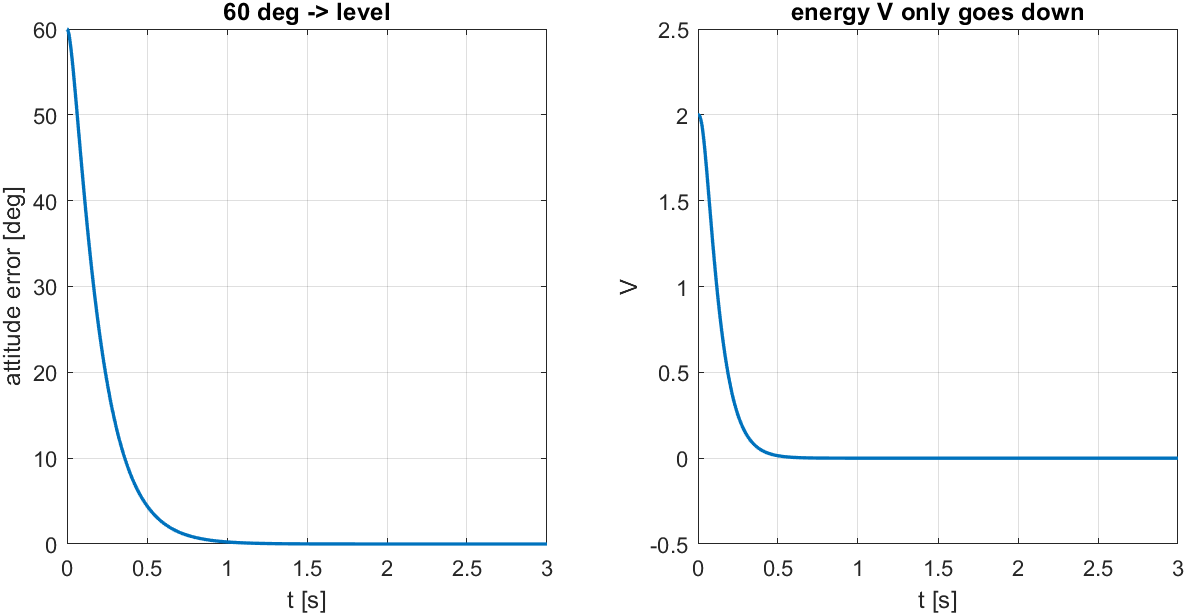
\includegraphics[width=0.85\linewidth]{M1_3_SO3_Control_Closed_Loop_1.png}
  \caption{Block 7 alone: from 60$^\circ$ to level. Right: the energy $V$ only goes down, as the proof promised.}
  \label{fig:att}
\end{figure}

\begin{toycode}{M1\_3\_SO3\_Control\_Closed\_Loop}{Block 7}
e_R = 0.5*DroneLib.vee(Rd'*R_hat - R_hat'*Rd)
e_w = w_hat - R_hat'*Rd*w_d
tau = -P.KR*e_R - P.Kw*e_w + cross(w_hat, P.J*w_hat) ...
      - P.J*(DroneLib.hat(w_hat)*R_hat'*Rd*w_d - R_hat'*Rd*wdot_d)
T = dot(Fd, R_hat*P.e3)
\end{toycode}

\begin{real}
Equations (20), (21) and (22) are three functions of our controller, written exactly as above:
\pyfile{134}{142}{\so}{drones\_controller/so3\_controller.py --- equation (20)}
\pyfile{152}{158}{\so}{drones\_controller/so3\_controller.py --- equation (21)}
\pyfile{181}{210}{\so}{drones\_controller/so3\_controller.py --- equation (22)}
Equation (23) is not in the Python code, because our node does not send thrust to ArduPilot (see
\cref{sec:realctrl}). The toy model computes it.
\end{real}

% ---------------------------------------------------------------------
\subsection{Block 8 --- Four motor speeds (control allocation)}
\label{sec:m1b8}
% ---------------------------------------------------------------------

\begin{idea}
The drone does not have a ``torque knob''. It has four motors. Spinning the right-side motors faster rolls it left;
spinning the front ones faster pitches it back; spinning the clockwise pair faster yaws it. Block 8 solves the
reverse problem: which four rotor thrusts give exactly the wanted $T$ and $\vtau$?
\end{idea}

\begin{eqbox}{Equations (24)--(25): control allocation and motor speeds}
\begin{align}
  \begin{bmatrix}T\\ \vtau\end{bmatrix}&=\Gamma\,\vf,\qquad
  \Gamma=\begin{bmatrix}1&1&1&1\\ y_1&y_2&y_3&y_4\\ -x_1&-x_2&-x_3&-x_4\\ \kappa_1c_m&\kappa_2c_m&\kappa_3c_m&\kappa_4c_m\end{bmatrix} \tag{24}\label{eq:24}\\
  \Omega_i&=\sqrt{\frac{\big(\Gamma^{-1}\vu\big)_i}{k_f}}\quad\text{clipped to }[\Omega_{\min},\Omega_{\max}] \tag{25}\label{eq:25}
\end{align}
$f_i$: thrust of rotor $i$; $(x_i,y_i)$: its position on the frame; $\kappa_i=\pm1$: its spin direction; $c_m$: yaw torque per newton;
$k_f$: thrust constant ($f_i=k_f\Omega_i^2$).
\end{eqbox}

\subsubsection*{Derivation}
Each rotor $i$ pushes up with $f_i$ at the point $\bm r_i=[x_i,y_i,0]$ of the frame.
\begin{itemize}
  \item Total thrust: the pushes add up, $T=f_1+f_2+f_3+f_4$ (row 1 of $\Gamma$).
  \item Roll and pitch torque: a force at a distance creates a torque $\bm r_i\times f_i\ve_3=f_i[y_i,\,-x_i,\,0]$
        (rows 2 and 3). A rotor on the right ($y_i<0$) creates negative roll torque.
  \item Yaw torque: air resists each spinning propeller, so each motor twists the body the opposite way with a torque
        proportional to its thrust, $\kappa_ic_mf_i$ (row 4).
\end{itemize}
A propeller's thrust grows with the square of its speed: $f_i=k_f\Omega_i^2$. Inverting both relations gives (25).
Motors cannot spin backwards or faster than their maximum, so the speeds are clipped.

For the Iris (ArduPilot ``Quad-X'': 1 front-right CCW, 2 back-left CCW, 3 front-left CW, 4 back-right CW):
\[
\Gamma=\begin{bmatrix}1&1&1&1\\-0.22&0.22&0.22&-0.22\\-0.13&0.13&-0.13&0.13\\-0.016&-0.016&0.016&0.016\end{bmatrix}.
\]

\begin{toy}[hover, and the roll correction of block 7]
\textbf{Hover} $\vu=[14.715,0,0,0]$: by symmetry every rotor gives $f_i=14.715/4=3.679$\,N, so
$\Omega_i=\sqrt{3.679/8.549\times10^{-6}}=656$\,rad/s (about 6260\,rpm).

\textbf{Roll correction} $\vu=[14.491,\,-0.8546,\,0,\,0]$: by symmetry $f_1=f_4=a$ and $f_2=f_3=b$. Row 1:
$2a+2b=14.491$. Row 2: $-0.22a+0.22b+0.22b-0.22a=0.44(b-a)=-0.8546$. Solving: $a=4.594$\,N, $b=2.652$\,N, so
$\vOmega=[733,\ 557,\ 557,\ 733]$\,rad/s. The right-side rotors (1 and 4) speed up, the left ones slow down, and the
drone rolls back to level.
\end{toy}

\begin{toycode}{M1\_3\_SO3\_Control\_Closed\_Loop}{Block 8 (DroneLib.mixer)}
fr = P.Gamma \ u;                                          % rotor thrusts
fr = min(max(fr, P.kf*P.Omega_min^2), P.kf*P.Omega_max^2); % motor limits
Omega = sqrt(fr/P.kf);                                     % motor speeds
\end{toycode}

\begin{real}
This block lives inside ArduPilot (its ``motor mixer''); our node never talks to the motors directly. The matrix
$\Gamma$ above is the one ArduPilot uses for a Quad-X frame, scaled by the Iris arm lengths.
\end{real}

% ---------------------------------------------------------------------
\subsection{All of Model 1 together: the closed loop}
\label{sec:m1loop}
% ---------------------------------------------------------------------

The last section of \code{M1\_3} connects everything as in \cref{fig:loop}: the true drone (block 1) $\rightarrow$
noisy gyro and camera $\rightarrow$ EKF (block 4) $\rightarrow$ controller on the \emph{estimate} (blocks 5--7)
$\rightarrow$ mixer (block 8) $\rightarrow$ the true drone, in gusty wind, following a climbing helix for 25\,s.
After the start-up transient the drone follows the helix with an RMS error of \textbf{4.7\,cm}, the estimator is
accurate to \textbf{2.2\,cm}, and the motors stay between 649 and 664\,rad/s.

\begin{figure}[H]
  \centering
  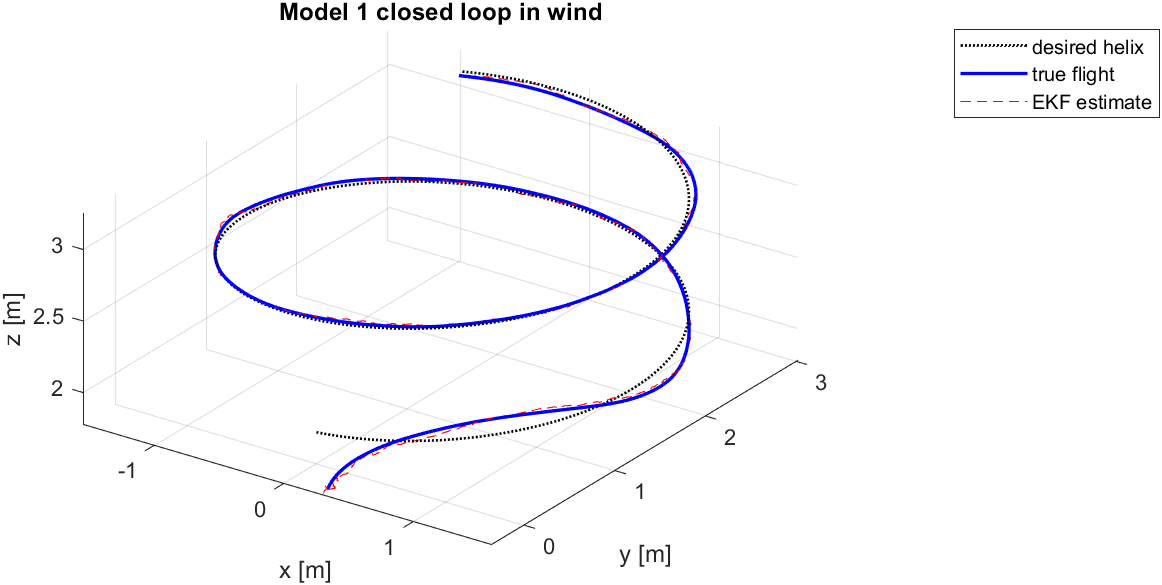
\includegraphics[width=0.6\linewidth]{M1_3_SO3_Control_Closed_Loop_2.png}
  \caption{The complete Model 1 loop in wind: desired helix (dotted), true flight (blue), EKF estimate (red, dashed).}
\end{figure}

\begin{toycode}{M1\_3\_SO3\_Control\_Closed\_Loop}{The closed loop}
ref = DroneLib.helix(t(k));                                   % mission
[ph, vh, Rh, wh] = DroneLib.unpack(xh);                       % the ESTIMATE
u = DroneLib.so3_control(ph, vh, Rh, wh, ref, P);             % blocks 5-7
[Om(:,k), ~, u_app] = DroneLib.mixer(u, P);                   % block 8
x  = DroneLib.rk4(x, u_app, dt, P, gust);                     % block 1, the real drone
[xh, Pk] = DroneLib.ekf_predict(xh, Pk, u_app, dt, P, Q);     % block 4
\end{toycode}

\subsection*{Recap of Model 1}
\begin{center}\small
\begin{tabularx}{\linewidth}{@{}c >{\raggedright\arraybackslash}p{2.8cm} >{\raggedright\arraybackslash}p{2.9cm} >{\raggedright\arraybackslash}p{2.4cm} X@{}}
\toprule
\textbf{\#} & \textbf{Block} & \textbf{In} & \textbf{Out} & \textbf{The idea in one sentence}\\
\midrule
1 & Dynamics & thrust, torque & motion & Push along the body's up-axis, gravity pulls down, torque spins the body.\\
2 & Linearization & operating point & $A$, $B$ & Zoomed in, the drone behaves like a linear system.\\
3 & Error dynamics & $A$, $B$, $\Delta t$ & $F$ & Small errors grow linearly, and fast ($t^3$), without feedback.\\
4 & EKF (VIO) & commands, sensors & $\hx_k$, $P_k$ & Predict with physics, correct with camera and IMU, weighted by trust.\\
5 & Position control & $\hp,\hv$, target & $\va_d$ & Pull towards the target like a spring with a damper.\\
6 & Force \& attitude & $\va_d$, yaw & $\vF_d$, $R_d$ & To accelerate sideways, lean; thrust direction = force direction.\\
7 & SO(3) attitude & $\hR,\hw,R_d,\vF_d$ & $\vtau$, $T$ & Twist downhill on the attitude error; the energy always decreases.\\
8 & Allocation & $T$, $\vtau$ & $\Omega_1..\Omega_4$ & Share thrust and torque among four rotors; speed $\propto\sqrt{\text{thrust}}$.\\
\bottomrule
\end{tabularx}
\end{center}

% =====================================================================
\section{How Our ROS~2 Node Actually Controls the Drone}
\label{sec:realctrl}
% =====================================================================

\Cref{sec:model1} explained each equation. This section follows our real program, \code{drones\_controller},
from start-up through one complete control step, line by line, with numbers. At the end you should be able to point
at any line of \code{controller\_node.py} or \code{so3\_controller.py} and say which equation it is and why it is there.

\subsection{Start-up: reading the parameters and building the controller}

When the node starts, it declares every parameter with a default value. ROS~2 then replaces the defaults with the
values in \code{controller.yaml}. For example:
\pyfile{94}{122}{\node}{controller\_node.py --- some of the parameter declarations}
Then it creates the two objects that do the work: the \emph{trajectory generator} (where should I be?) and the
\emph{SO(3) controller} (how do I get there?). The gains are turned into diagonal matrices $K_p,K_v,K_R,K_\omega$ and the
inertia into $J$:
\pyfile{242}{255}{\node}{controller\_node.py --- the two working objects}
\pyfile{19}{30}{\so}{so3\_controller.py --- \_\_init\_\_(): gains become diagonal matrices}
Next it subscribes to the estimator's output and starts a timer that calls \code{control\_loop()} at
\code{control\_rate} = 25 times per second (one call every 40\,ms):
\pyfile{261}{273}{\node}{controller\_node.py --- subscribing to the state estimate}
\pyfile{338}{343}{\node}{controller\_node.py --- the control timer}

\begin{warn}[Small inconsistency to know about]
The default \code{control\_rate} in the code is 50\,Hz, but \code{controller.yaml} sets 25\,Hz. When the node is launched
with the YAML file the rate is 25\,Hz. If it is started without the YAML, it runs at 50\,Hz. The YAML value is the one
we use everywhere in this document.
\end{warn}

\subsection{Between control steps: receiving the state (block 4's output)}

Whenever ArduPilot publishes a new estimate, a \emph{callback} stores it. \code{pose\_callback} stores $\vp$ and turns the
quaternion into $R$ (shown in \cref{sec:m1b1}). \code{twist\_callback} stores $\vv$ and $\vw$:
\pyfile{419}{433}{\node}{controller\_node.py --- twist\_callback()}
Both remember \emph{when} the data arrived, so that the control step can refuse to use old data.

\subsection{One control step, line by line}

Every 40\,ms the timer calls \code{control\_loop()}:
\pyfile{526}{543}{\node}{controller\_node.py --- control\_loop(), first part}
\begin{enumerate}
  \item \code{state\_is\_valid()}: is every part of the state present, younger than 0.5\,s and a finite number? If not,
        \emph{do nothing} this step (safety).
  \item \code{get\_desired\_state()}: the mission. Today it is a fixed waypoint, so $\vp_d=[0,0,2]$, $\vv_d=\va_d=\bm0$,
        $\psi_d=0$, $\vw_d=\dot\vw_d=\bm0$:
        \pyfile{11}{29}{\traj}{trajectory\_generator.py --- get\_desired\_state()}
  \item \code{controller.compute()}: blocks 5, 6 and 7, in that order:
        \pyfile{221}{258}{\so}{so3\_controller.py --- compute(): blocks 5 $\rightarrow$ 6 $\rightarrow$ 7}
  \item Publish every intermediate result on \code{/drones\_controller/...}, so we can plot them while flying.
  \item If \code{enable\_command} is true, send a velocity command (next subsection).
\end{enumerate}

\begin{toy}[one complete control step of our node, with real numbers]
The estimate says the drone is at $\vp=[0.1,\,-0.2,\,1.5]$\,m, climbing at $\vv=[0,0,0.3]$\,m/s, level ($R=I$) and not
turning ($\vw=\bm0$). The waypoint is $[0,0,2]$. Running the real \code{SO3Controller.compute()} on these numbers gives:
\begin{center}\small
\begin{tabular}{@{}l l l l@{}}
\toprule
\textbf{Output} & \textbf{Equation} & \textbf{Value} & \textbf{Meaning}\\
\midrule
\code{e\_p} & (15) & $[-0.1,\ 0.2,\ 0.5]$\,m & target is 10\,cm west, 20\,cm north, 50\,cm up\\
\code{e\_v} & (15) & $[0,\ 0,\ -0.3]$\,m/s & already climbing a bit\\
\code{F\_d} & (16)--(17) & $[-0.225,\ 0.450,\ 15.540]$\,N & push mostly up, slightly towards the target\\
\code{R\_d} & (18)--(19) & tilt of 1.85$^\circ$ & lean slightly towards $-x$, $+y$\\
\code{e\_R} & (20) & $[0.0289,\ 0.0145,\ -0.0002]$ & the drone is level but should lean\\
\code{e\_omega} & (21) & $[0,\ 0,\ 0]$ & no spin, none wanted\\
\code{M\_d} & (22) & $[-0.1158,\ -0.0579,\ 0.0004]$\,N\,m & twist towards the lean\\
\bottomrule
\end{tabular}
\end{center}
Check the torque: $-K_R\ve_R=-[4(0.0289),\ 4(0.0145),\ 2(-0.0002)]=[-0.1158,\ -0.0579,\ 0.0004]$, and $\ve_\omega=0$ adds
nothing. A torque about $-x$ tips the top of the drone towards $+y$, and a torque about $-y$ tips it towards $-x$: exactly the
direction of $\vF_d$. Every number agrees with the toy model (\cref{sec:m1b5,sec:m1b6,sec:m1b7}).
\end{toy}

\subsection{What is actually sent to the drone: the velocity command}

ArduPilot's ROS~2 interface \code{/ap/v1/cmd\_vel} accepts a \emph{velocity}, not a force and torque. So our node does
not send $\vF_d$ or $\vtau$ (they are published only for monitoring). Instead \code{publish\_velocity\_command()} turns
the position and velocity errors into a velocity request:
\pyfile{670}{696}{\node}{controller\_node.py --- publish\_velocity\_command(): the velocity law}
\[
\vv_{\text{cmd}}=0.8\,\ve_p+0.2\,\ve_v,\qquad\text{and if }\|\vv_{\text{cmd}}\|>1\text{ m/s, scale it down to length 1 m/s}.
\]
This is again a spring (0.8: ``go towards the target, faster when further away'') and a damper (0.2: ``slow down if you are
already moving''). The scaling keeps the \emph{direction} and enforces \code{max\_velocity}.

\begin{toy}[the velocity command]
\textbf{Close to the target} (same state as above): $\vv_{\text{cmd}}=0.8[-0.1,0.2,0.5]+0.2[0,0,-0.3]=[-0.08,\ 0.16,\ 0.34]$\,m/s,
length 0.38\,m/s, below the limit, sent as it is.

\textbf{Far from the target}: drone at $[3,\,-2,\,0.5]$, at rest. $\ve_p=[-3,\,2,\,1.5]$, so
$\vv_{\text{cmd}}=[-2.4,\ 1.6,\ 1.2]$, length 3.12\,m/s, too fast. Scaled by $1/3.12$: $[-0.768,\ 0.512,\ 0.384]$\,m/s,
length exactly 1\,m/s, still pointing straight at the target.
\end{toy}

ArduPilot then does the rest. Inside the flight controller it runs its own version of blocks 5--8: a velocity controller
that asks for an acceleration, which becomes a lean angle, which an attitude controller turns into torques, which the
mixer turns into motor speeds. So the whole chain of \cref{sec:model1} still happens; our node does the outer
``where should I go'' part and ArduPilot the inner, fast part.

\begin{warn}[Two things to check in the simulator]
\begin{itemize}
  \item \textbf{The sign of $z$.} The last lines send \code{linear.z = -velocity\_command[2]}:
        \pyfile{709}{719}{\node}{controller\_node.py --- filling the message}
        The pose and twist that we read are in ENU ($z$ up), and the header says \code{"map"}. If ArduPilot reads this
        command in ENU too, the minus sign makes the drone go \emph{down} when it should go up. It is only right if the
        interface expects $z$ pointing down (NED). This must be checked once in SITL: command a small climb and watch
        the altitude.
  \item \textbf{Safety switch.} \code{enable\_command} is \code{false} in the YAML, so by default the node only computes and
        publishes; nothing moves until we deliberately switch it on.
\end{itemize}
\end{warn}

\subsection{Summary: from equation to line of code}

\begin{center}\small
\begin{tabularx}{\linewidth}{@{}l l X@{}}
\toprule
\textbf{Equation} & \textbf{Block} & \textbf{Where in our code}\\
\midrule
(1)--(4) & dynamics & Gazebo (not in our code); result read in \code{pose\_callback}, \code{twist\_callback}\\
$R$ from quaternion & -- & \code{state\_adapter.py}: \code{quaternion\_to\_rotation\_matrix()}, lines 4--42\\
(5)--(14) & EKF (VIO) & ArduPilot EKF3; freshness check in \code{state\_is\_valid()}, lines 447--496\\
(15) & position errors & \code{so3\_controller.py}: \code{compute\_position\_errors()}, lines 32--40\\
(16)--(17) & desired force & \code{so3\_controller.py}: \code{compute\_desired\_force()}, lines 42--74\\
(18)--(19) & desired attitude & \code{so3\_controller.py}: \code{compute\_desired\_attitude()}, lines 76--126\\
(20) & attitude error & \code{so3\_controller.py}: \code{compute\_attitude\_error()}, lines 128--142\\
(21) & rate error & \code{so3\_controller.py}: \code{compute\_angular\_velocity\_error()}, lines 144--158\\
(22) & torque & \code{so3\_controller.py}: \code{compute\_moment()}, lines 160--210\\
(23)--(25) & thrust, mixer & ArduPilot (our node sends a velocity instead)\\
$\vv_{\text{cmd}}$ & command & \code{controller\_node.py}: \code{publish\_velocity\_command()}, lines 644--734\\
\bottomrule
\end{tabularx}
\end{center}

% =====================================================================
\section{Model 2: Learning from Data and Optimal Control}
\label{sec:model2}
% =====================================================================

Model~1 needs the physics: the mass $m$, the inertia $J$, the rotor constants. Model~2 asks a different question:
\emph{if we only had recorded flight data, could we still build a good controller?} It learns a linear model from data
(blocks 1--2) and then computes the best controller for that model in two ways (\cref{fig:flow2}):
\begin{itemize}
  \item \textbf{LQR} (blocks 3--6): the mathematically best \emph{linear} controller. Very cheap to run, but it knows
        nothing about limits.
  \item \textbf{MPC} (blocks 7--9): plans the next second optimally \emph{and} respects limits such as
        ``never faster than 1\,m/s'', at the cost of solving a small optimisation problem every step.
\end{itemize}
Block 10 flies the real, nonlinear drone with the result. All Model~2 matrices are in \emph{discrete time} with
$\Delta t=0.04$\,s (25\,Hz, the \code{control\_rate}): $\vx_{k+1}=A\vx_k+B\vu_k$.
Toy model files:
\begin{itemize}
  \item \code{M2\_1\_Flight\_Data\_DMDc.mlx} (blocks 1--2),
  \item \code{M2\_2\_LQR\_Bellman\_Riccati\_DARE.mlx} (blocks 3--6),
  \item \code{M2\_3\_MPC\_QP\_Apply\_to\_Drone.mlx} (blocks 7--10).
\end{itemize}

% ---------------------------------------------------------------------
\subsection{Block 1 --- Recording flight data}
\label{sec:m2b1}
% ---------------------------------------------------------------------

\begin{idea}
Fly the drone and write down, 25 times per second, where it was and what we told it to do. To make the data useful we
measure everything as a \emph{difference from hover}, and we deliberately give the drone small random pushes so that the
data contains enough variety to learn from.
\end{idea}

\begin{eqbox}{Equation (M2.1): sampled state and input, as deviations from hover}
\begin{equation}
  \vx_k=\begin{bmatrix}\vp(t_k)-\vp_{\mathrm{ref}}\\ \vv(t_k)\\ \Log\big(R(t_k)\big)\\ \vw(t_k)\end{bmatrix}\in\R^{12},\qquad
  \vu_k=\begin{bmatrix}T(t_k)-mg_0\\ \vtau(t_k)\end{bmatrix}\in\R^{4},\qquad t_k=k\,\Delta t . \tag{M2.1}
\end{equation}
\end{eqbox}

\subsubsection*{Why it is written this way}
\textbf{Differences from hover.} Hover is a balance point of (1)--(4): level, still, thrust $=$ weight, every rate is
zero. Near it, the linear model $\vx_{k+1}=A\vx_k+B\vu_k$ has \emph{no constant term}. If we used the raw thrust $T$
instead of $T-mg_0$, gravity would appear as a constant $+mg_0$ that this form cannot represent, and the fit would be poor.

\textbf{Attitude as three numbers.} The learning method needs plain vectors, so the rotation matrix is replaced by its
rotation vector $\Log(R)$ (\cref{sec:maths}). Near hover these three numbers are roll, pitch and yaw in radians.

\textbf{A pilot plus random pushes.} A free drone is unstable (\cref{sec:m1b3}), so the data must be recorded with some
stabilising pilot flying it (the role ArduPilot plays). But if the input were \emph{only} feedback, $\vu=-K_0\vx$, every
input would be a fixed combination of the states, and the computer could not tell ``what the drone does'' apart from
``what the pilot does''. Adding small random pushes ($\pm2$\,N of thrust, $\pm0.03$\,N\,m of torque, each held for 0.2\,s) fixes
this. This is called \textbf{persistent excitation}.

\begin{toy}[the recorded data set]
Five flights of 25\,s each at 25\,Hz, starting from random points near $[0,0,2]$\,m: $5\times625$ samples of
$\vx_k\in\R^{12}$ and $\vu_k\in\R^4$, with a little sensor noise. Flights 1--4 are used to learn, flight 5 is kept back to
test. The largest tilt in all the data is 6.5$^\circ$, well inside the range where the drone is nearly linear (\cref{sec:m1b2}).
\end{toy}

\begin{figure}[H]
  \centering
  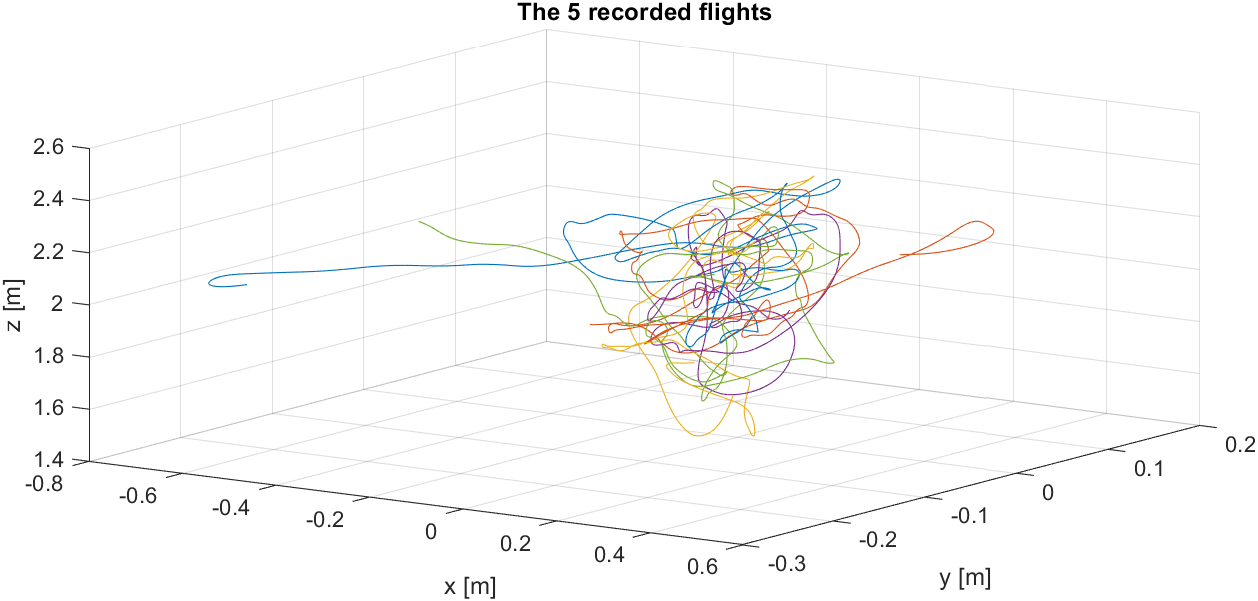
\includegraphics[width=0.55\linewidth]{M2_1_Flight_Data_DMDc_1.png}
  \caption{The five recorded flights around the hover point.}
\end{figure}

\begin{toycode}{M2\_1\_Flight\_Data\_DMDc}{Block 1}
Xr(:,k) = DroneLib.to_dev(x, P.p_hover) + noise;        % logged state x_k
if mod(k-1, 5) == 0                                       % new random push
    exc = [2; 0.03; 0.03; 0.01].*(2*rand(4,1) - 1);       %   every 0.2 s
end
[~, ~, u_app] = DroneLib.mixer(u_trim + DroneLib.pilot(Xr(:,k), P) + exc, P);
Ur(:,k) = u_app - u_trim;                                % logged input u_k
\end{toycode}

\begin{real}
In the project, block 1 is a ROS~2 bag recording of \code{/ap/v1/pose/filtered}, \code{/ap/v1/twist/filtered} and the
commands we send, from SITL or a real flight (\code{ros2 bag record ...}). The pose and twist are exactly the inputs our
node already reads, so no new sensor is needed, and nothing about mass or inertia needs to be known.
\end{real}

% ---------------------------------------------------------------------
\subsection{Block 2 --- DMDc: learning $A$ and $B$ from the data}
\label{sec:m2b2}
% ---------------------------------------------------------------------

\begin{idea}
Look at thousands of moments of the form ``the drone was \emph{here}, we pushed like \emph{this}, and 40\,ms later it was
\emph{there}'', and find the single linear rule $\vx_{k+1}=A\vx_k+B\vu_k$ that explains all of them best. It is curve
fitting for motion. It is the EDMD idea from the course notes (\code{K = Psi2*pinv(Psi1)}) with the input added; the
name DMDc means \emph{Dynamic Mode Decomposition with control}.
\end{idea}

\begin{eqbox}{Equations (M2.2)--(M2.4): snapshot matrices and the least-squares model}
\begin{align}
  X=\big[\vx_1\ \cdots\ \vx_{N-1}\big],\quad X^+&=\big[\vx_2\ \cdots\ \vx_{N}\big],\quad U=\big[\vu_1\ \cdots\ \vu_{N-1}\big] \tag{M2.2}\\
  \big[\,A\ \ B\,\big]&=X^+\begin{bmatrix}X\\ U\end{bmatrix}^{\dagger} \tag{M2.3}\\
  \vx_{k+1}&\approx A\,\vx_k+B\,\vu_k \tag{M2.4}
\end{align}
\end{eqbox}

\subsubsection*{Derivation}
Put the states side by side in a matrix $X$, the same states shifted one step later in $X^+$, and the inputs in $U$. We want
one matrix $G=[A\ \ B]$ such that, for every column,
\[
\vx_{k+1}=A\vx_k+B\vu_k=G\begin{bmatrix}\vx_k\\ \vu_k\end{bmatrix}.
\]
Written for all columns at once:
\[
X^+\approx G\,\Omega,\qquad \Omega=\begin{bmatrix}X\\U\end{bmatrix}.
\]
With noisy data this cannot hold exactly, so we choose the $G$ with the smallest total squared prediction error
$\|X^+-G\Omega\|^2$ (least squares, \cref{sec:lsq}). Setting the derivative with respect to $G$ to zero:
\[
-2\,(X^+-G\Omega)\,\Omega^\top=0\quad\Longrightarrow\quad G\,\Omega\Omega^\top=X^+\Omega^\top
\quad\Longrightarrow\quad G=X^+\Omega^\top(\Omega\Omega^\top)^{-1}=X^+\Omega^\dagger .
\]
$\Omega\Omega^\top$ is a $16\times16$ matrix. It can only be inverted if $\Omega$ has 16 independent rows ($12+4$), which is
exactly what the random pushes of block 1 guarantee. The first 12 columns of $G$ are $A$ and the last 4 are $B$.

\textbf{What should the answer be?} If the data came from the physics of Model~1, the exact answer is the discrete
version of the Jacobians \eqref{eq:AB}: $A=e^{A_c\Delta t}$ and $B=\int_0^{\Delta t}e^{A_cs}ds\,B_c$ (the ``zero-order hold'':
the input is held constant for one step). So we can check DMDc against the physics.

\begin{toy}[DMDc by hand, one number]
The true system is $x_{k+1}=0.9x_k+0.5u_k$, but we pretend not to know $0.9$ and $0.5$. Three recorded steps:
$X=[1,\ 1.4,\ 0.76]$, $U=[1,\ -1,\ 0.5]$, $X^+=[1.4,\ 0.76,\ 0.934]$. Then
\[
\Omega\Omega^\top=\begin{bmatrix}1+1.96+0.5776 & 1-1.4+0.38\\ 1-1.4+0.38 & 1+1+0.25\end{bmatrix}=\begin{bmatrix}3.5376&-0.02\\-0.02&2.25\end{bmatrix},
\]
\[
X^+\Omega^\top=\begin{bmatrix}1.4+1.064+0.70984 & 1.4-0.76+0.467\end{bmatrix}=\begin{bmatrix}3.17384&1.107\end{bmatrix},
\]
\[
[a\ \ b]=\frac{1}{3.5376\cdot2.25-0.02^2}\begin{bmatrix}3.17384&1.107\end{bmatrix}\begin{bmatrix}2.25&0.02\\0.02&3.5376\end{bmatrix}=\begin{bmatrix}0.9000&0.5000\end{bmatrix}.
\]
The hidden numbers are found exactly, because this data has no noise.

\textbf{The drone} (2500 snapshots, rank of $\Omega$ = 16):
\begin{center}\small
\begin{tabular}{@{}llrr@{}}
\toprule
entry & physical meaning & learned by DMDc & physics\\
\midrule
$A_{1,4}$ & $\Delta t$ (position from velocity) & 0.0399 & 0.0400\\
$A_{4,8}$ & $g_0\Delta t$ ($v_x$ from pitch) & 0.3909 & 0.3924\\
$A_{5,7}$ & $-g_0\Delta t$ ($v_y$ from roll) & $-0.3862$ & $-0.3924$\\
$B_{6,1}$ & $\Delta t/m$ ($v_z$ from thrust) & 0.0268 & 0.0267\\
$B_{10,2}$ & $\Delta t/J_x$ (roll rate from roll torque) & 2.0007 & 2.0000\\
$B_{12,4}$ & $\Delta t/J_z$ (yaw rate from yaw torque) & 1.0096 & 1.0000\\
\bottomrule
\end{tabular}
\end{center}
Overall the learned $A$ is within 2.6\% of the physics and $B$ within 1.1\%. The data even ``knows'' the mass:
$\Delta t/B_{6,1}=1.494$\,kg (true: 1.5\,kg). On flight 5, which was never used for learning, predicting 1\,s ahead from the
inputs alone gives a position error of 1.33\,cm, against 1.26\,cm for the exact physics model.
\end{toy}

\begin{figure}[H]
  \centering
  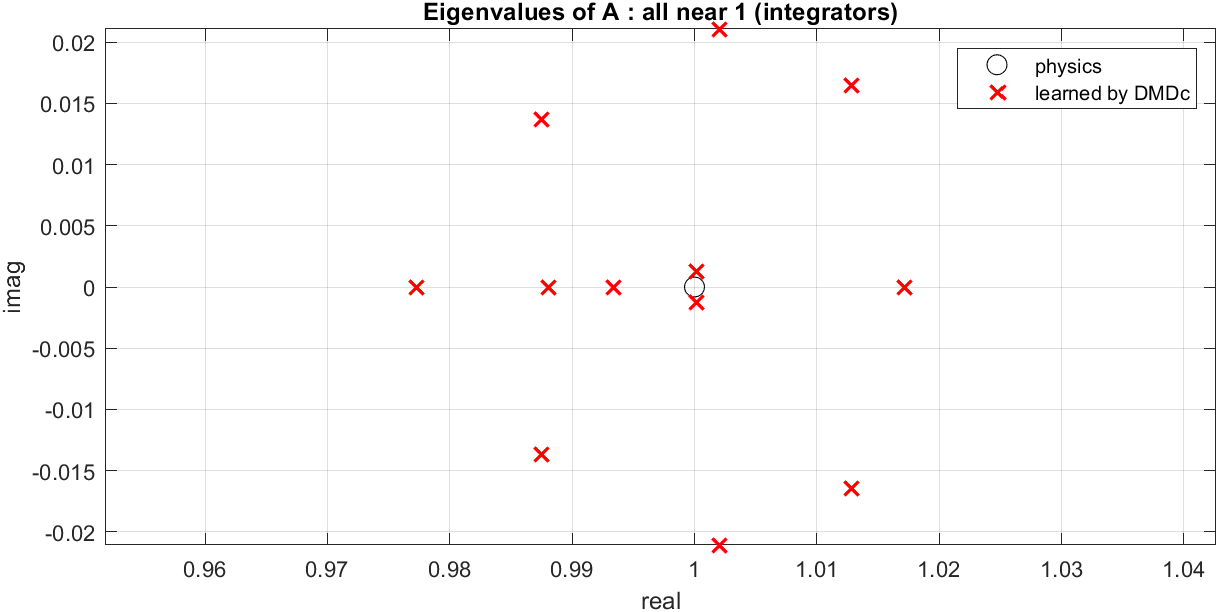
\includegraphics[width=0.5\linewidth]{M2_1_Flight_Data_DMDc_2.png}
  \caption{Eigenvalues of the learned $A$ (crosses) and of the physics (circles). All lie at or very near 1: a
  chain of integrators, exactly as block 3 of Model 1 predicted.}
\end{figure}

\begin{toycode}{M2\_1\_Flight\_Data\_DMDc}{Block 2}
Omega = [Xa; Ua];
rank_Omega = rank(Omega)                % must be 12 + 4 = 16 (enough excitation)
G = Xpa*pinv(Omega);                    % (M2.3)
A = G(:, 1:12);
B = G(:, 13:16);
\end{toycode}

\begin{real}
DMDc runs offline, on a laptop, on a recorded bag. If the drone changes (a heavier camera, a new battery, a different
frame), a two-minute flight is enough to learn the new $A$ and $B$, without measuring anything by hand.
\end{real}

% ---------------------------------------------------------------------
\subsection{Block 3 --- The Bellman equation: what is ``the best'' controller?}
\label{sec:m2b3}
% ---------------------------------------------------------------------

\begin{idea}
Before we can find the best controller we must say what ``best'' means. We give the flight a \emph{score}: every moment we
are off target costs points, and every push of the motors costs points. The best controller is the one with the lowest
total score. Bellman's idea: the best plan from here is the best \emph{first move} plus the best plan from wherever that
move takes us.
\end{idea}

\begin{eqbox}{Equations (M2.5)--(M2.7): cost, Bellman equation, quadratic value function}
\begin{align}
  J&=\sum_{k=0}^{\infty}\big(\vx_k^\top Q\,\vx_k+\vu_k^\top R\,\vu_k\big) \tag{M2.5}\\
  V(\vx_k)&=\min_{\vu_k}\Big[\vx_k^\top Q\vx_k+\vu_k^\top R\vu_k+V(\vx_{k+1})\Big],\qquad \vx_{k+1}=A\vx_k+B\vu_k \tag{M2.6}\\
  V(\vx)&=\vx^\top P\,\vx \tag{M2.7}
\end{align}
\end{eqbox}

\subsubsection*{(M2.5) The score}
$\vx^\top Q\vx$ is a weighted sum of squared errors and $\vu^\top R\vu$ a weighted sum of squared pushes. Big $Q$: ``I hate
being off target''. Big $R$: ``I hate using the motors''. We choose them with \textbf{Bryson's rule}: $Q_{ii}=1/x_{i,\max}^2$
and $R_{jj}=1/u_{j,\max}^2$, where $x_{i,\max}$ is the largest error we are willing to accept:
\begin{center}\small
\begin{tabular}{@{}lll@{}}
\toprule
quantity & largest acceptable value & weight\\
\midrule
position error & 0.5\,m & $1/0.5^2=4$\\
velocity & 1\,m/s (\code{max\_velocity}) & 1\\
roll, pitch / yaw & 0.2\,rad / 0.5\,rad & 25 / 4\\
angular rates & 1\,rad/s & 1\\
extra thrust & 5\,N & 0.04\\
roll, pitch torque / yaw torque & 0.2\,N\,m / 0.05\,N\,m & 25 / 400\\
\bottomrule
\end{tabular}
\end{center}
So a 50\,cm position error ``hurts'' as much as flying at 1\,m/s, tilting 0.2\,rad, or using 5\,N of extra thrust.

\subsubsection*{(M2.6) Principle of optimality}
Split the infinite sum into the first step and all the rest:
\[
V(\vx_k)=\min_{\vu_k,\vu_{k+1},\dots}\Big[\ell(\vx_k,\vu_k)+\sum_{j>k}\ell(\vx_j,\vu_j)\Big]
=\min_{\vu_k}\Big[\ell(\vx_k,\vu_k)+\underbrace{\min_{\vu_{k+1},\dots}\sum_{j>k}\ell(\vx_j,\vu_j)}_{V(\vx_{k+1})}\Big],
\]
where $\ell$ is the score of one step. Whatever the first move is, the remaining moves must be the best ones for the place
it leads to; otherwise we could improve them and lower the total. A problem with infinitely many unknowns becomes a
problem with \emph{one} unknown, $\vu_k$.

\subsubsection*{(M2.7) The value function is a bowl}
Guess that the lowest possible score from $\vx$ is a quadratic, $V(\vx)=\vx^\top P\vx$. Then the bracket in (M2.6) is a
quadratic in $\vu_k$. Its minimum (block 4) is linear in $\vx_k$, and putting it back gives again a quadratic in $\vx_k$
(block 5). The guess is self-consistent, so all that is left to find is the matrix $P$.

\begin{toy}[one Bellman step by hand]
System $x_{k+1}=1.1x_k+0.5u_k$ (on its own it grows 10\% per step: unstable). $q=r=1$, the next value is $V(x)=x^2$, and
we are at $x=1$:
\[
\text{score}(u)=\underbrace{1}_{qx^2}+\underbrace{u^2}_{ru^2}+\underbrace{(1.1+0.5u)^2}_{V(x_{k+1})},\qquad
\frac{d}{du}=2u+(1.1+0.5u)=0\ \Rightarrow\ u^*=-\frac{1.1}{2.5}=-0.44,
\]
\[
V(1)=1+0.1936+(1.1-0.22)^2=1.968 .
\]
MATLAB's \code{fminsearch} on the same function returns $u^*=-0.4400$ and $1.9680$.
\end{toy}

\begin{toycode}{M2\_2\_LQR\_Bellman\_Riccati\_DARE}{Block 3}
a = 1.1;  b = 0.5;  q = 1;  r = 1;
cost = @(u) q*1^2 + r*u.^2 + 1*(a*1 + b*u).^2;
u_star = -a*b/(r + b^2)                 % by hand
[u_search, V1] = fminsearch(cost, 0)   % by the inbuilt optimiser
\end{toycode}

% ---------------------------------------------------------------------
\subsection{Block 4 --- The Linear Quadratic Regulator (LQR)}
\label{sec:m2b4}
% ---------------------------------------------------------------------

\begin{idea}
Do the minimisation of block 3 once, in general, with matrices. The answer is beautifully simple: the best push is a fixed
matrix $K$ times the current error. The whole controller is one $4\times12$ table of numbers.
\end{idea}

\begin{eqbox}{Equations (M2.8)--(M2.9): optimal gain and control law}
\begin{align}
  K&=\big(R+B^\top PB\big)^{-1}B^\top PA \tag{M2.8}\\
  \vu_k&=-K\,\vx_k \tag{M2.9}
\end{align}
\end{eqbox}

\subsubsection*{Derivation}
Put $V(\vx_{k+1})=(A\vx+B\vu)^\top P(A\vx+B\vu)$ into the bracket of (M2.6). It is a bowl in $\vu$ (\cref{sec:minquad}).
Its slope with respect to $\vu$, using $\partial(\vu^\top M\vu)/\partial\vu=2M\vu$, must be zero:
\[
2R\vu+2B^\top P(A\vx+B\vu)=\bm0\quad\Longrightarrow\quad(R+B^\top PB)\,\vu=-B^\top PA\,\vx .
\]
$R+B^\top PB$ is positive definite (because $R$ is), so it can be inverted and the point really is the bottom of the bowl.
Hence $\vu^*=-(R+B^\top PB)^{-1}B^\top PA\,\vx=-K\vx$.

\begin{toy}[the scalar system, and the drone's gain]
With the final $P=3.1215$ (from block 6): $K=\dfrac{ab\,P}{r+b^2P}=\dfrac{1.1\cdot0.5\cdot3.1215}{1+0.25\cdot3.1215}=0.9643$.
With control, $x_{k+1}=(a-bK)x_k=0.6179\,x_k$. Without control the state grew 10\% per step; with LQR it
\emph{shrinks} 38\% per step (\cref{sec:eig}).

\textbf{The drone's $K$}, two of its 48 numbers (from block 6):
\[
\delta T=-9.04\,\delta z-6.92\,v_z,\qquad
\tau_x=0.273\,\delta y+0.321\,v_y-1.444\,\theta_x-0.276\,\omega_x .
\]
Read them: too high or rising $\Rightarrow$ less thrust. Too far north ($\delta y>0$) $\Rightarrow$ positive roll torque, which
tips the drone towards $-y$, back to the target; but less so if it is already rolled ($\theta_x$) or rolling ($\omega_x$).
\end{toy}

% ---------------------------------------------------------------------
\subsection{Block 5 --- The Riccati recursion: finding $P$ step by step}
\label{sec:m2b5}
% ---------------------------------------------------------------------

\begin{idea}
$K$ needs $P$, and $P$ is ``the lowest score from here''. Start with a controller that looks 0 steps ahead, then 1 step,
then 2, and so on. Each time, the plan sees one more step of the future. After enough steps, looking further does not
change anything: we have the infinite-horizon $P$.
\end{idea}

\begin{eqbox}{Equation (M2.10): Riccati difference equation}
\begin{equation}
  P_{k+1}=A^\top P_kA-A^\top P_kB\big(R+B^\top P_kB\big)^{-1}B^\top P_kA+Q,\qquad P_0=Q \tag{M2.10}
\end{equation}
($k$ counts ``steps of look-ahead'', not time.)
\end{eqbox}

\subsubsection*{Derivation}
Put the best push $\vu^*=-K\vx$ back into the bracket of (M2.6):
\[
V_{\text{new}}(\vx)=\vx^\top\big[Q+K^\top RK+(A-BK)^\top P(A-BK)\big]\vx .
\]
Multiply out $(A-BK)^\top P(A-BK)=A^\top PA-A^\top PBK-K^\top B^\top PA+K^\top B^\top PBK$ and add $K^\top RK$. From (M2.8),
$(R+B^\top PB)K=B^\top PA$, so $K^\top(R+B^\top PB)K=K^\top B^\top PA$, and two terms cancel:
\[
V_{\text{new}}=\vx^\top\big[Q+A^\top PA-A^\top PBK\big]\vx=\vx^\top\big[Q+A^\top PA-A^\top PB(R+B^\top PB)^{-1}B^\top PA\big]\vx .
\]
The matrix in brackets is the new $P$: that is (M2.10).

\begin{toy}[the scalar recursion: $a=1.1$, $b=0.5$, $q=r=1$, $P_0=1$]
\[
P_{k+1}=1+1.21P_k-\frac{(0.55P_k)^2}{1+0.25P_k}
\]
\begin{center}\small
\begin{tabular}{l*{10}{c}}
\toprule
$k$ & 0 & 1 & 2 & 3 & 4 & 5 & 6 & 7 & 8 & $\infty$\\
$P_k$ & 1 & 1.968 & 2.596 & 2.905 & 3.036 & 3.089 & 3.109 & 3.117 & 3.120 & 3.1215\\
\bottomrule
\end{tabular}
\end{center}
$P_1=1.968$ is exactly the Bellman step of block 3. For the drone, starting from $P_0=Q$, the change becomes smaller than
$10^{-12}$ after 236 iterations (\cref{fig:riccati}): looking more than about 10\,s ahead changes nothing.
\end{toy}

\begin{figure}[H]
  \centering
  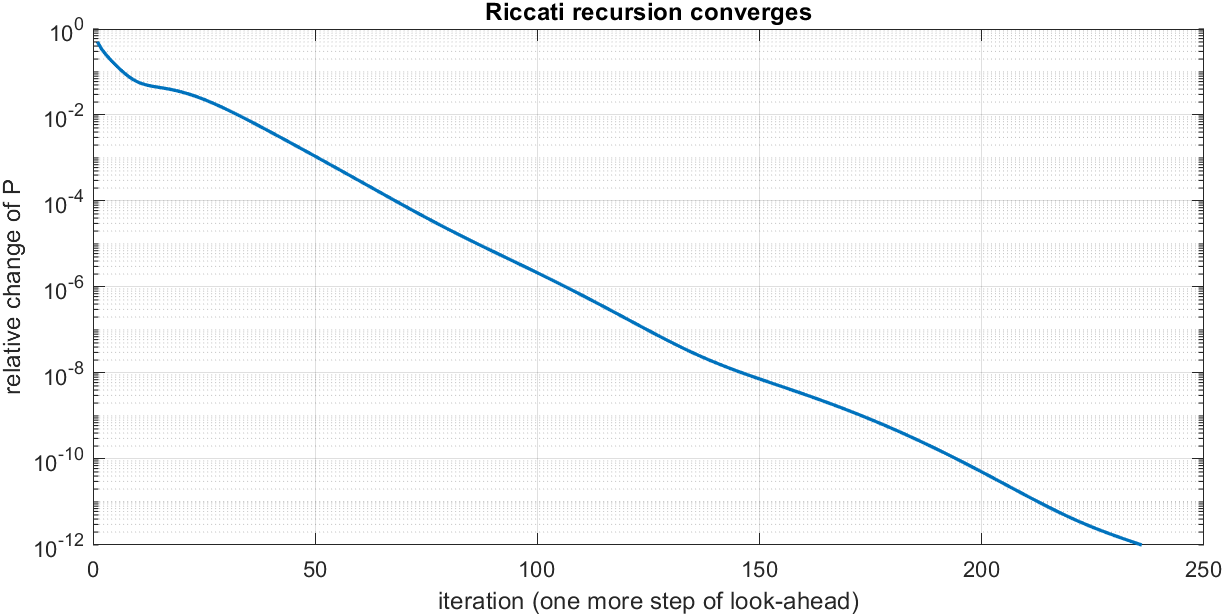
\includegraphics[width=0.55\linewidth]{M2_2_LQR_Bellman_Riccati_DARE_1.png}
  \caption{Riccati recursion for the drone: the change of $P$ falls steadily until it has converged.}
  \label{fig:riccati}
\end{figure}

\begin{toycode}{M2\_2\_LQR\_Bellman\_Riccati\_DARE}{Riccati recursion}
Pk = Q;
for it = 1:5000
    Kk = (R + B'*Pk*B) \ (B'*Pk*A);                       % (M2.8)
    Pn = A'*Pk*A - A'*Pk*B*Kk + Q;                        % (M2.10)
    change(it) = norm(Pn - Pk, 'fro')/norm(Pn, 'fro');
    Pk = Pn;
    if change(it) < 1e-12, break, end
end
\end{toycode}

% ---------------------------------------------------------------------
\subsection{Block 6 --- The DARE: jumping straight to the answer}
\label{sec:m2b6}
% ---------------------------------------------------------------------

\begin{idea}
When the recursion has stopped changing, $P_{k+1}=P_k$. Writing that down gives one equation for the final $P$, the
\emph{Discrete Algebraic Riccati Equation}. It can be solved directly instead of iterating. Its solution gives the final
gain $K$ and also tells us the total score in advance.
\end{idea}

\begin{eqbox}{Equation (M2.11): the Discrete Algebraic Riccati Equation}
\begin{equation}
  P=A^\top PA-A^\top PB\big(R+B^\top PB\big)^{-1}B^\top PA+Q \tag{M2.11}
\end{equation}
\end{eqbox}

\subsubsection*{Two useful facts}
\textbf{The total score is known in advance.} Rearranged, (M2.11) says $P=Q+K^\top RK+(A-BK)^\top P(A-BK)$. Along the
controlled flight $\vx_{k+1}=(A-BK)\vx_k$ this means
$\vx_k^\top P\vx_k-\vx_{k+1}^\top P\vx_{k+1}=\vx_k^\top Q\vx_k+\vu_k^\top R\vu_k$. Adding this up over all steps, everything in
between cancels (like $(a-b)+(b-c)+(c-d)=a-d$) and, because $\vx_k\to0$:
\[
J^*=\vx_0^\top P\,\vx_0 .
\]
\textbf{Solving without a toolbox.} The toy model solves (M2.11) with a standard trick (stable eigenvectors of a
$24\times24$ matrix pencil, \code{DroneLib.dare}), so no Control System Toolbox is needed.

\begin{toy}[the scalar DARE is a quadratic equation]
$P=1+1.21P-\dfrac{0.3025P^2}{1+0.25P}$. Multiply by $(1+0.25P)$ and collect terms: $0.25P^2-0.46P-1=0$, so
\[
P=\frac{0.46+\sqrt{0.46^2+1}}{0.5}=3.1215
\]
(the positive root), exactly the limit of the recursion.

\textbf{The drone.} The DARE solution satisfies (M2.11) to $6.5\times10^{-14}$ and agrees with the 236-step recursion to
$1.6\times10^{-11}$. The learned drone on its own has spectral radius $\rho(A)=1.017>1$ (unstable); with LQR
$\rho(A-BK)=0.950<1$ (stable). Starting 50/30/20\,cm away, the simulated total score is 41.4373, and the prediction
$\vx_0^\top P\vx_0$ is also 41.4373.
\end{toy}

\begin{figure}[H]
  \centering
  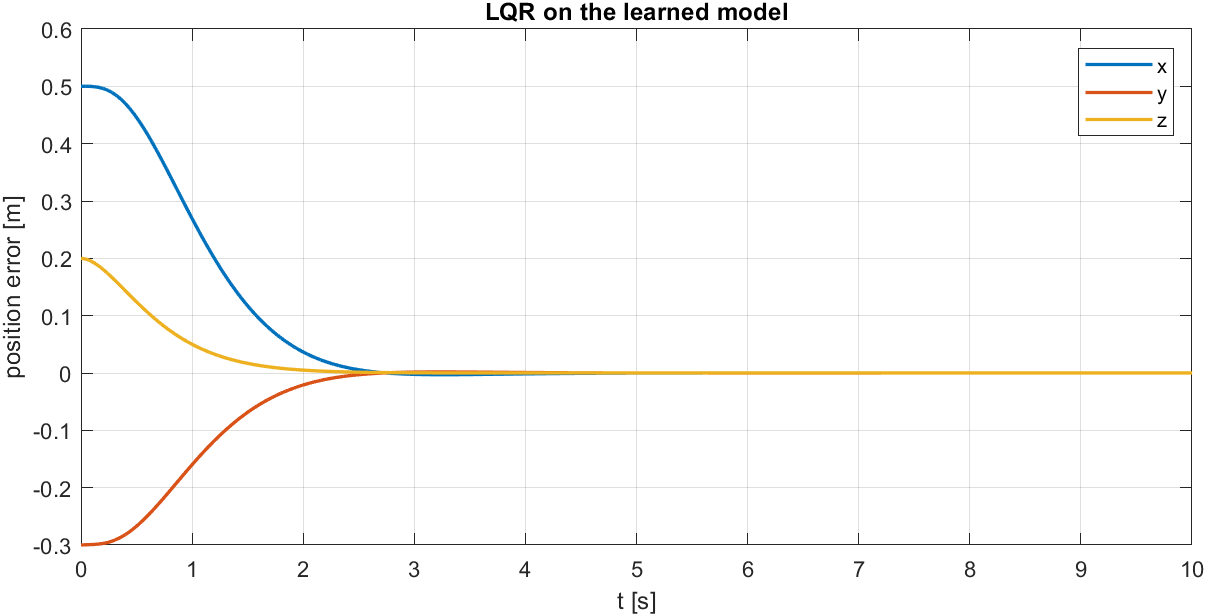
\includegraphics[width=0.55\linewidth]{M2_2_LQR_Bellman_Riccati_DARE_2.png}
  \caption{LQR on the learned model: the position errors die out smoothly.}
\end{figure}

\begin{toycode}{M2\_2\_LQR\_Bellman\_Riccati\_DARE}{DARE solved directly}
P = DroneLib.dare(A, B, Q, R);                     % (M2.11)
K = (R + B'*P*B) \ (B'*P*A);                       % (M2.8)
spectral_radius_closed = max(abs(eig(A - B*K)))   % < 1 : LQR makes it stable
\end{toycode}

\begin{real}[LQR]
On the drone, LQR would be one line every 40\,ms: $\vu=\vu_{\text{trim}}-K\vx$, with $\vx$ from the state estimate. That
costs 48 multiplications, nothing for any flight computer. Its weakness: it knows nothing about limits. Our node's
velocity law $\vv_{\text{cmd}}=0.8\ve_p+0.2\ve_v$ (\cref{sec:realctrl}) is a hand-tuned gain of exactly this kind, and it
needs a separate clip to respect \code{max\_velocity}.
\end{real}

% ---------------------------------------------------------------------
\subsection{Block 7 --- Model Predictive Control (MPC): planning with limits}
\label{sec:m2b7}
% ---------------------------------------------------------------------

\begin{idea}
MPC is like a chess player. Every 40\,ms it imagines the next second of flight, finds the best sequence of moves that never
breaks a rule (``never faster than 1\,m/s'', ``never ask a motor for more than it can give''), plays only the first move,
and then thinks again with the new position.
\end{idea}

\begin{eqbox}{Equation (M2.12): the finite-horizon problem with limits}
\begin{equation}
\begin{aligned}
  \min_{\vu_0,\dots,\vu_{N-1}}\ \ &\sum_{k=0}^{N-1}\big(\vx_k^\top Q\vx_k+\vu_k^\top R\vu_k\big)+\vx_N^\top P_f\,\vx_N\\
  \text{subject to}\ \ &\vx_{k+1}=A\vx_k+B\vu_k,\quad \vx_0=\text{the measured state},\\
  &\vu_{\min}\le\vu_k\le\vu_{\max},\qquad |C\vx_k|\le\vx_{\max}
\end{aligned}\tag{M2.12}
\end{equation}
\end{eqbox}

\subsubsection*{Reasoning}
Real drones have limits: total thrust between about 5 and 25\,N, the torque the rotors can produce, \code{max\_velocity}
= 1\,m/s, and a maximum tilt for a camera. With limits there is no neat formula like LQR's any more, so MPC solves the
problem numerically, and to keep it small:
\begin{itemize}
  \item it only plans $N$ steps ahead ($N=25$: one second);
  \item the infinite rest of the flight is replaced by a final cost $\vx_N^\top P_f\vx_N$.
\end{itemize}
\textbf{Why $P_f=P$ from the DARE.} We showed that $\vx_N^\top P\vx_N$ is \emph{exactly} the best score of the rest of the
flight when no limit is active. So with this choice, when no limit is touched, MPC gives exactly the LQR answer.
That is the link between the two branches of \cref{fig:flow2}.

The drone's limits in the toy model: $5\le T\le25$\,N (so $\delta T\in[-9.715,\,10.285]$\,N), $|\tau_{x,y}|\le0.3$\,N\,m,
$|\tau_z|\le0.05$\,N\,m, $|v_i|\le1$\,m/s, roll and pitch $\le0.35$\,rad (20$^\circ$). $C$ simply picks these five states out of $\vx$.

% ---------------------------------------------------------------------
\subsection{Block 8 --- Turning MPC into a Quadratic Program (QP)}
\label{sec:m2b8}
% ---------------------------------------------------------------------

\begin{idea}
Write every future state in terms of the unknown future pushes. Then the whole problem becomes: ``find the lowest point of
a bowl, but stay inside a fence''. That is called a \emph{quadratic program}, and computers solve it reliably in
milliseconds.
\end{idea}

\begin{eqbox}{Equations (M2.13)--(M2.15): stacked prediction, cost and constraints}
\begin{align}
  \mathbf X=S_x\vx_0+S_u\mathbf U,\qquad
  S_x=\begin{bmatrix}A\\ A^2\\ \vdots\\ A^N\end{bmatrix},\quad
  S_u=\begin{bmatrix}B&0&\cdots&0\\ AB&B&\cdots&0\\ \vdots&&\ddots&\vdots\\ A^{N-1}B&\cdots&AB&B\end{bmatrix} \tag{M2.13}\\[4pt]
  \min_{\mathbf U}\ \tfrac12\mathbf U^\top H\mathbf U+\bm f^\top\mathbf U,\qquad
  H=2\big(S_u^\top\bar QS_u+\bar R\big),\quad \bm f=2S_u^\top\bar QS_x\vx_0 \tag{M2.14}\\[2pt]
  \text{subject to}\quad G\mathbf U\le\bm h,\qquad A_{eq}\mathbf U=\bm b_{eq} \tag{M2.15}
\end{align}
$\mathbf X=[\vx_1;\dots;\vx_N]$, $\mathbf U=[\vu_0;\dots;\vu_{N-1}]$, $\bar Q=\diag(Q,\dots,Q,P_f)$, $\bar R=\diag(R,\dots,R)$.
\end{eqbox}

\subsubsection*{Derivation}
\textbf{(M2.13) Prediction.} Apply the model again and again:
$\vx_1=A\vx_0+B\vu_0$; $\vx_2=A\vx_1+B\vu_1=A^2\vx_0+AB\vu_0+B\vu_1$; and in general
$\vx_k=A^k\vx_0+\sum_{j=0}^{k-1}A^{k-1-j}B\vu_j$. Stacking $k=1..N$ gives (M2.13). The future is \emph{linear} in the unknown
pushes.

\textbf{(M2.14) Cost.} The score is $\vx_0^\top Q\vx_0+\mathbf X^\top\bar Q\mathbf X+\mathbf U^\top\bar R\mathbf U$. Substitute $\mathbf X$
and multiply out:
\[
\mathbf U^\top\big(S_u^\top\bar QS_u+\bar R\big)\mathbf U+2\,\vx_0^\top S_x^\top\bar QS_u\,\mathbf U+\underbrace{\vx_0^\top(Q+S_x^\top\bar QS_x)\vx_0}_{\text{does not depend on }\mathbf U}.
\]
Drop the last part (it does not change where the minimum is) and write the rest as $\tfrac12\mathbf U^\top H\mathbf U+\bm f^\top\mathbf U$.
$H$ is positive definite because $\bar R$ is, so the bowl has \emph{one} bottom and no false minima.

\textbf{(M2.15) Constraints.} Input limits: $\mathbf U\le\mathbf U_{\max}$ and $-\mathbf U\le-\mathbf U_{\min}$. State limits
$|\bar C\mathbf X|\le\bar{\vx}_{\max}$ become, after substituting $\mathbf X$, $\bar CS_u\mathbf U\le\bar{\vx}_{\max}-\bar CS_x\vx_0$ and
$-\bar CS_u\mathbf U\le\bar{\vx}_{\max}+\bar CS_x\vx_0$. Stacked, these give $G\mathbf U\le\bm h$. Equalities $A_{eq}\mathbf U=\bm b_{eq}$
can force, for example, ``be exactly at the target after $N$ steps''.

\textbf{The solver.} The toy model includes its own QP solver (\code{DroneLib.qp}, an interior-point method), so no
Optimization Toolbox is needed. For the drone it needs about 10 iterations.

\begin{toy}[a two-step QP by hand: $a=1.1$, $b=0.5$, $q=r=1$, $N=2$, $P_f=3.1215$, $x_0=1$]
\[
S_x=\begin{bmatrix}1.1\\1.21\end{bmatrix},\quad S_u=\begin{bmatrix}0.5&0\\0.55&0.5\end{bmatrix},\quad
\bar Q=\diag(1,\,3.1215),\quad \bar R=I,
\]
\[
H=\begin{bmatrix}4.3885&1.7168\\1.7168&3.5607\end{bmatrix},\qquad \bm f=\begin{bmatrix}5.2547\\3.7770\end{bmatrix}.
\]
\begin{itemize}
\item \textbf{No limits:} $\mathbf U^*=-H^{-1}\bm f=[-0.9643,\ -0.5958]$. The first move equals the LQR move $-Kx_0=-0.9643$
      \emph{exactly}, as promised by $P_f=P$.
\item \textbf{With $|u_k|\le0.5$:} $\mathbf U^*=[-0.5,\ -0.5]$. Both moves sit on the fence.
\item \textbf{Forcing $x_2=0$} with $[0.55\ \ 0.5]\,\mathbf U=-1.21$: $\mathbf U^*=[-1.3057,\ -0.9837]$. Check:
      $1.21+0.55(-1.3057)+0.5(-0.9837)=0$.
\end{itemize}
\textbf{The drone} ($N=25$): 100 unknowns and 450 inequalities. Starting 5\,cm off, no limit is touched and MPC gives
$[-0.4557,\,-0.0138,\,-0.0137,\,-0.0004]$, the same as $-K\vx_0$ to every printed digit. Starting 2\,m too low, LQR would ask for
$+18.1$\,N of extra thrust, far more than the allowed $+10.285$\,N. MPC uses exactly $+10.285$\,N and plans a climb that
touches, but never exceeds, 1\,m/s.
\end{toy}

\begin{toycode}{M2\_3\_MPC\_QP\_Apply\_to\_Drone}{Block 8, toy example}
Sx = [a; a^2];
Su = [b 0; a*b b];
Qbar = diag([1 Pf]);  Rbar = eye(2);
H = 2*(Su'*Qbar*Su + Rbar)                      % (M2.14)
f = 2*Su'*Qbar*Sx*x0
U_free    = (-H\f)'                             % no limits
U_limited = DroneLib.qp(H, f, [eye(2); -eye(2)], 0.5*ones(4,1))'   % |u| <= 0.5
\end{toycode}

% ---------------------------------------------------------------------
\subsection{Block 9 --- Receding horizon: plan, act a little, plan again}
\label{sec:m2b9}
% ---------------------------------------------------------------------

\begin{eqbox}{Equation (M2.16): receding-horizon control law}
\begin{equation}
  \mathbf U^*(\vx_k)=\big[\vu_0^*,\ \vu_1^*,\ \dots,\ \vu_{N-1}^*\big]
  \quad\Longrightarrow\quad \text{apply only }\vu_0^*,\ \text{measure }\vx_{k+1},\ \text{solve again} \tag{M2.16}
\end{equation}
\end{eqbox}

\begin{idea}
The plan is perfect only for the model, and the model is never perfect (it was learned, and the wind is not in it). So we
never follow a whole plan. We use its first move for 40\,ms, measure where we really are, and plan again. This turns a plan
into feedback: mistakes are corrected 25 times per second instead of piling up.
\end{idea}

\begin{toy}[8 s on the learned model, MPC against LQR]
Start 1.5\,m, 1.0\,m and 1.2\,m away from the target, at rest. MPC never exceeds 1\,m/s (largest speed 1.000\,m/s). LQR,
even when its pushes are clipped to the same motor limits, reaches 1.172\,m/s, because clipping the push does not limit
the \emph{speed}. The median time to solve one QP was 2.6\,ms, well inside the 40\,ms budget.
\end{toy}

\begin{figure}[H]
  \centering
  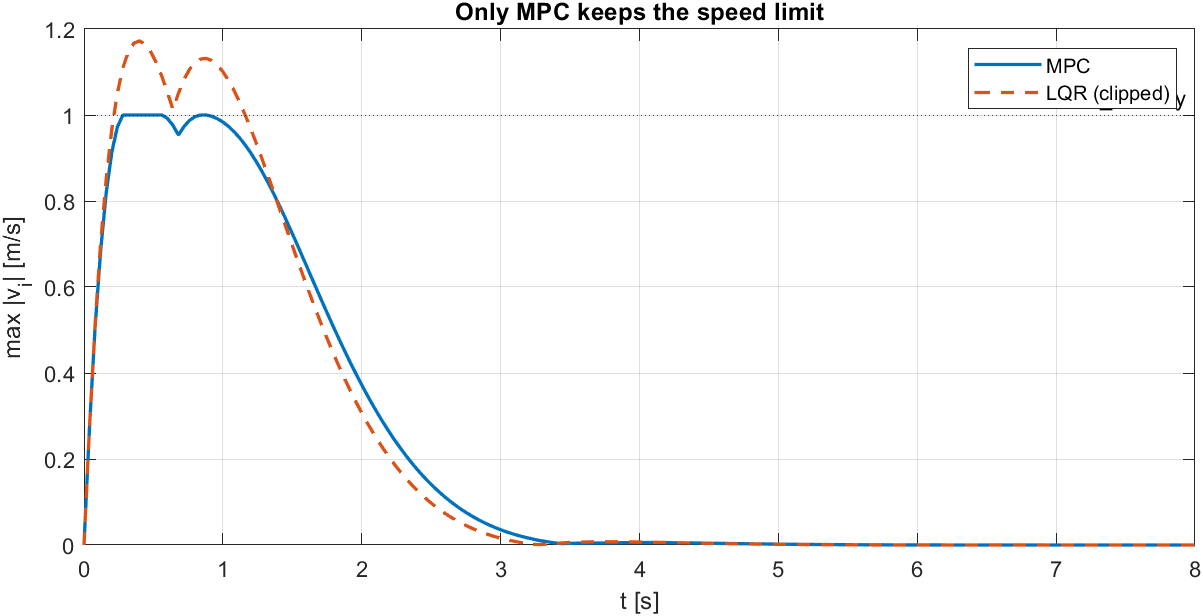
\includegraphics[width=0.6\linewidth]{M2_3_MPC_QP_Apply_to_Drone_1.png}
  \caption{Largest speed component over time: only MPC respects \code{max\_velocity} = 1\,m/s.}
\end{figure}

\begin{toycode}{M2\_3\_MPC\_QP\_Apply\_to\_Drone}{Block 9}
for k = 1:Kn
    um = DroneLib.mpc_solve(mpc, Xm(:,k));            % solve the QP, keep u_0*
    ul = min(max(-K*Xl(:,k), u_min), u_max);          % LQR, clipped
    Xm(:,k+1) = A*Xm(:,k) + B*um;
    Xl(:,k+1) = A*Xl(:,k) + B*ul;
end
\end{toycode}

% ---------------------------------------------------------------------
\needspace{14\baselineskip}
\subsection{Block 10 --- Applying it to the drone}
\label{sec:m2b10}
% ---------------------------------------------------------------------

\begin{eqbox}{Equations (M2.17)--(M2.18): from optimal input to motor speeds}
\begin{align}
  \vu_k&=\vu_{\text{trim}}+\begin{cases}\vu_0^*(\vx_k)&\text{(MPC)}\\ -K\vx_k&\text{(LQR)}\end{cases}
   =\begin{bmatrix}T_k\\ \vtau_k\end{bmatrix},\qquad \vu_{\text{trim}}=\begin{bmatrix}mg_0\\ \bm0\end{bmatrix} \tag{M2.17}\\
  \vf&=\Gamma^{-1}\vu_k,\qquad \Omega_i=\sqrt{f_i/k_f}\qquad(\text{the mixer of block 8 of Model 1}) \tag{M2.18}
\end{align}
\end{eqbox}

\subsubsection*{Reasoning}
The controllers of Model~2 work with \emph{differences from hover}. The motors need real values, so the hover thrust
$mg_0$ is added back. The rest is the same motor mixer as Model~1 (\cref{sec:m1b8}). The loop closes by measuring the new
state of the \emph{real, nonlinear} drone and running block 9 again.

\begin{toy}[one control sample, then a whole flight]
The drone is at $[1.5,\,-1.0,\,0.8]$\,m, at rest; the target is $[0,0,2]$. MPC gives
$\delta\vu=[10.285,\,-0.279,\,-0.300,\,0.002]$: full allowed climb thrust and the largest allowed roll and pitch torques. Adding
hover: $\vu=[25.000,\,-0.279,\,-0.300,\,0.002]$, rotor thrusts $\vf=[7.115,\,5.327,\,6.539,\,6.019]$\,N and motor speeds
$\vOmega=[912,\,789,\,875,\,839]$\,rad/s.

\textbf{The real test}: the nonlinear drone, with gusts and sensor noise, for 10\,s, flown by controllers designed only on
the model learned from data:
\begin{center}\small
\begin{tabular}{lrrr}
\toprule
controller & largest speed [m/s] & error after 10\,s [m] & motor speeds [rad/s]\\
\midrule
MPC & 0.994 & 0.015 & 584 -- 913\\
LQR (clipped) & 1.118 & 0.031 & 613 -- 911\\
\bottomrule
\end{tabular}
\end{center}
Both bring the real drone to the target. Only MPC keeps \code{max\_velocity} = 1\,m/s.
\end{toy}

\begin{figure}[H]
  \centering
  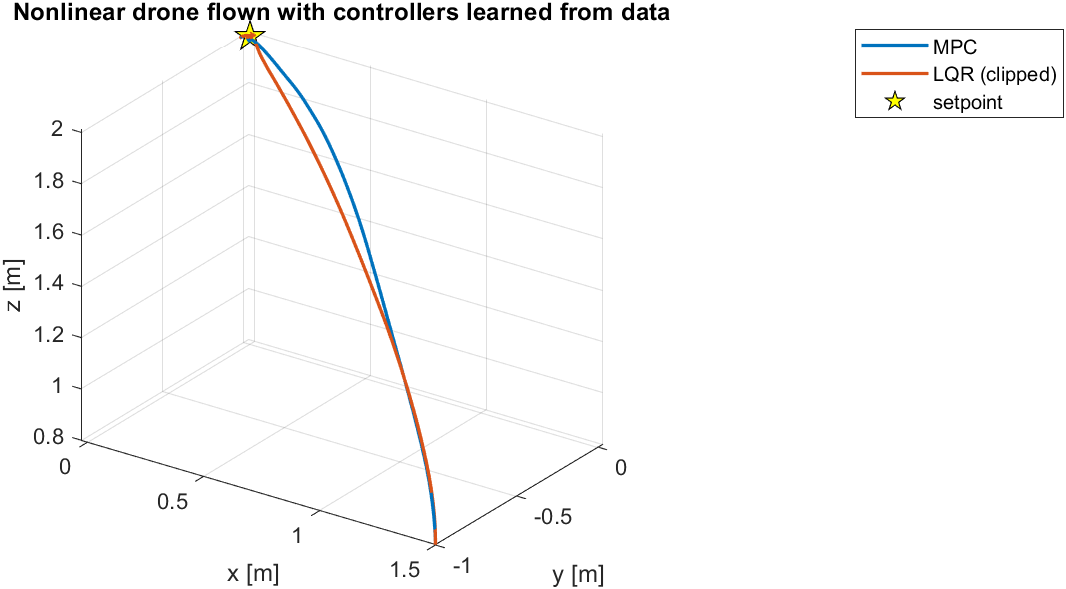
\includegraphics[width=0.6\linewidth]{M2_3_MPC_QP_Apply_to_Drone_2.png}
  \caption{The nonlinear drone flown by MPC and by LQR, both designed only from recorded data.}
\end{figure}

\begin{real}[Model 2]
Model~2 is not inside our ROS~2 node today; it is the data-driven alternative we studied and tested in the toy model. It
plugs into the same place as the SO(3) controller: it takes the state from \code{/ap/v1/pose/filtered} and
\code{/ap/v1/twist/filtered} (converted to $\vx_k$ with (M2.1)) and produces a command. Because ArduPilot accepts velocities,
the practical first step would be an MPC whose output is the velocity $\vv_{\text{cmd}}$ with the limit $\|\vv\|\le1$\,m/s written
into the problem, instead of the clip in \code{publish\_velocity\_command()}.
\end{real}

\subsection*{Recap of Model 2}
\begin{center}\small
\begin{tabularx}{\linewidth}{@{}c >{\raggedright\arraybackslash}p{2.6cm} >{\raggedright\arraybackslash}p{2.7cm} >{\raggedright\arraybackslash}p{2.5cm} X@{}}
\toprule
\textbf{\#} & \textbf{Block} & \textbf{In} & \textbf{Out} & \textbf{The idea in one sentence}\\
\midrule
1 & Flight data & drone, random pushes & $\{\vx_k\},\{\vu_k\}$ & Record what the drone did and what we told it, as differences from hover.\\
2 & DMDc & $X$, $X^+$, $U$ & $A$, $B$ & Least squares finds the linear rule that best predicts the next sample.\\
3 & Bellman & $A,B,Q,R$ & $V=\vx^\top P\vx$ & Best plan = best first move + best plan from where it leads.\\
4 & LQR & $A,B,R,P$ & $K$ & The bottom of a quadratic bowl is a linear law $\vu=-K\vx$.\\
5 & Riccati & $P_0$ & $P_\infty$ & Look one more step ahead each time until nothing changes.\\
6 & DARE & $A,B,Q,R$ & $P$, $K$ & Jump straight to that limit; $\vx_0^\top P\vx_0$ is the total score.\\
7 & MPC & model, limits, $P_f$ & a problem & Plan the next second without breaking any rule.\\
8 & QP & problem, $\vx_0$ & $H,\bm f,G,\bm h$, $\mathbf U^*$ & A bowl inside a fence; one bottom, found in milliseconds.\\
9 & Receding horizon & $\vx_k$ & $\vu_0^*$ & Use the first move only, then plan again.\\
10 & Apply to drone & $\vu_0^*$ or $-K\vx_k$ & $\Omega_1..\Omega_4$ & Add hover thrust back, share among the rotors, fly.\\
\bottomrule
\end{tabularx}
\end{center}

% =====================================================================
\section{How Everything Fits Together}
\label{sec:together}
% =====================================================================

\subsection{One trip around the loop, in words}

Follow the drone for one 40\,ms step of \cref{fig:loop}, with every equation in its place.

\begin{enumerate}
  \item \textbf{The drone moves} according to Newton and Euler, equations (1)--(4). Wind pushes it a little.
  \item \textbf{The sensors measure it.} The gyroscope reads $\vw$ 100 times a second. The camera takes a picture 25 times a
        second; visual odometry compares it with the previous pictures and gives a pose $(\tilde\vp,\tilde R)$. These same poses,
        together with the images, are what the 3D map is built from.
  \item \textbf{The estimator (VIO) works out the state.} Between camera frames it predicts with the physics, equations
        (10)--(11), using the Jacobians of blocks 2--3. When a measurement arrives, it corrects, equations (12)--(14), trusting
        each source according to its noise. Result: $\hx=(\hp,\hv,\hR,\hw)$, published on \code{/ap/v1/*/filtered}.
  \item \textbf{Our node checks the estimate} is fresh and finite (\code{state\_is\_valid}).
  \item \textbf{Where should I be?} The waypoint generator gives $\vp_d=[0,0,2]$, $\psi_d=0$.
  \item \textbf{How should I accelerate?} Position errors and the spring-damper law, equations (15)--(16).
  \item \textbf{Which way should I lean, and how hard should I push?} Equations (17)--(19) give $\vF_d$ and $R_d$.
  \item \textbf{How should I twist?} The SO(3) attitude law, equations (20)--(22), gives $\vtau$; equation (23) gives $T$.
  \item \textbf{What do we send?} Our node publishes all of these for monitoring and sends the velocity
        $\vv_{\text{cmd}}=0.8\ve_p+0.2\ve_v$ (at most 1\,m/s) to ArduPilot.
  \item \textbf{ArduPilot finishes the job}: its own velocity, attitude and rate loops produce $T$ and $\vtau$, and its mixer,
        equations (24)--(25), sets the four motor speeds. The drone moves, and we are back at step 1.
\end{enumerate}

\subsection{Model 1 or Model 2?}

\begin{center}\small
\begin{tabularx}{\linewidth}{@{}l X X@{}}
\toprule
 & \textbf{Model 1 (physics)} & \textbf{Model 2 (data)}\\
\midrule
Where the model comes from & Newton and Euler; needs $m$, $J$, rotor data & Recorded flights (DMDc); needs nothing measured by hand\\
Kind of model & Nonlinear, attitude as a rotation matrix & Linear, near hover, attitude as 3 small angles\\
Works for & Any attitude except upside down & Small tilts (in our data, below 6.5$^\circ$)\\
Controller & Geometric: position loop $\rightarrow$ attitude loop & LQR (a fixed gain table) or MPC (a small optimisation every step)\\
Limits (speed, thrust, tilt) & Only by clipping afterwards & Written into the MPC problem itself\\
Cost per step on the drone & A few $3\times3$ matrix products & LQR: one $4\times12$ product; MPC: a QP of about 2.6\,ms\\
Where in our project & \code{so3\_controller.py}, \code{controller\_node.py} & Toy model \code{M2\_1}--\code{M2\_3}\\
\bottomrule
\end{tabularx}
\end{center}

The two are not rivals. Model~1's estimator provides the state that Model~2's controllers need, and Model~2's DMDc is a
check on Model~1's physics: the learned $A$ and $B$ agree with the Jacobians of block 2 to about 1--3\%, and the data
reproduces the 1.5\,kg mass to within 0.4\%.

\subsection{Why the camera matters for control}

The single most important link in the whole chain is the estimate $\hx$. Every controller in this document (SO(3), LQR,
MPC, and ArduPilot's own) works only as well as the state it is given. Block 3 showed why an IMU alone fails: a tiny
gyro error grows into metres of position error within seconds ($t^3$). The monocular camera, through VIO, is what keeps
that error at a few centimetres (block 4: 2.6\,cm instead of drifting away). That is the meaning of the title of our
project: the drone is \emph{controlled by} visual-inertial odometry, and the same camera poses build the 3D map.

\clearpage
% =====================================================================
\section{Using the Toy Model}
\label{sec:toyguide}
% =====================================================================

\subsection{The files}

\begin{center}\small
\begin{tabularx}{\linewidth}{@{}l l X@{}}
\toprule
\textbf{File in \code{toy\_model3/}} & \textbf{Blocks} & \textbf{What you see when you run it}\\
\midrule
\code{M1\_1\_Dynamics\_Linearization.mlx} & M1: 1--3 & hover check, 10$^\circ$ tilt, gyroscopic coupling, open-loop drift (\code{ode45}), Jacobians and their numerical check, linear vs.\ nonlinear error\\
\code{M1\_2\_Error\_State\_EKF.mlx} & M1: 4 & the altitude filter by hand, then the full 12-state filter with camera and gyro, accuracy and the $3\sigma$ band\\
\code{M1\_3\_SO3\_Control\_Closed\_Loop.mlx} & M1: 5--8 & each control equation with the toy numbers, recovery from 60$^\circ$, the motor mixer, the full closed loop, the velocity command of our node\\
\code{M2\_1\_Flight\_Data\_DMDc.mlx} & M2: 1--2 & recording five flights, DMDc by hand and on the drone, comparison with physics, test on unseen data\\
\code{M2\_2\_LQR\_Bellman\_Riccati\_DARE.mlx} & M2: 3--6 & Bellman step, Riccati table, scalar DARE, the drone's $K$, cost check\\
\code{M2\_3\_MPC\_QP\_Apply\_to\_Drone.mlx} & M2: 7--10 & two-step QP by hand, the drone MPC, MPC = LQR when no limit is active, receding horizon, nonlinear flight\\
\code{DroneLib.m} & all & the helper functions: dynamics, RK4, Exp/Log, Jacobians, controller, mixer, EKF steps, DARE, QP solver\\
\code{pdf/*.mlx.pdf} & all & every live script already run and exported, with all outputs and figures\\
\bottomrule
\end{tabularx}
\end{center}

\subsection{How to run them}

\begin{enumerate}
  \item Open MATLAB (tested with R2024a; no toolboxes are needed) and make \code{toy\_model3} the current folder, because
        every script calls \code{DroneLib}.
  \item Open a live script and press \emph{Run}, or run it section by section (\emph{Run Section}) while reading this document.
  \item Model~2 files must be run in order: \code{M2\_1} creates \code{dmdc\_model.mat} (the learned $A$, $B$),
        \code{M2\_2} adds the LQR results to it, and \code{M2\_3} uses both.
  \item To export a live script as PDF, change \code{PUBLISH = not(ready);} at the top to \code{PUBLISH = ready;}. The last
        section then writes \code{pdf/<name>.mlx.pdf}, exactly like the course notes.
\end{enumerate}

\subsection{How each live script is organised}

Every file follows the same pattern as the course notes: a header, then for each block an orange title, the equations in
LaTeX with their numbers $(1),(2),\dots$ or $(M2.x)$, a short derivation, a toy example with hand-checkable numbers, and the
code that reproduces those numbers. Sections that start a new topic begin with \code{clearvars -except PUBLISH ready}, so
each part can be run on its own.

\subsection{Things to try}

\begin{itemize}
  \item In the closed-loop section of \code{M1\_3}, add \code{P.Kv = 2*P.Kv;} after \code{P = DroneLib.params();} (a stronger
        damper) or \code{P.Kp = 0.5*P.Kp;} (a weaker spring), run it again and compare \code{tracking\_rmse\_cm}.
  \item In \code{M1\_2}, make the camera noise ten times larger (\code{sig\_p = 0.5}) and see $K$ trust the camera less.
  \item In \code{M2\_1}, remove the random pushes (\code{exc = zeros(4,1)}) and watch \code{rank\_Omega} drop below 16: DMDc can
        no longer tell the drone from the pilot.
  \item In \code{M2\_3}, change the speed limit \code{x\_max(1:3)} to 0.5\,m/s and see MPC fly more slowly but still reach the target.
\end{itemize}

\appendix
% =====================================================================
\section{All Symbols in One Table}
\label{app:symbols}
% =====================================================================

\begin{center}\small
\begin{tabularx}{\linewidth}{@{}l X l l@{}}
\toprule
\textbf{Symbol} & \textbf{Meaning} & \textbf{Size} & \textbf{Unit}\\
\midrule
$\vp,\ \vv$ & position, velocity (world, ENU) & 3 & m, m/s\\
$R$ & attitude: body $\rightarrow$ world rotation matrix & $3\times3$ & --\\
$\vw$ & angular velocity in the body frame & 3 & rad/s\\
$T,\ \vtau$ & total thrust, body torque & 1, 3 & N, N\,m\\
$\vu=[T;\vtau]$ & input & 4 & N, N\,m\\
$m,\ J,\ g_0$ & mass, inertia, gravity & 1, $3\times3$, 1 & kg, kg\,m$^2$, m/s$^2$\\
$\ve_3$ & $[0,0,1]^\top$ & 3 & --\\
$\skw{\bm a}$, $(\cdot)^\vee$ & hat (cross-product matrix), vee (its inverse) & $3\times3$, 3 & --\\
$\Exp,\ \Log$ & rotation vector $\leftrightarrow$ rotation matrix & -- & rad\\
$\hat{(\cdot)},\ (\cdot)_d,\ \tilde{(\cdot)}$ & estimated, desired, measured & -- & --\\
$\delta\vx$ & error state $[\delta\vp;\delta\vv;\delta\vth;\delta\vw]$ & 12 & m, m/s, rad, rad/s\\
$A,\ B$ & Jacobians (Model 1) or learned model (Model 2) & $12\times12$, $12\times4$ & --\\
$F$ & one-step error transition & $12\times12$ & --\\
$P$ (EKF) & error covariance & $12\times12$ & squared units\\
$Q,\ R_n$ (EKF) & process noise, sensor noise covariance & $12\times12$, $m\times m$ & squared units\\
$H,\ K$ (EKF) & measurement Jacobian, Kalman gain & $m\times12$, $12\times m$ & --\\
$\ve_p,\ \ve_v$ & position, velocity error & 3 & m, m/s\\
$K_p,\ K_v$ & position, velocity gains & $3\times3$ & 1/s$^2$, 1/s\\
$\va_d,\ \vF_d$ & desired acceleration, desired force & 3 & m/s$^2$, N\\
$\vb_{1d},\vb_{2d},\vb_{3d},\ R_d$ & desired body axes, desired attitude & 3, $3\times3$ & --\\
$\psi_d$ & desired yaw & 1 & rad\\
$\ve_R,\ \ve_\omega$ & attitude error, angular-velocity error & 3 & rad, rad/s\\
$K_R,\ K_\omega$ & attitude, rate gains & $3\times3$ & N\,m, N\,m\,s\\
$\Gamma,\ \vf,\ \vOmega$ & mixer matrix, rotor thrusts, motor speeds & $4\times4$, 4, 4 & --, N, rad/s\\
$k_f,\ c_m$ & thrust constant, yaw torque per newton & 1 & N\,s$^2$, m\\
$X,\ X^+,\ U$ & snapshot matrices (DMDc) & $12\times N$, $4\times N$ & --\\
$Q,\ R$ (control) & state weight, input weight & $12\times12$, $4\times4$ & --\\
$P$ (control) & value matrix: $V(\vx)=\vx^\top P\vx$ & $12\times12$ & --\\
$K$ (control) & LQR gain, $\vu=-K\vx$ & $4\times12$ & --\\
$N,\ P_f$ & MPC horizon, terminal weight & 1, $12\times12$ & steps, --\\
$S_x,\ S_u,\ H,\ \bm f,\ G,\ \bm h$ & QP matrices & see block 8 & --\\
$\vv_{\text{cmd}}$ & velocity command sent by our node & 3 & m/s\\
\bottomrule
\end{tabularx}
\end{center}

% =====================================================================
\section{Glossary}
% =====================================================================

\begin{center}\small
\begin{tabularx}{\linewidth}{@{}l X@{}}
\toprule
\textbf{Word} & \textbf{Meaning in plain words}\\
\midrule
ArduPilot SITL & the real flight-controller software, running on a PC and flying a simulated drone\\
Attitude & which way the drone is facing and tilted; stored as the matrix $R$\\
Covariance & a table of ``how unsure'' for every error and every pair of errors\\
DARE & the equation whose solution gives the best LQR gain for an endless flight\\
DMDc & learning $\vx_{k+1}=A\vx_k+B\vu_k$ from recorded data by least squares\\
EKF & Extended Kalman Filter: predict with the model, correct with sensors, weighted by trust\\
ENU / FLU & world axes East-North-Up / body axes Forward-Left-Up\\
Error state & the filter keeps track of the small error, not the full state, so the attitude stays a true rotation\\
Gimbal lock & the failure of roll-pitch-yaw angles at 90$^\circ$ pitch; avoided by using $R$\\
IMU & Inertial Measurement Unit: gyroscope and accelerometer\\
Innovation & what the sensor says minus what we expected it to say\\
Jacobian & the matrix of all ``slopes'' of a function of many variables\\
Kalman gain & how far to move the estimate towards a measurement\\
Linearization & replacing a curved model by its tangent (straight-line) version near a point\\
LQR & the best linear controller for a quadratic score: $\vu=-K\vx$\\
Lyapunov function & an ``energy'' that can only decrease; proves that a controller settles\\
MPC & re-plan the next few seconds at every step, with limits, and use only the first move\\
QP & quadratic program: find the bottom of a bowl inside a fence\\
ROS~2 & software that lets programs exchange messages on named topics\\
SO(3) & the set of all rotation matrices\\
VIO & Visual-Inertial Odometry: working out motion from a camera and an IMU together\\
\bottomrule
\end{tabularx}
\end{center}

% =====================================================================
\section{References}
% =====================================================================

\begin{enumerate}[label={[\arabic*]}, leftmargin=*]
\item T.~Lee, M.~Leok, N.\,H.~McClamroch, ``Geometric tracking control of a quadrotor UAV on SE(3)'', IEEE CDC, 2010.
      (Blocks 5--7 of Model 1.)
\item J.~Sol\`a, ``Quaternion kinematics for the error-state Kalman filter'', arXiv:1711.02508, 2017. (Block 4.)
\item J.\,L.~Proctor, S.\,L.~Brunton, J.\,N.~Kutz, ``Dynamic mode decomposition with control'', SIAM J.\ Applied Dynamical
      Systems 15(1), 2016. (Model 2, block 2.)
\item D.\,P.~Bertsekas, \emph{Dynamic Programming and Optimal Control}, Vol.~I. (Model 2, blocks 3--6.)
\item J.\,B.~Rawlings, D.\,Q.~Mayne, M.\,M.~Diehl, \emph{Model Predictive Control: Theory, Computation, and Design}, 2nd ed., 2017.
      (Model 2, blocks 7--9.)
\item T.~Qin, P.~Li, S.~Shen, ``VINS-Mono: a robust and versatile monocular visual-inertial state estimator'', IEEE T-RO, 2018.
\item Sunil Kumar~S and K.\,P.~Soman, course notes \emph{Introduction to Drones -- 22AIE448}: ``Taylor series'' and
      ``Nonlinear systems and EDMD'', Amrita Vishwa Vidyapeetham.
\item ArduPilot documentation: SITL with Gazebo, ROS~2 (DDS) interface. Project parameters: \code{drones\_controller/config/controller.yaml}.
\end{enumerate}


\end{document}
